% !TeX spellcheck = en_US
% !TeX encoding = utf8
% !TeX program = xelatex
% !BIB program = bibtex
% \documentclass[mathserif,compress,12pt]{ctexbeamer}
\documentclass[12pt,notes,mathserif]{beamer}
% \documentclass[draft]{beamer}	
\usetheme{Singapore}
% \usetheme{Hannover}
%\usepackage{pgfpages}
%\setbeameroption{show notes on second screen}

\usepackage[british]{babel}
\usepackage{graphicx,hyperref,url}
% \usepackage{ru}
\usepackage{mmstyles,bm,ulem}

\usepackage{listings}
\usefonttheme[onlymath]{serif}
\usepackage{fontspec}
\usepackage{xeCJK}
% \pgfdeclareimage[width=\paperwidth,height=\paperheight]{bg}{background}
% \setbeamertemplate{background}{\pgfuseimage{bg}}
%% columns
\newcommand{\begincols}[1]{\begin{columns}{#1}}
\newcommand{\stopcols}{\end{columns}}
% \usepackage[backend=biber]{biblatex}
% \bibliography{./ref.bib}
%\addbibresource{ref.bib}
\usepackage{indentfirst}
\usepackage{longtable}
\usepackage{float}
%\usepackage{picins}
\usepackage{rotating}
\usepackage{subfigure}
\usepackage{tabu}
\usepackage{amsmath}
\usepackage{amssymb}
\usepackage{setspace}
\usepackage{amsfonts}
\usepackage{appendix}
\usepackage{listings}
\usepackage{xcolor}
\usepackage{colortbl}
\usepackage{geometry}
% \setCJKfamilyfont{cjkhwxk}{SimSun}
% \newcommand*{\cjkhwxk}{\CJKfamily{cjkhwxk}}
%\newfontfamily{\consolas}{Consolas}
%\newfontfamily{\monaco}{Monaco}
%\setmonofont[Mapping={}]{Consolas}	%英文引号之类的正常显示,相当于设置英文字体
%\setsansfont{Consolas} %设置英文字体 Monaco, Consolas,  Fantasque Sans Mono
% \setmainfont{Times New Roman}
% \newfontfamily{\consolas}{Times New Roman}
% \newfontfamily{\monaco}{Arial}
% \setCJKmainfont{Times New Roman}
%\setmainfont{MONACO.TTF}
%\setsansfont{MONACO.TTF}
\newcommand{\verylarge}{\fontsize{60pt}{\baselineskip}\selectfont}  
\newcommand{\chuhao}{\fontsize{44.9pt}{\baselineskip}\selectfont}  
\newcommand{\xiaochu}{\fontsize{38.5pt}{\baselineskip}\selectfont}  
\newcommand{\yihao}{\fontsize{27.8pt}{\baselineskip}\selectfont}  
\newcommand{\xiaoyi}{\fontsize{25.7pt}{\baselineskip}\selectfont}  
\newcommand{\erhao}{\fontsize{23.5pt}{\baselineskip}\selectfont}  
\newcommand{\xiaoerhao}{\fontsize{19.3pt}{\baselineskip}\selectfont} 
\newcommand{\sihao}{\fontsize{14pt}{\baselineskip}\selectfont}      % 字号设置  
\newcommand{\xiaosihao}{\fontsize{12pt}{\baselineskip}\selectfont}  % 字号设置  
\newcommand{\wuhao}{\fontsize{10.5pt}{\baselineskip}\selectfont}    % 字号设置  
\newcommand{\xiaowuhao}{\fontsize{9pt}{\baselineskip}\selectfont}   % 字号设置  
\newcommand{\liuhao}{\fontsize{7.875pt}{\baselineskip}\selectfont}  % 字号设置  
\newcommand{\qihao}{\fontsize{5.25pt}{\baselineskip}\selectfont}    % 字号设置 

\graphicspath{{./fig/}}

% \setbeamertemplate{footnote}{%
%   \hangpara{2em}{1}%
%   \makebox[2em][l]{\insertfootnotemark}\footnotesize\insertfootnotetext\par%
% }

\definecolor{cred}{rgb}{0.6,0,0}
\definecolor{cgreen}{rgb}{0.25,0.5,0.35}
\definecolor{cpurple}{rgb}{0.5,0,0.35}
\definecolor{cdocblue}{rgb}{0.25,0.35,0.75}
\definecolor{cdark}{rgb}{0.95,1.0,1.0}
\lstset{
	language=R,
	numbers=left,
	numberstyle=\tiny\color{black},
	keywordstyle=\color{cpurple}\consolas,
	commentstyle=\color{cgreen}\consolas,
	stringstyle=\color{cred}\consolas,
	frame=single,
	escapeinside=``,
	xleftmargin=1em,
	xrightmargin=1em, 
	backgroundcolor=\color{cdark},
	aboveskip=1em,
	breaklines=true,
	tabsize=3
} 

\providecommand{\tightlist}{%
  \setlength{\itemsep}{0pt}\setlength{\parskip}{0pt}}

  
% The title of the presentation:
%  - first a short version which is visible at the bottom of each slide;
%  - second the full title shown on the title slide;
% \title[]{\LARGE CSE 5526: Introduction to Neural Networks}
\title{Support Vector Machines (SVM)}

% Optional: a subtitle to be dispalyed on the title slide
% \subtitle{\Large Support Vector Machines
% (SVM)}

% The author(s) of the presentation:
%  - again first a short version to be displayed at the bottom;
%  - next the full list of authors, which may include contact information;
\author[YingmingLi]{Yingming Li \\ yingming@zju.edu.cn}
% The institute:
%  - to start the name of the university as displayed on the top of each slide
%    this can be adjusted such that you can also create a Dutch version
%  - next the institute information as displayed on the title slide

\institute[DSERC, ZJU]{Data Science \& Engineering Research Center, ZJU}
% Add a date and possibly the name of the event to the slides
%  - again first a short version to be shown at the bottom of each slide
%  - second the full date and event name for the title slide
\date[\today]{\today}
\begin{document}

\AtBeginSection[]
{
	\begin{frame}
		\frametitle{Outline}
		\tableofcontents[currentsection]
	\end{frame}
}

% \AtBeginSubsection[2-]
% {
%    \begin{frame}
%        \frametitle{Outline}
%        \tableofcontents[currentsection]
%    \end{frame}
% }
\begin{frame}[c]
	\titlepage
	% \begin{center}
		% MLP Tips
	% \end{center}
\end{frame}

% 2
\begin{frame}[c]
\frametitle{Perceptrons find any separating hyperplane}
\begin{center}
Depends on initialization and ordering of training points\\
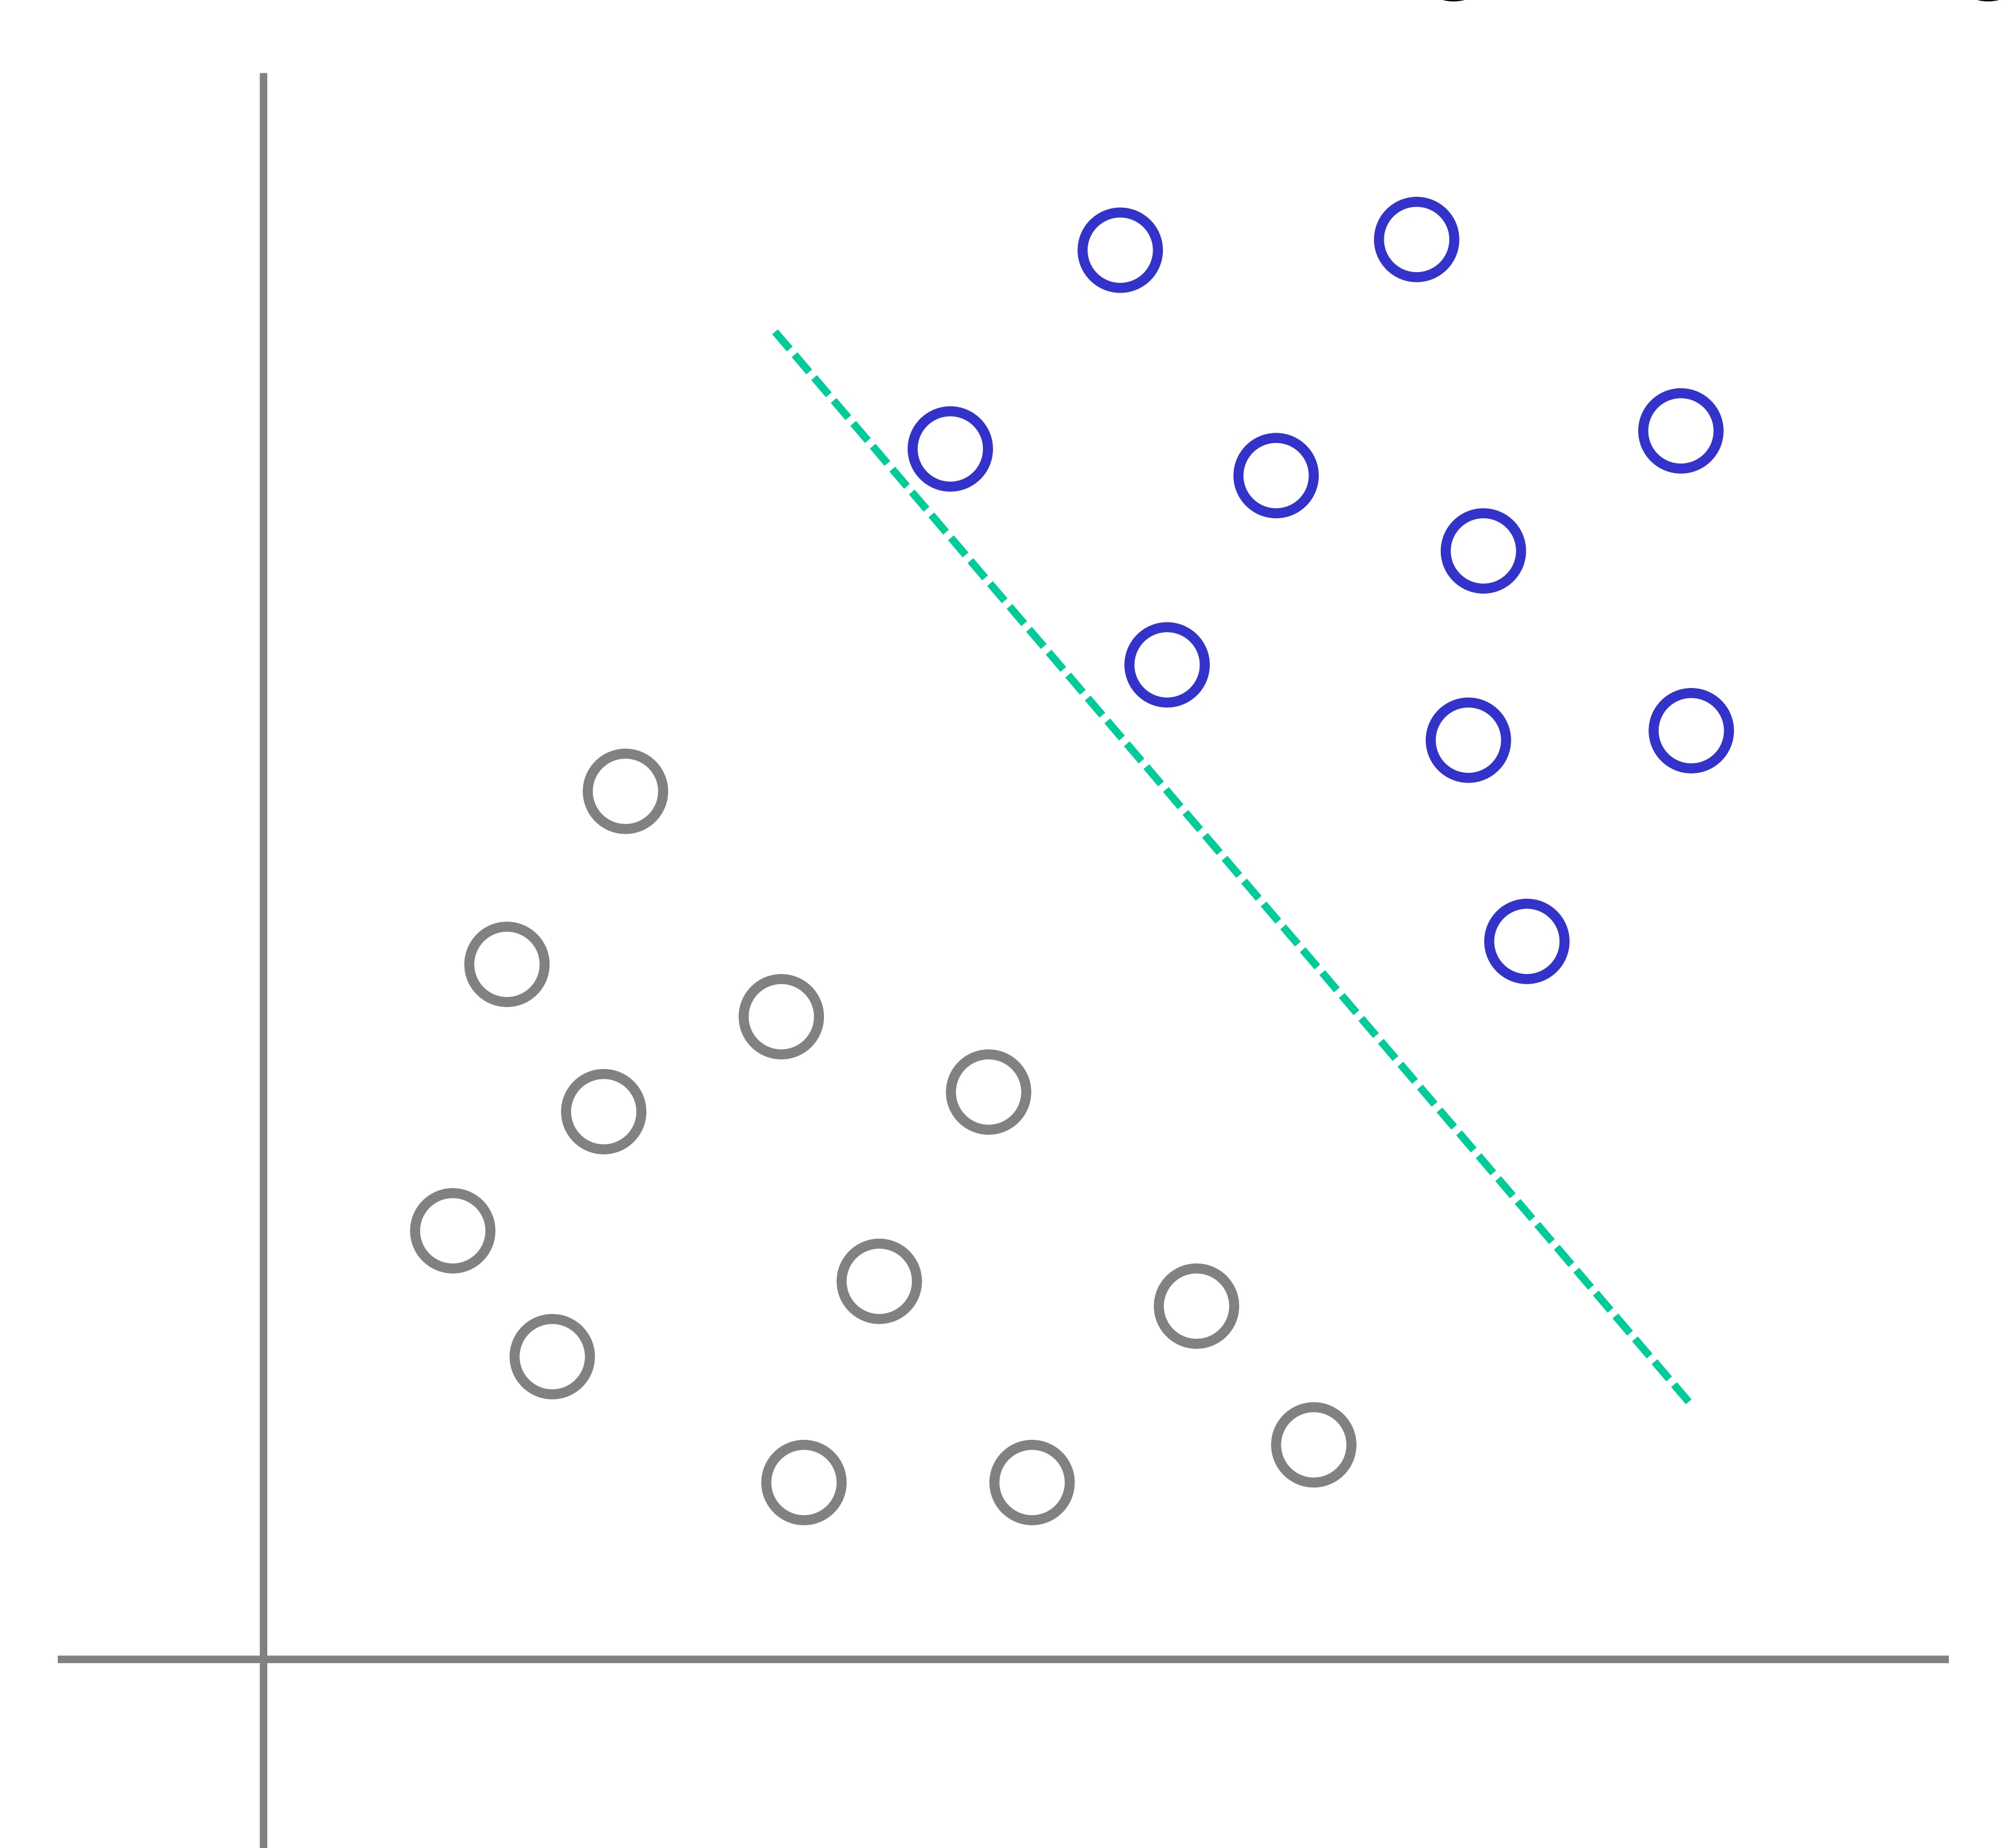
\includegraphics[width=0.7\linewidth]{fig8/lec82.jpg}
\end{center}
\end{frame}
% 3
\begin{frame}[c]
\frametitle{Perceptrons find any separating hyperplane}
\begin{center}
Depends on initialization and ordering of training points\\
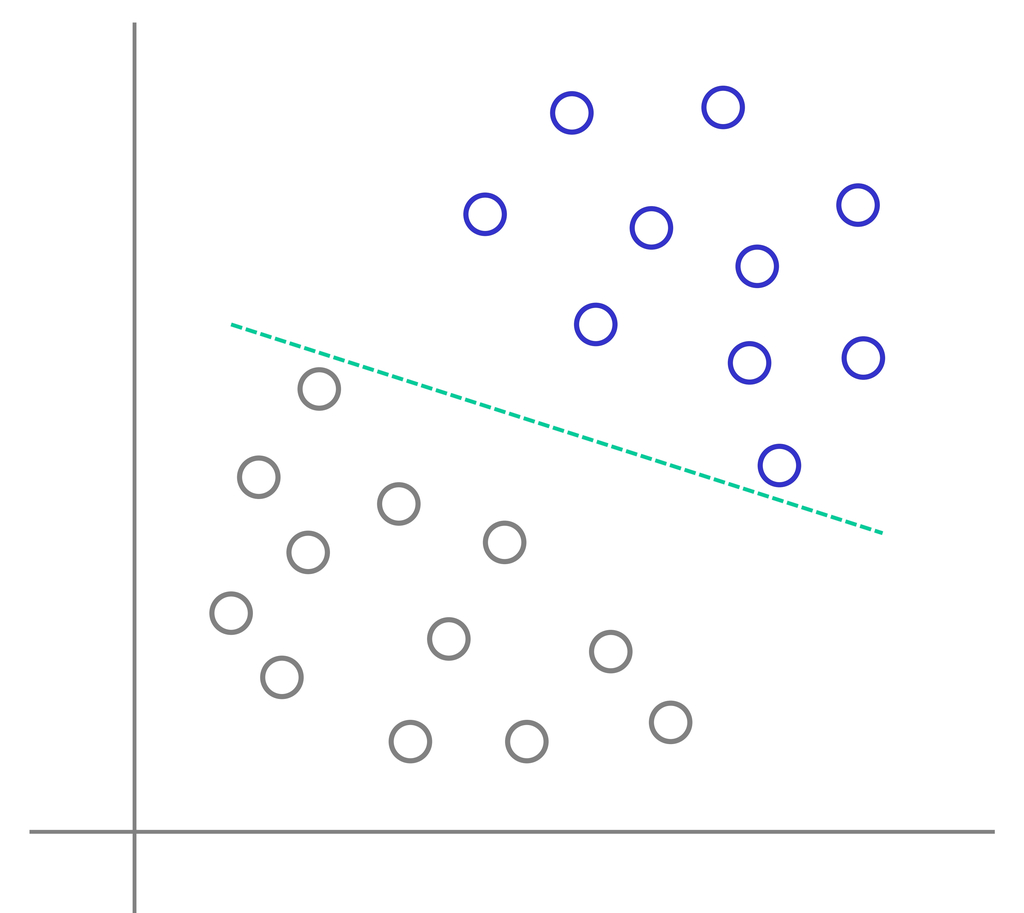
\includegraphics[width=0.7\linewidth]{fig8/lec83.jpg}
\end{center}
\end{frame}

% 4
\begin{frame}[c]
\frametitle{Perceptrons find any separating hyperplane}
\begin{center}
Depends on initialization and ordering of training points\\
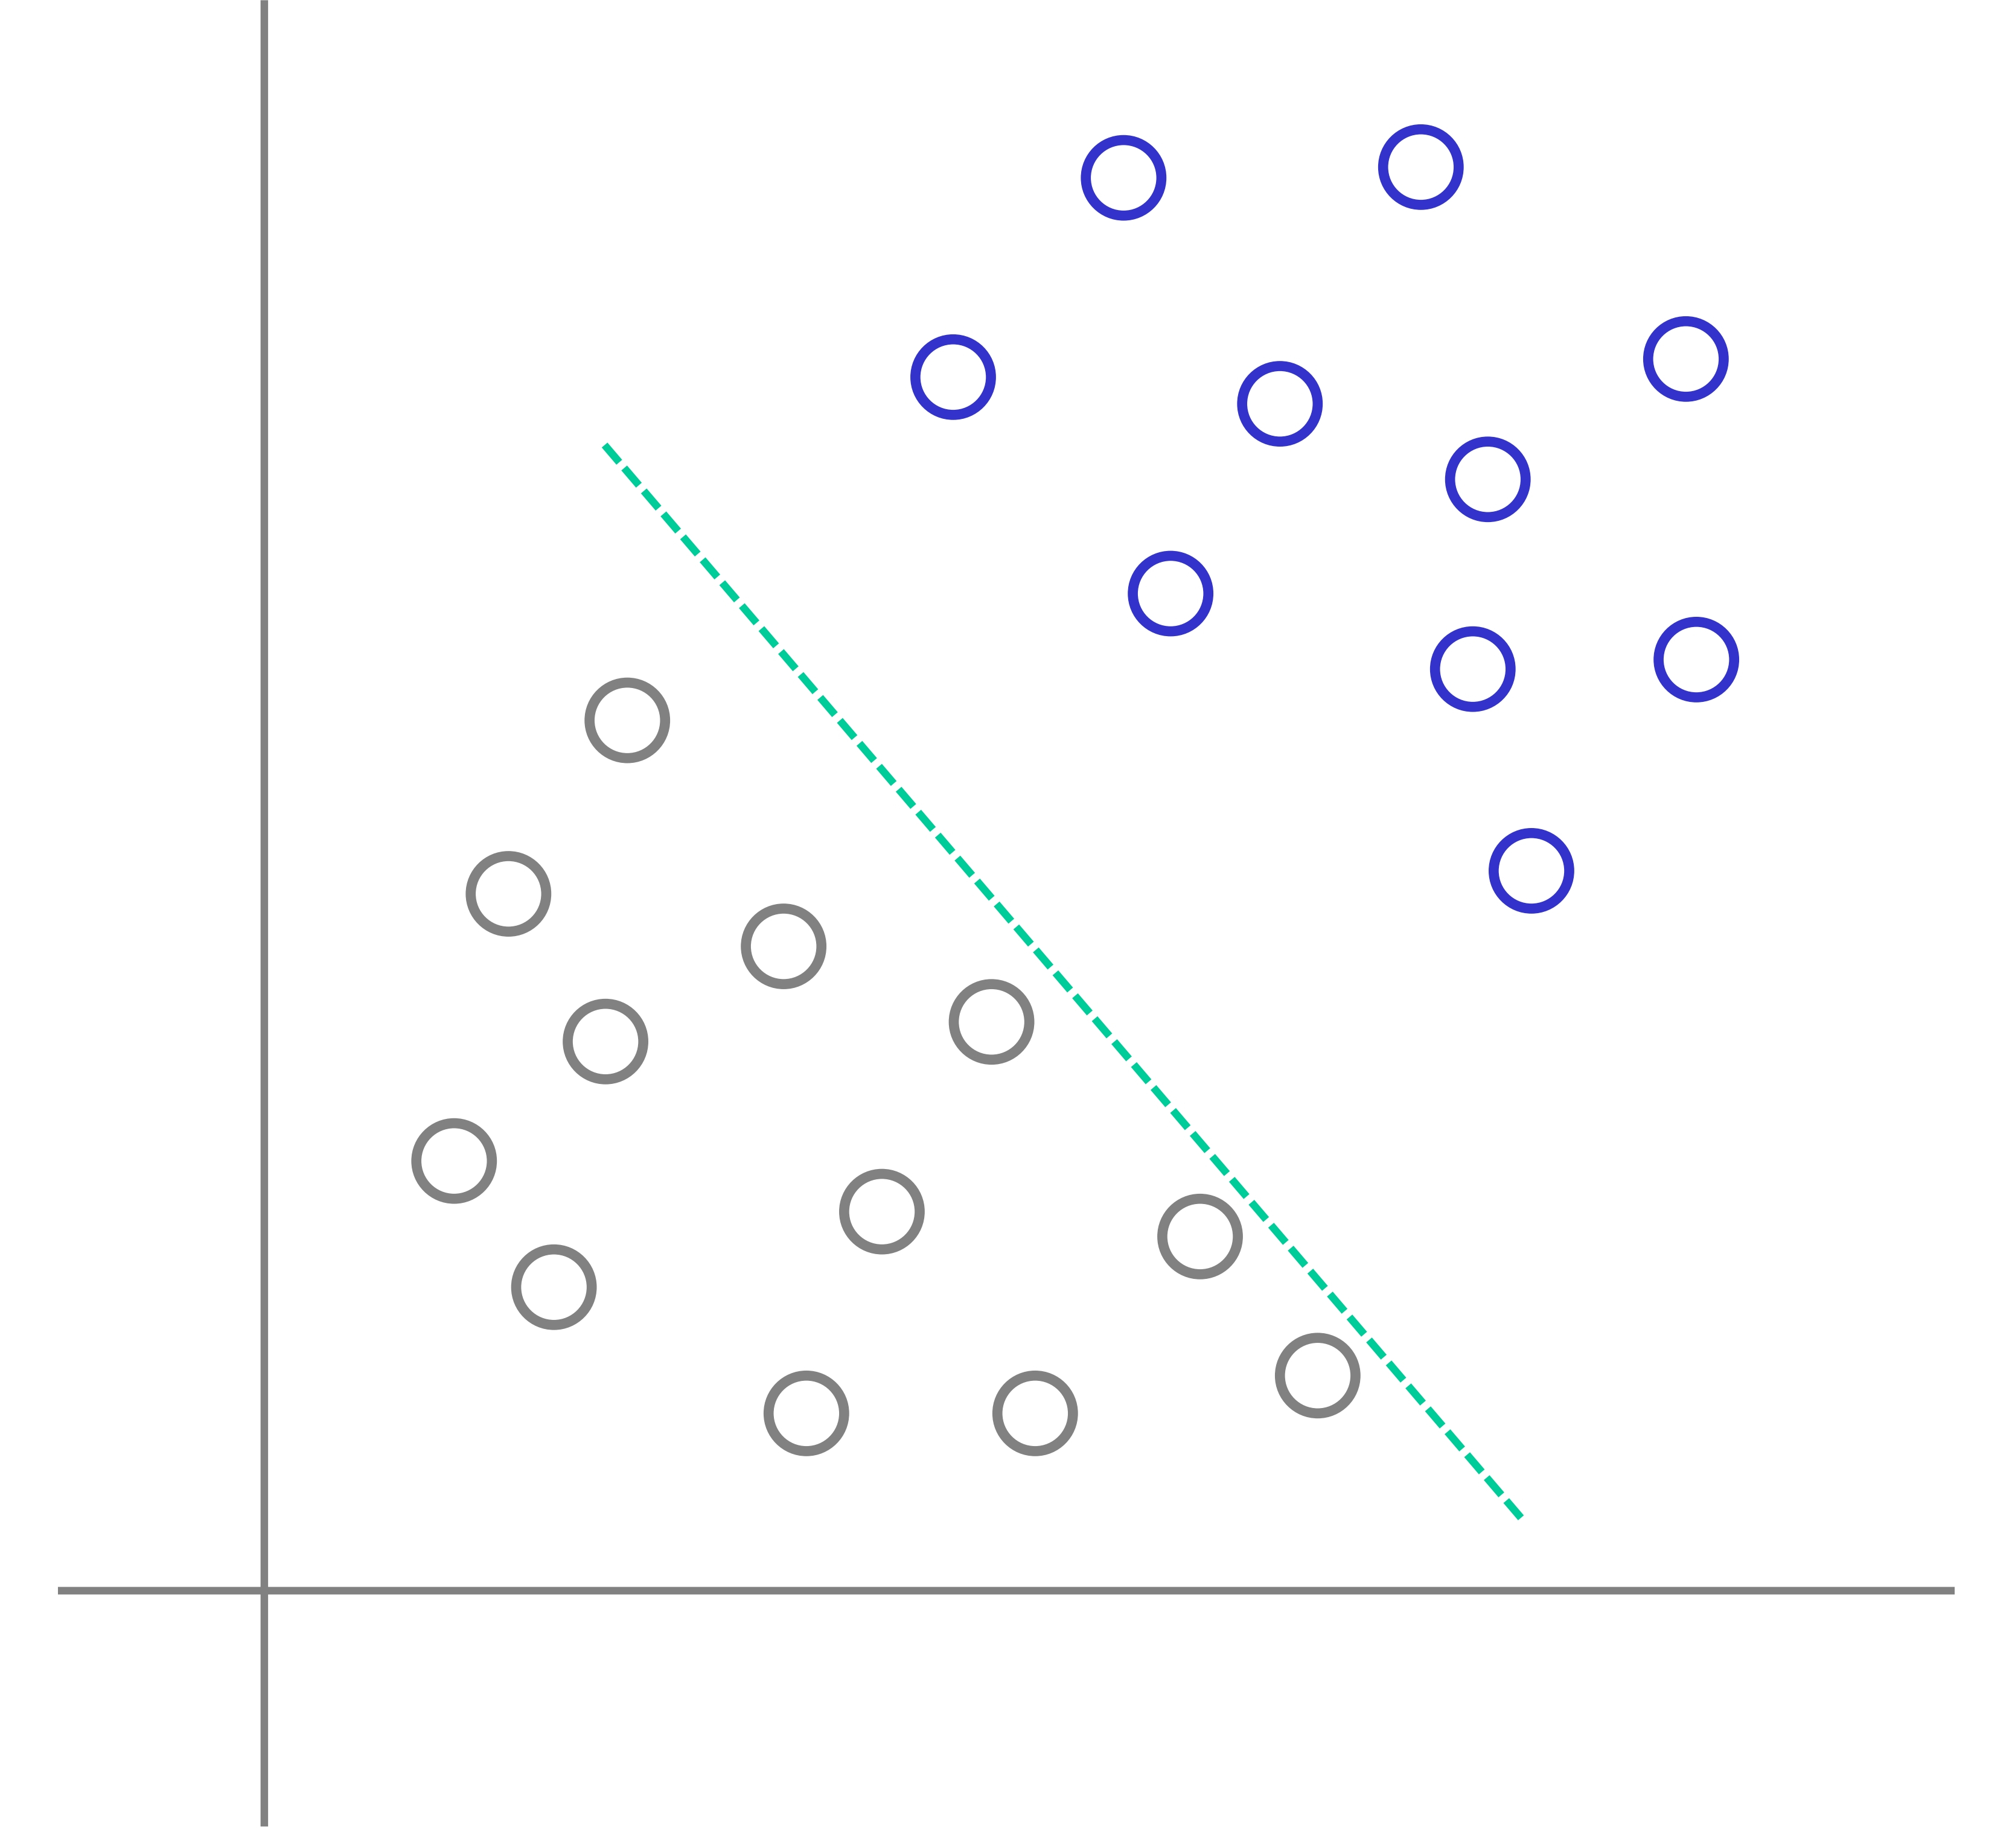
\includegraphics[width=0.7\linewidth]{fig8/lec84.jpg}
\end{center}
\end{frame}

% 5
\begin{frame}[c]
\frametitle{Perceptrons find any separating hyperplane}
\begin{center}
Depends on initialization and ordering of training points\\
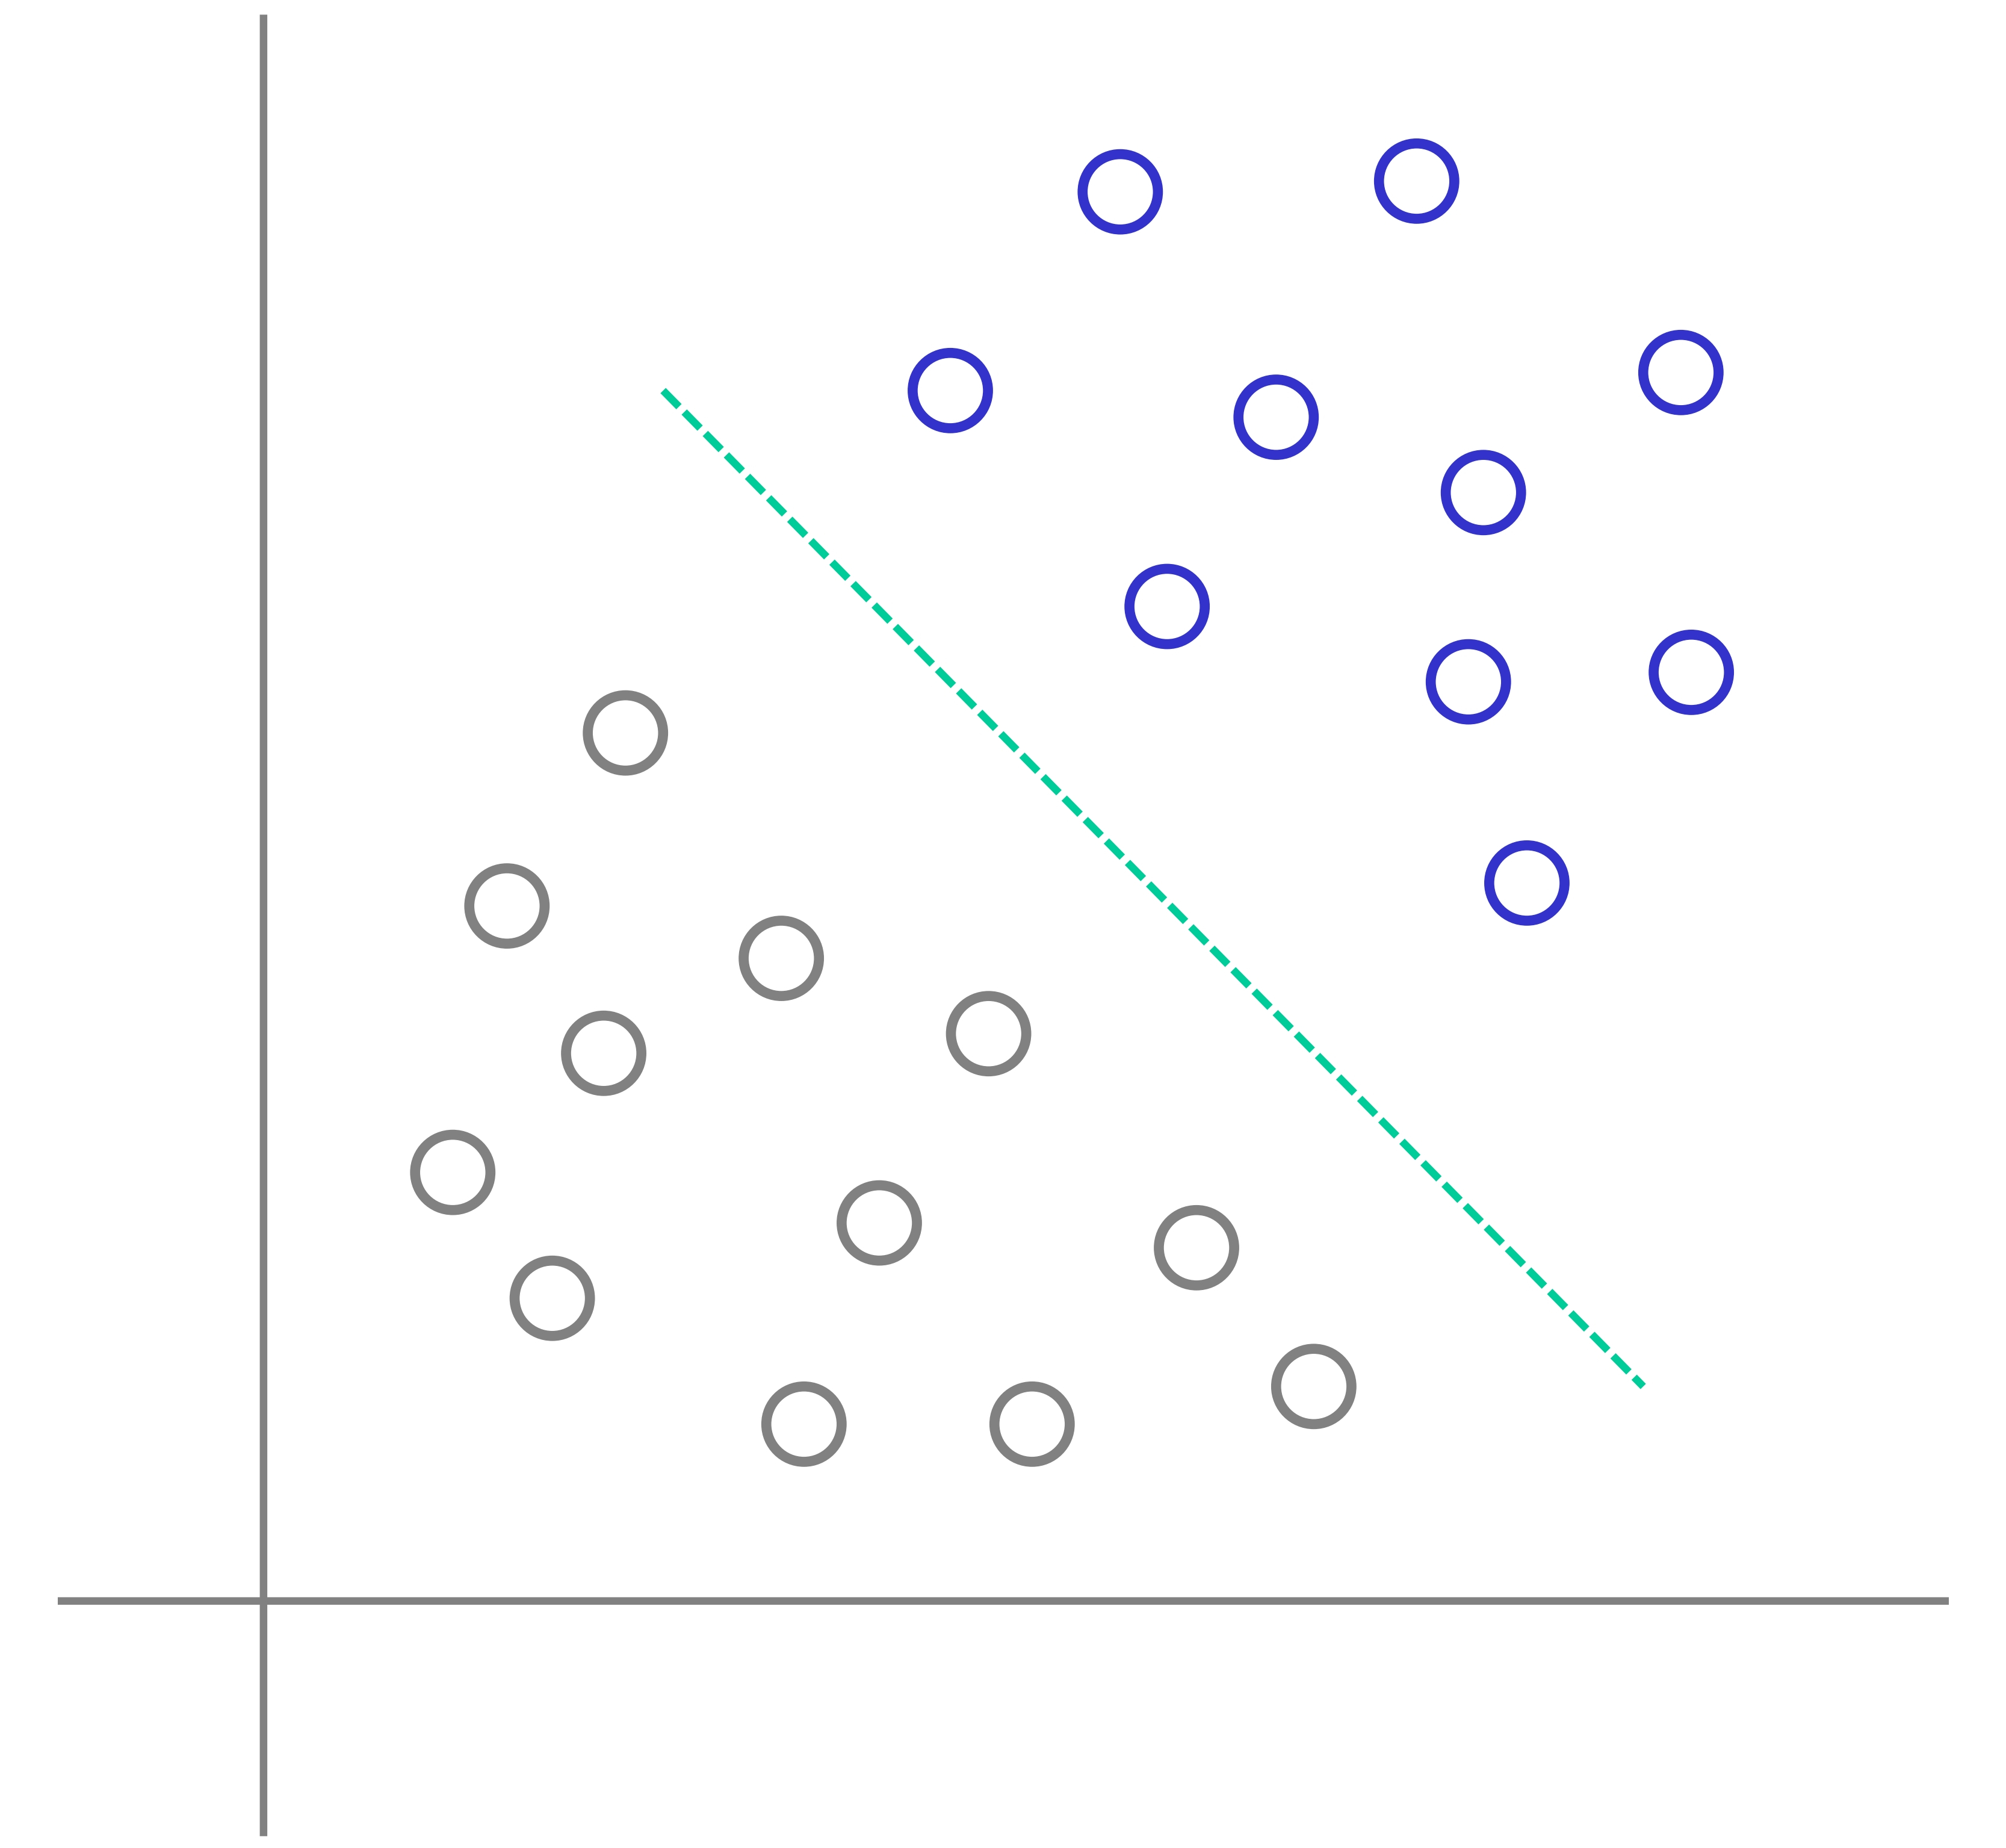
\includegraphics[width=0.7\linewidth]{fig8/lec85.jpg}
\end{center}
\end{frame}



% 6
\begin{frame}[c]
\frametitle{But the maximum margin hyperplane generalizes the best to new data}
\begin{center}
According to computational/statistical learning theory\\
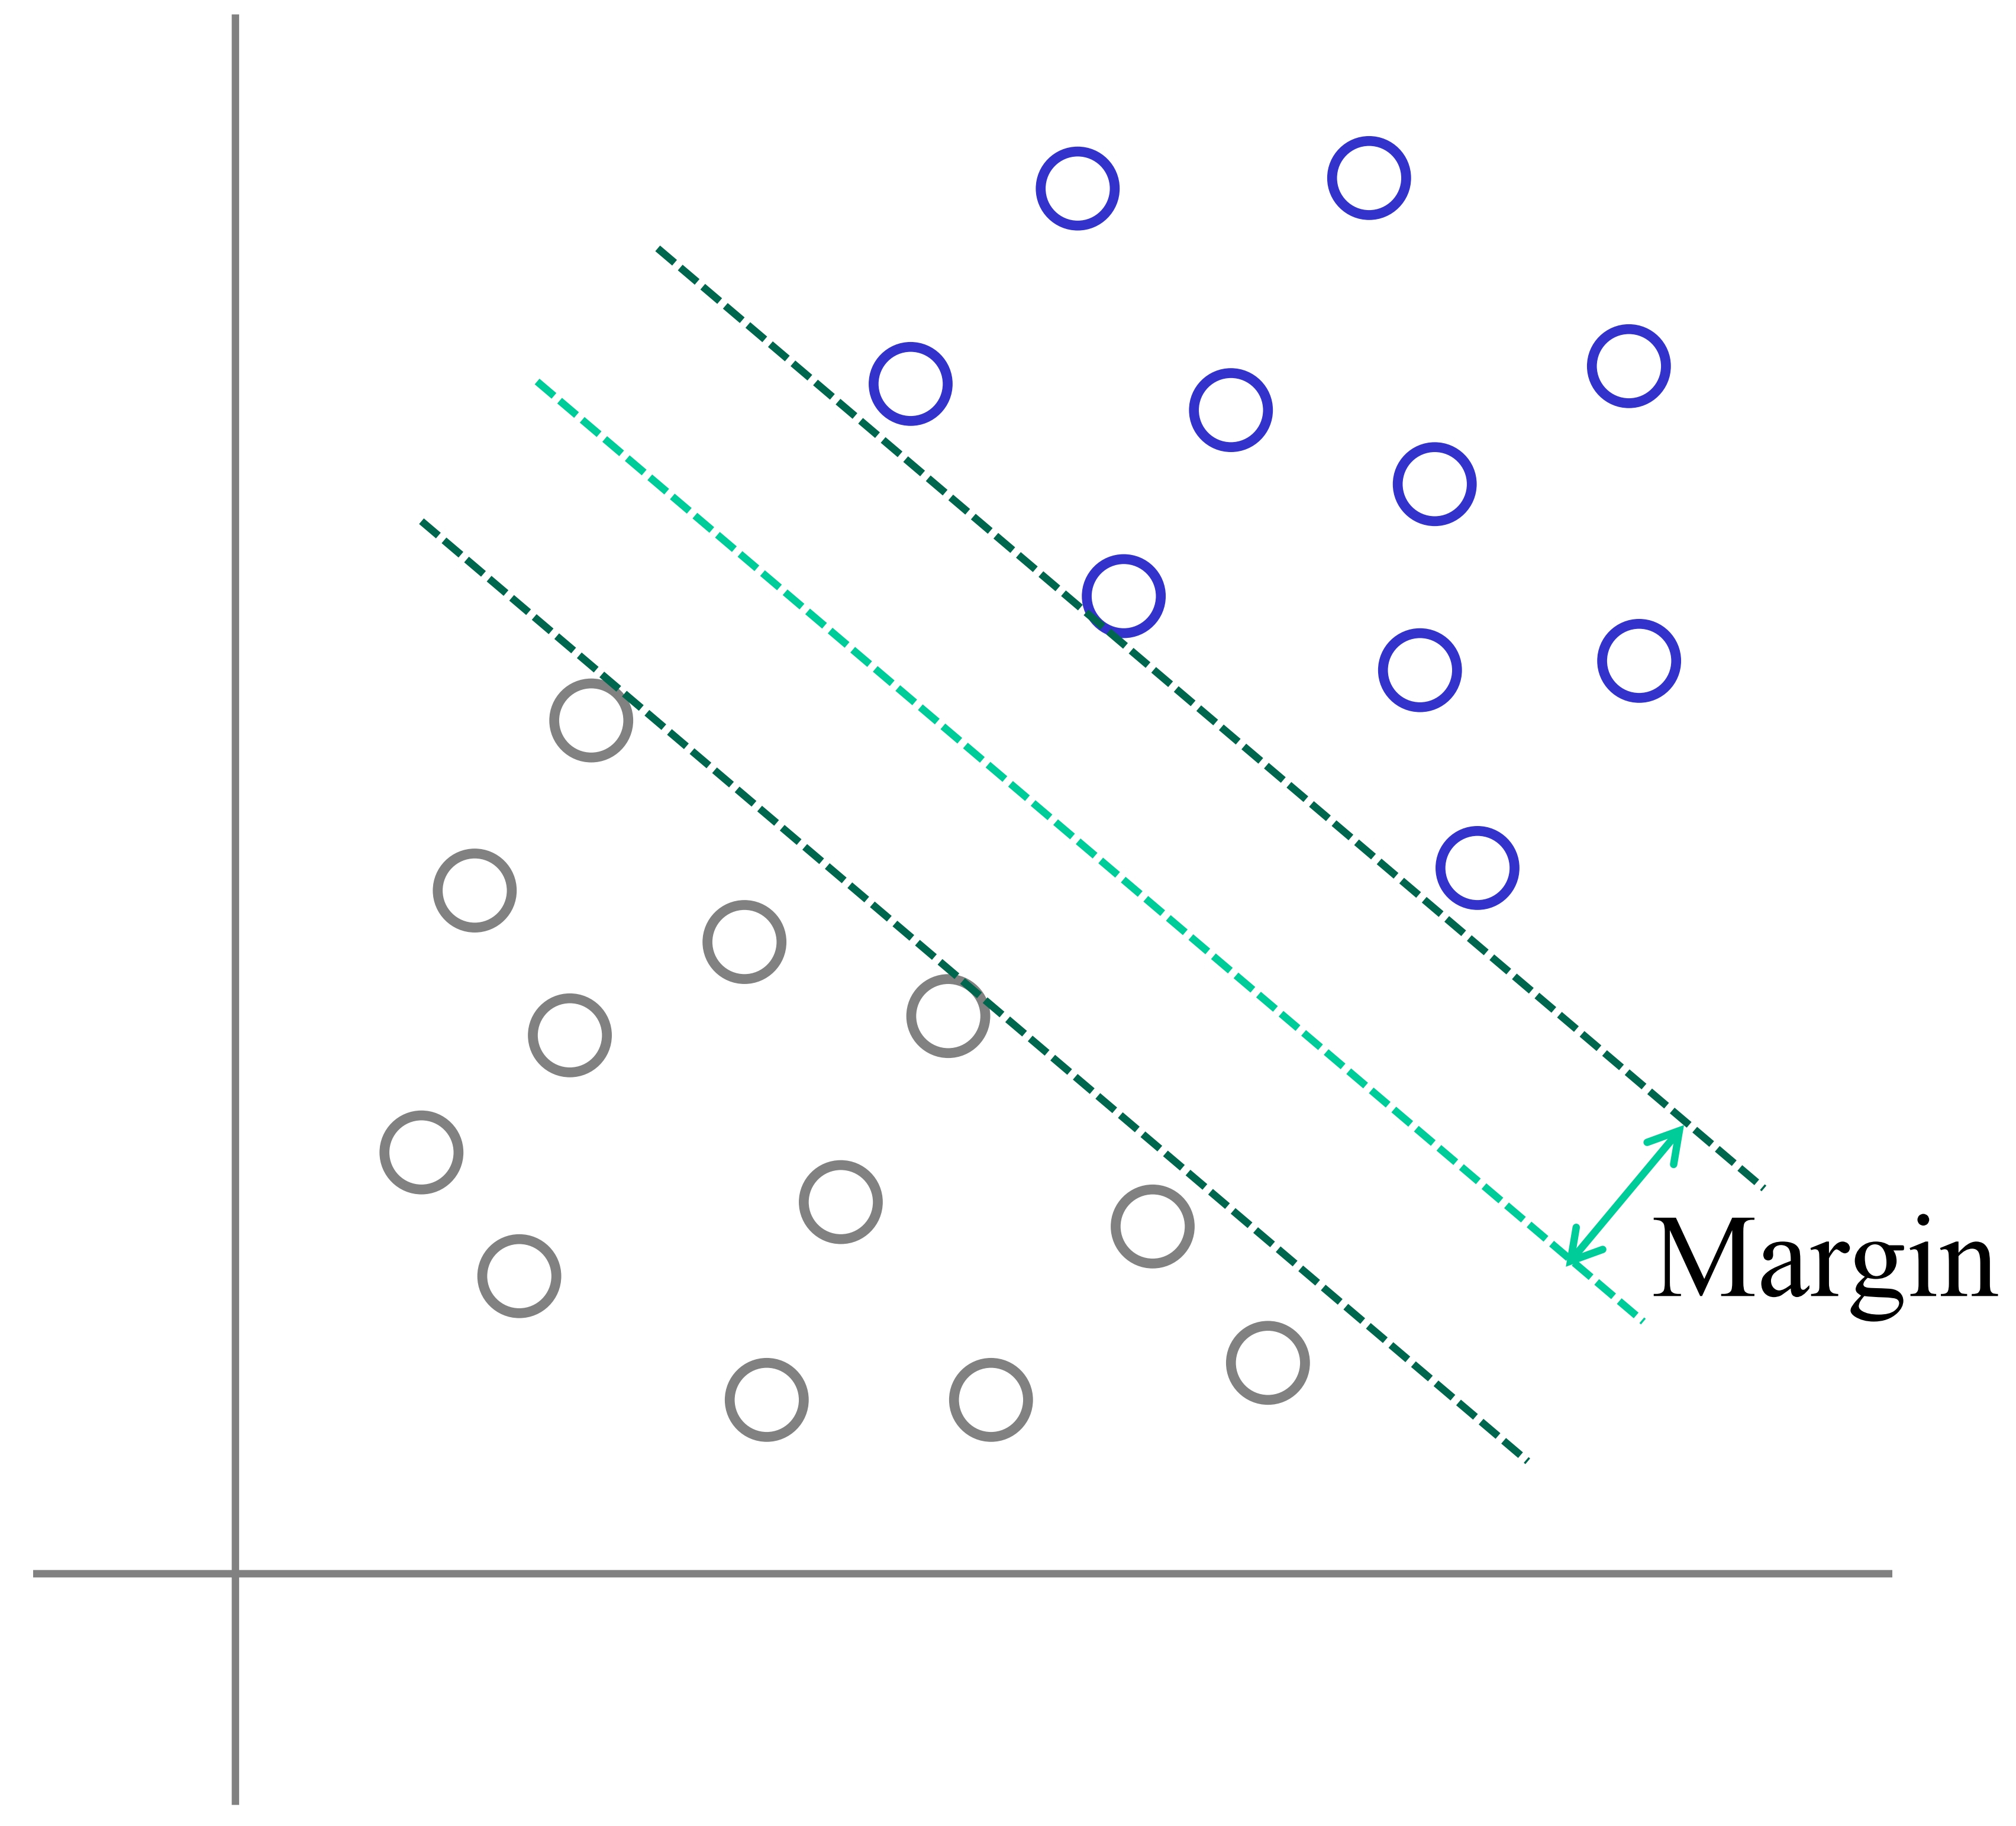
\includegraphics[width=0.6\linewidth]{fig8/lec86.jpg}
\end{center}
\end{frame}


% 7
\begin{frame}[c]
\frametitle{But the maximum margin hyperplane generalizes the best to new data}
\begin{itemize}
\item According to computational learning theory
\item Also known as statistical learning theory
\item We won't get into the details of that
\item Recall from the perceptron convergence proof
		\begin{itemize}
		\item We assumed the existance of a best hyperplane $\bm{w}_0$
		\item Which provided the maximum margin $\bm{\alpha}$
		\item Such that $d_p\bm{w}_0^T\bm{x}_p\leqslant{}\alpha$𝛼 for all training points 𝑝$p$
		\end{itemize}
\item The SVM actually finds this hyperplane
\end{itemize}

\end{frame}



% 8
\begin{frame}[c]
\frametitle{The maximum margin only depends on certain points, the support vectors}
\begin{center}
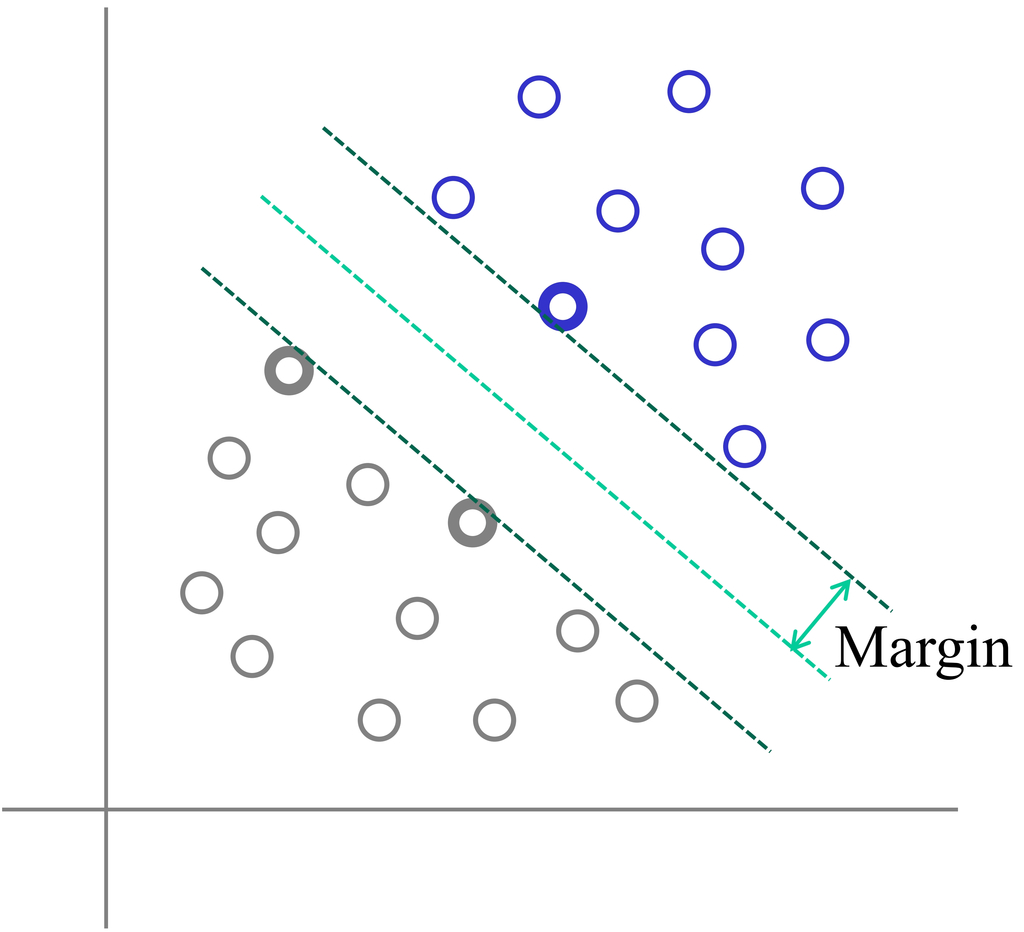
\includegraphics[width=0.7\linewidth]{fig8/lec88.jpg}
\end{center}
\end{frame}

% 9
\begin{frame}[c]
\frametitle{The maximum margin only depends on certain points, the support vectors}
\begin{center}
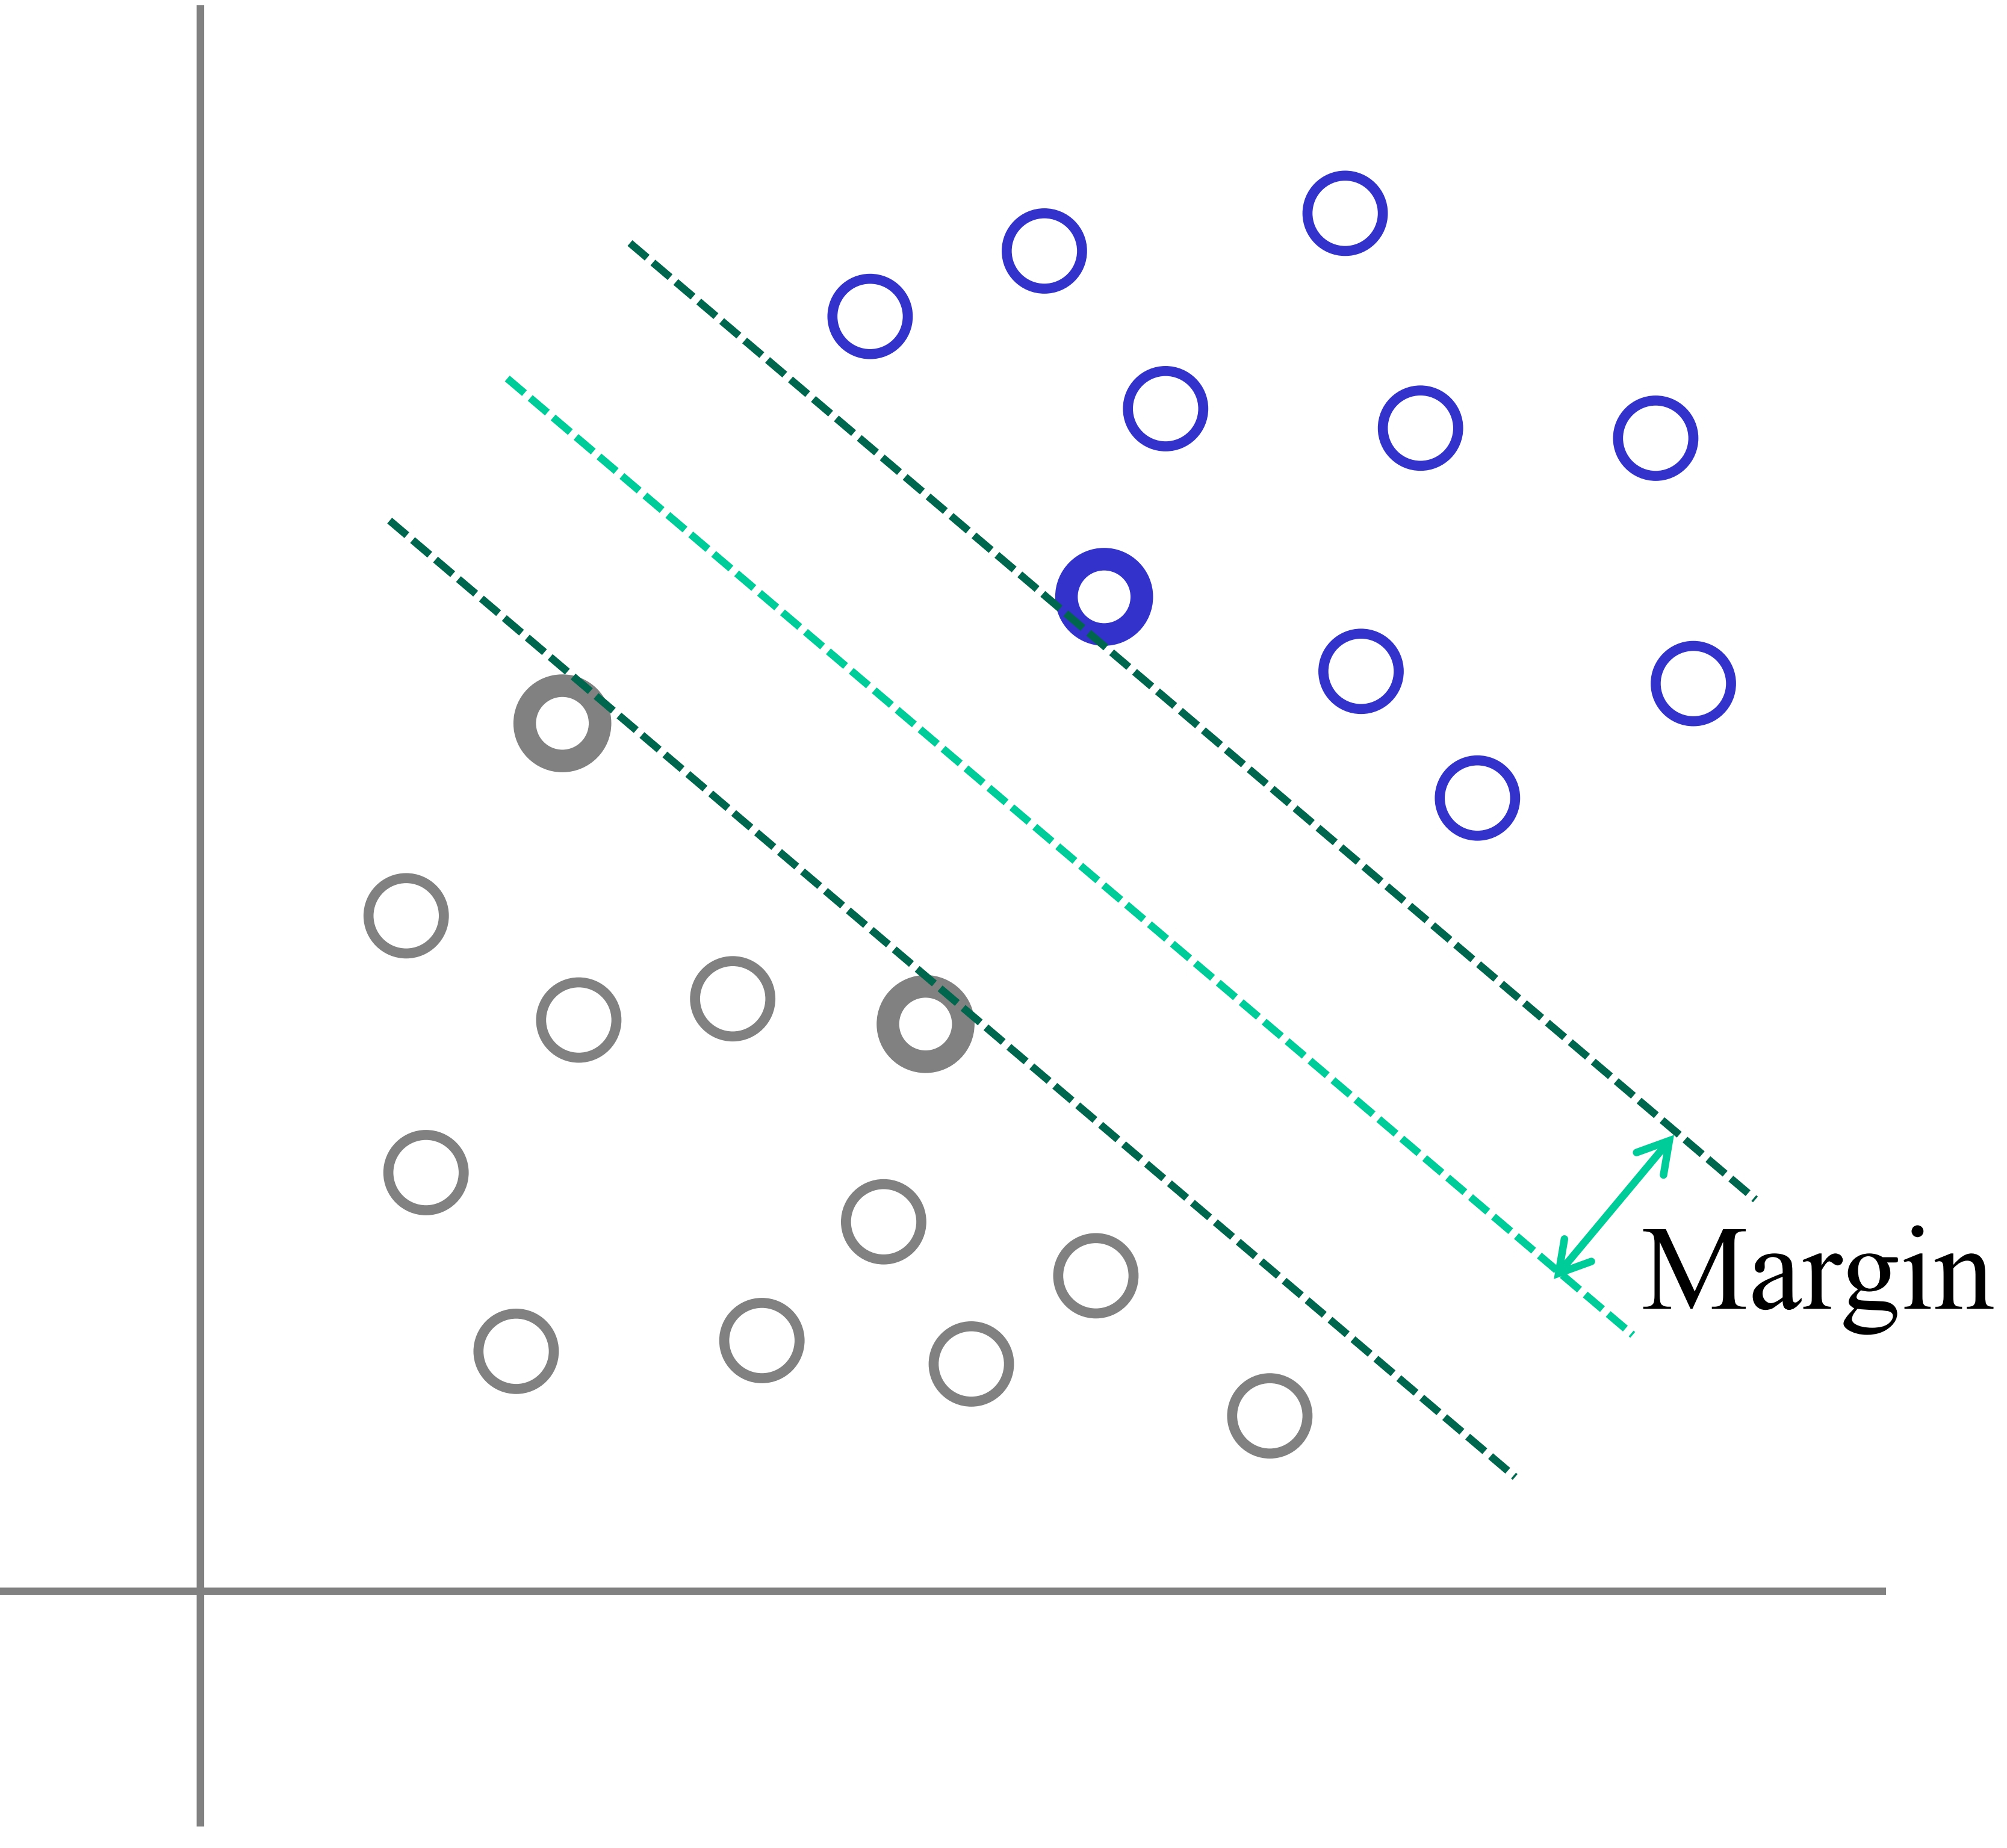
\includegraphics[width=0.7\linewidth]{fig8/lec89.jpg}
\end{center}
\end{frame}


% 10
\begin{frame}[c]
\frametitle{The maximum margin only depends on certain points, the support vectors}
\begin{center}
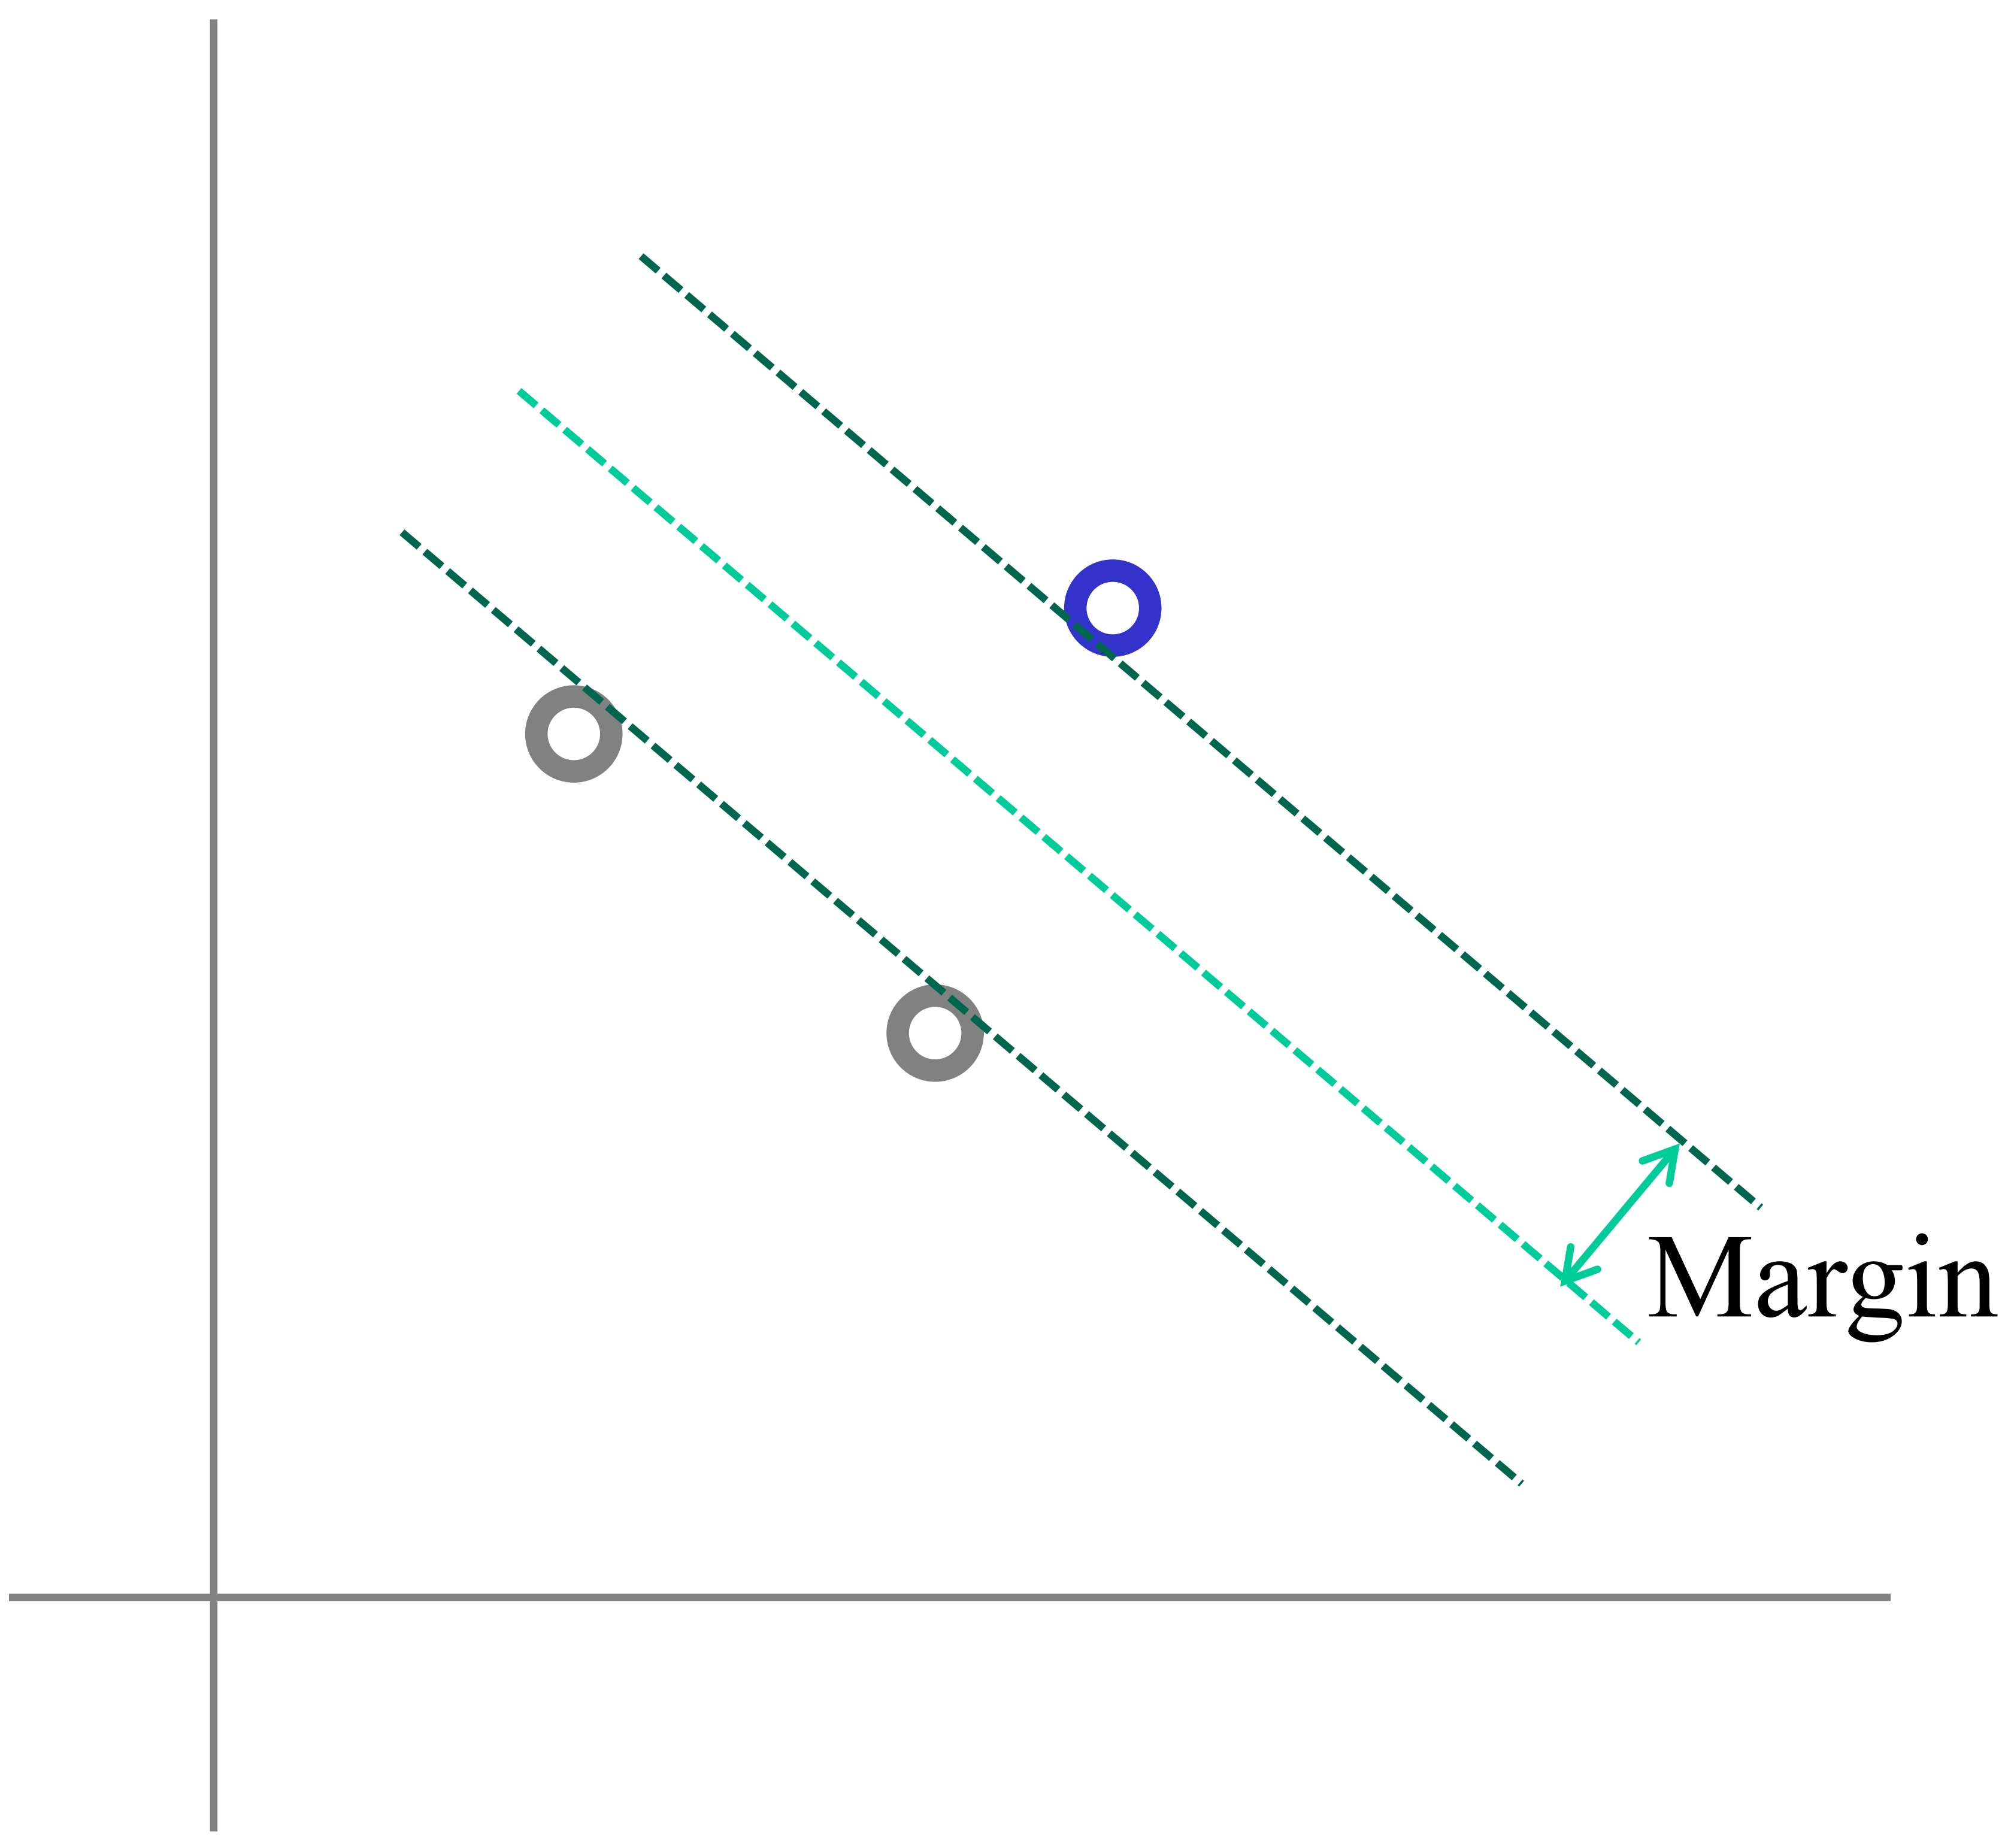
\includegraphics[width=0.7\linewidth]{fig8/lec810.jpg}
\end{center}
\end{frame}


% 11
\begin{frame}[c]
\frametitle{Maximum margin problem}
\begin{itemize}
\item  Given a set of data from two classes $\{\bm{x}_p,d_p\}$
		\begin{itemize}
		\item $x_p\in \mathbb{R}^D$ and $d_p\in\{-1,1\}$
		\item Assume the classes are linearly separable for now
		\end{itemize}
\item Find the hyperplane that separates them
		\begin{itemize}
		\item with maximum margin
		\end{itemize}
\item Equation of general linear discriminant function
\[y(\bm{x})=\bm{w}^T\bm{x}+b\]

\item Find $\bm{w}$ and 𝑏$b$ that give maximum margin
\item How can we quantify margin?
\end{itemize}

\end{frame}



% 12
\begin{frame}[c]
\frametitle{$\bm{w}$ is perpendicular to the hyperplane, $b$ defines its distance from the origin}
\begin{center}
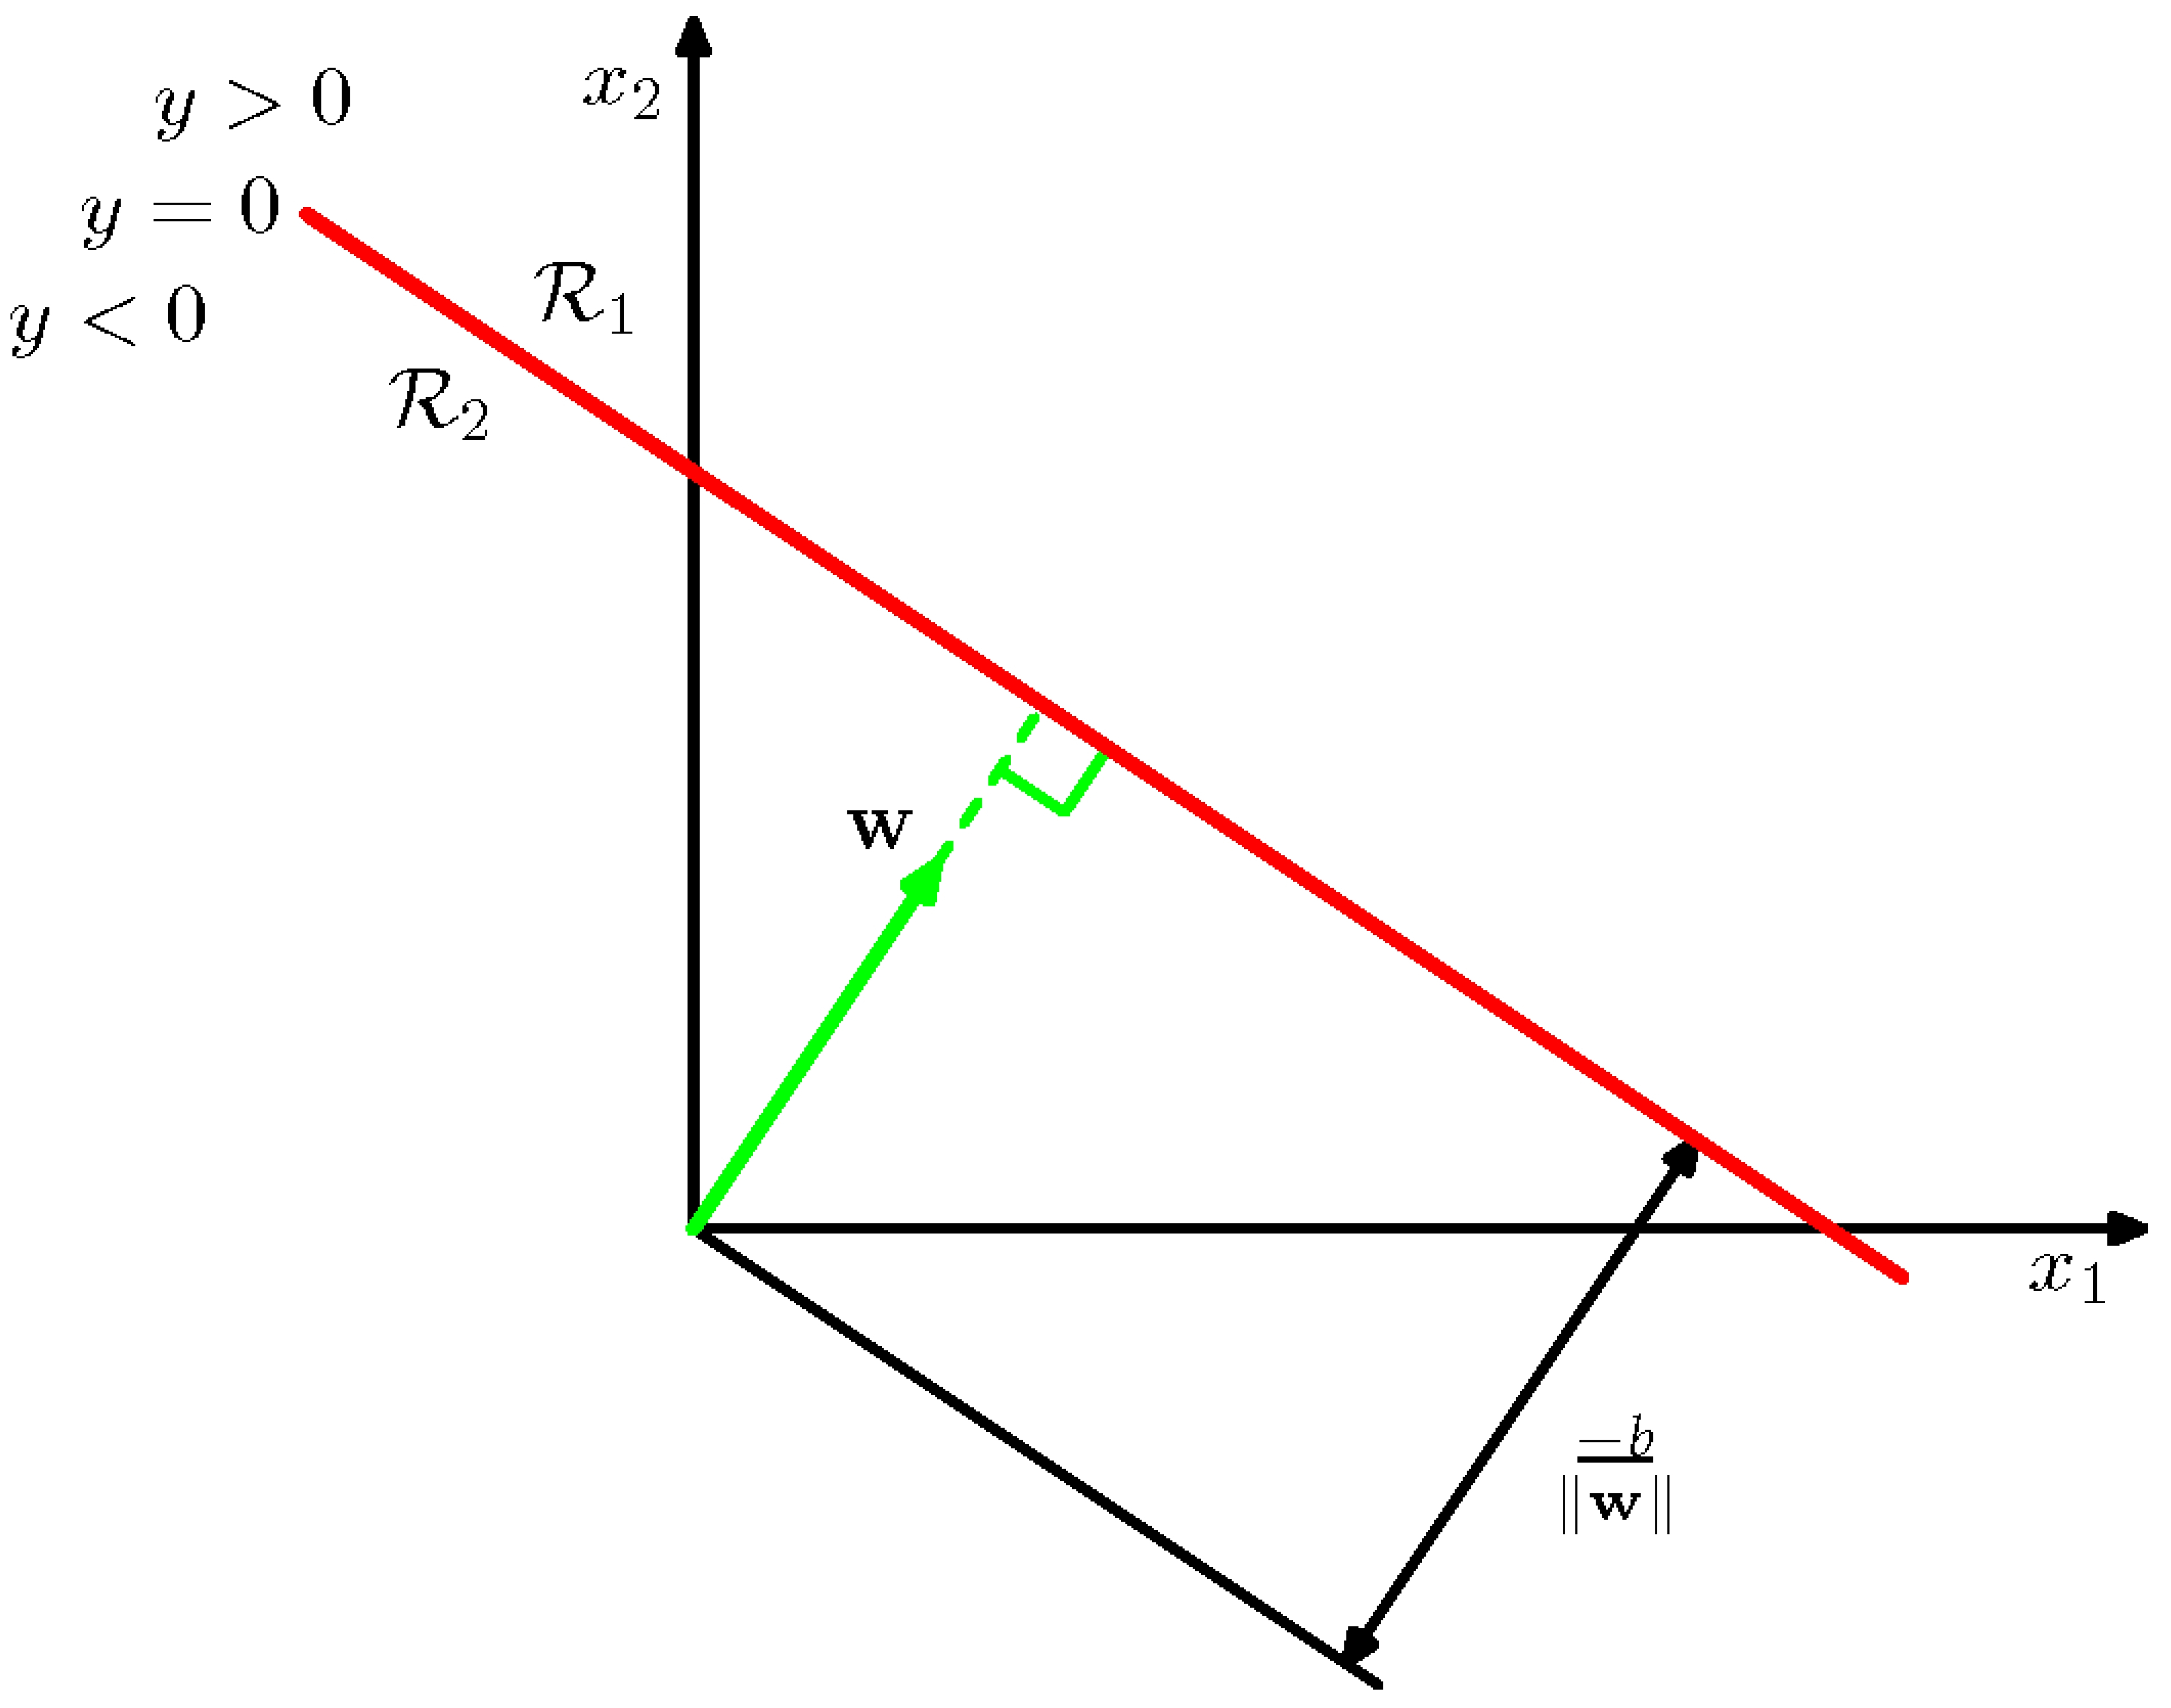
\includegraphics[width=0.7\linewidth]{fig8/lec812.jpg}
\end{center}
\end{frame}


% 13
\begin{frame}[c]
\frametitle{$\bm{w}$ is perpendicular to the hyperplane}
\begin{itemize}
\item Consider two points on the hyperplane $\bm{x}_A$ and $\bm{x}_B$
\item Then $y(\bm{x}_A)=y(\bm{x}_B)=0$ by definition
\item So $0 =y(\bm{x}_A)− y(\bm{x}_B) = \bm{w}^T(\bm{x}_A-\bm{x}_B)$𝒙𝒙 𝐵𝐵 
\item $\bm{x}_A-\bm{x}_B$ is  a vector pointing along the hyperplane
\item So $\bm{w}$ is perpendicular to the hyperplane
\end{itemize}

\end{frame}





% 14
\begin{frame}[c]
\frametitle{$b$ defines the hyerplane's distance from the origin}
\begin{itemize}
\item Consider a general point $\bm{x}$
\item Its distance to the origin is $D=\dfrac{\bm{w}^Tx}{||\bm{w}||}$
\item If $\bm{x}$ is on the hyperplane, then $y(\bm{x})=0$
		\begin{itemize}
		\item So $\bm{w}^T x=-b$
		\end{itemize}
\item So the distance from the hyperplane to the origin is
\[
D=-\dfrac{b}{||\bm{w}||}
\]
\end{itemize}

\end{frame}



% 15
\begin{frame}[c]
\frametitle{$\bm{w}$ is perpendicular to the hyperplane, $b$ defines its distance from the origin}
\begin{center}
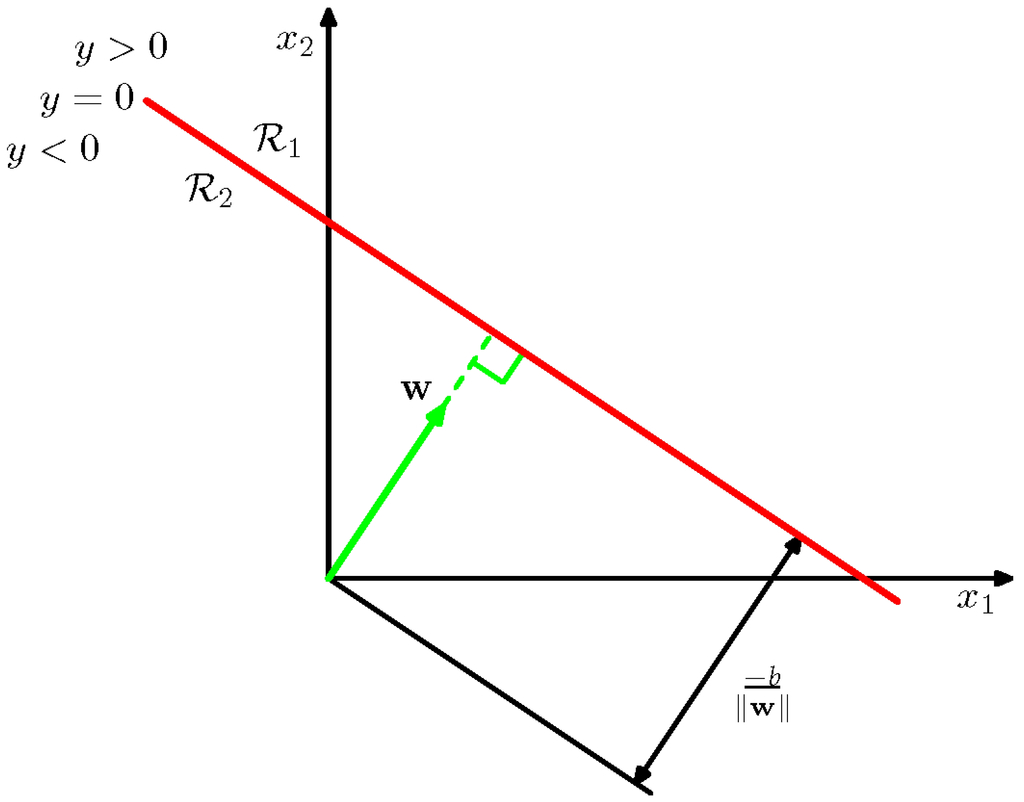
\includegraphics[width=0.7\linewidth]{fig8/lec815.jpg}
\end{center}
\end{frame}


% 16
\begin{frame}[c]
\frametitle{The distance from point $\bm{x}$𝒙to the hyperplane is 𝑦$y(\bm{x})/||\bm{w}||$}
\begin{center}
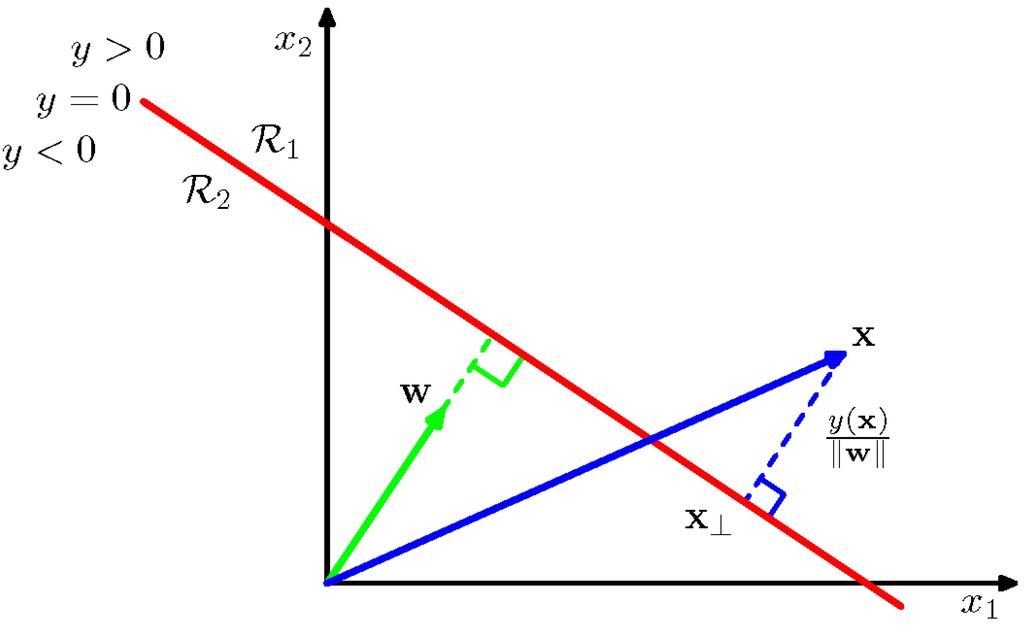
\includegraphics[width=0.7\linewidth]{fig8/lec816.jpg}
\end{center}
\end{frame}



% 17
\begin{frame}[c]
\frametitle{The distance from point $\bm{x}$𝒙to the hyperplane is 𝑦$y(\bm{x})/||\bm{w}||$}
\begin{itemize}
\item Consider a point $\bm{x}$ and its projection onto the hyperplane $\bm{x}_{\bot}$ so that $\bm{x}=\bm{x}_{\bot}+r\dfrac{\bm{x}}{||\bm{w}||}$𝑟𝑟
𝒘𝐀
\item We want to find $r$, the distance to the hyperplane
\item Multiply both sides by $\bm{w}^T$ and add $b$
\[
\bm{w}^T\bm{x}+b=
\bm{w}^T\bm{x}_{\bot} +b+r\dfrac{||\bm{w}||^2}{||\bm{w}||} 
\]
\[
y(\bm{x})=y(\bm{x}_{\bot})+r||\bm{w}||
\]
\[
r=\dfrac{y(\bm{x})}{||\bm{w}||}
\]
\end{itemize}
\end{frame}



% 18
\begin{frame}[c]
\frametitle{The distance from point $\bm{x}$𝒙to the hyperplane is 𝑦$y(\bm{x})/||\bm{w}||$}
\begin{center}
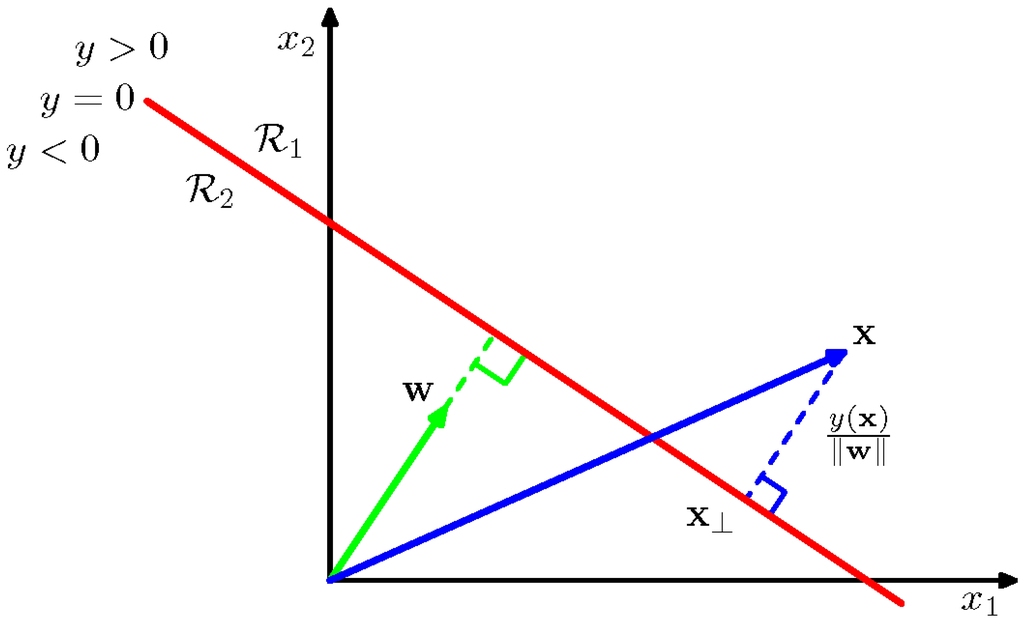
\includegraphics[width=0.7\linewidth]{fig8/lec818.jpg}
\end{center}
\end{frame}


% 19
\begin{frame}[c]
\frametitle{The maximum margin hyperplane is farthest from all of the data points}
\begin{center}
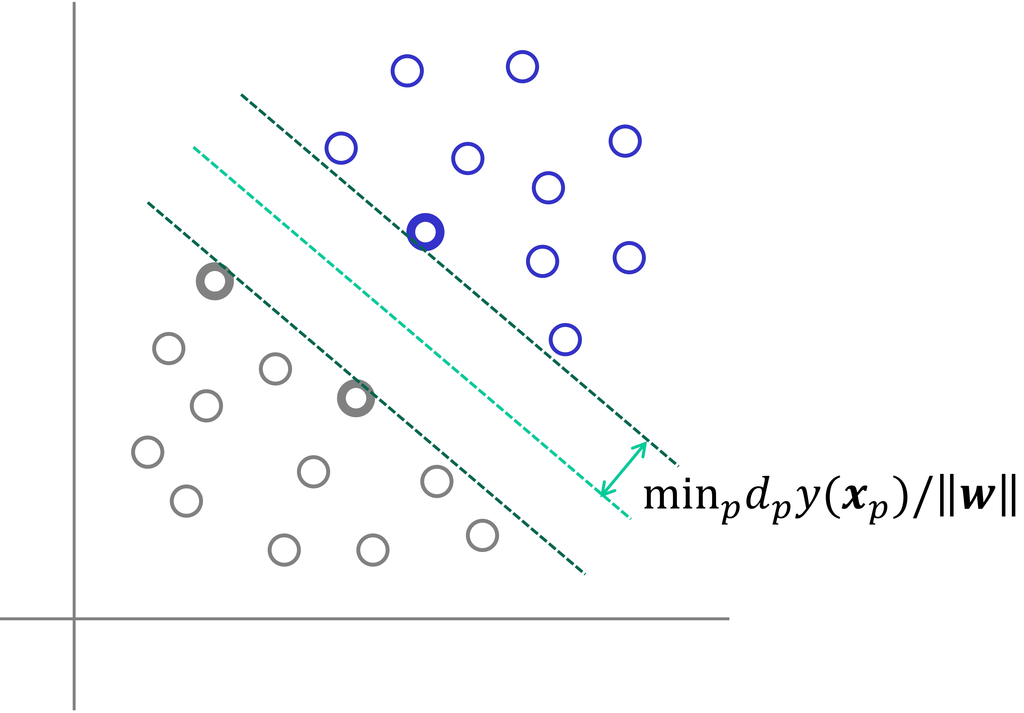
\includegraphics[width=0.7\linewidth]{fig8/lec819.jpg}
\end{center}
\end{frame}


% 20
\begin{frame}[c]
\frametitle{The maximum margin hyperplane is farthest from all of the data points}
\begin{itemize}
\item The margin is defined as
\[
\begin{array}{r@{~}l}
\alpha=&\min_pd_p\dfrac{y(\bm{x}_p)}{||\bm{w}||}\\
=&\dfrac{1}{||\bm{w}||}\min_pd_py(\bm{x}_p)
\end{array}
\]
\item We want to find $\bm{w}$ and 𝑏𝑏 that maximize the margin argmax$_{\bm{w},b}\dfrac{1}{||\bm{w}||} \min_pd_py(\bm{x}_p)$ 𝑑𝑑 𝑝𝑝 𝑦𝑦 𝒙𝒙 𝐀
\item Solving this problem is hard as it is written
\end{itemize}
\end{frame}

% 21
\begin{frame}[c]
\frametitle{We are free to choose a rescaling of $\bm{w}$}
\begin{itemize}
\item If we replace $\bm{w}$ by $a\bm{w}$ and $b$ with $ab$
\item Then the margin is unchanged
\[
\min\nolimits_pd_p\dfrac{a\bm{w}^T\bm{x}_p+ab}{a||\bm{w}||}=
\min\nolimits_pd_p
\dfrac{\bm{w}^T\bm{x}_p+b}{||\bm{w}||}
\]
\item So choose $a$ such that $\min_pd_p(a\bm{w}^T\bm{x}_p+ab)=1$
\item Which means that for all points 
\[
d_p(\bm{w}^T\bm{x}_p+b)\geqslant{}1
\]
\end{itemize}
\end{frame}


% 22
\begin{frame}[c]
\frametitle{Maximum margin constrained optimization problem}
\begin{itemize}
\item Then the maximum margin optimization becomes
\[
\begin{array}{c}
\text{argmax}_{\bm{w},b}\dfrac{1}{||\bm{w}||} \min_pd_py(\bm{x}_p)\\
= \text{argmax}_{\bm{w},b}\dfrac{1}{||\bm{w}||}
\end{array}
\]
\item With the constraints $d_p(\bm{w}^T\bm{x}_p+b)\geqslant{}1$
\end{itemize}
\end{frame}

% 23
\begin{frame}[c]
\frametitle{Maximum margin constrained optimization problem}
\begin{itemize}
\item Which is equivalent to \\
argmin$_{\bm{w},b}$ $\dfrac{1}{2}||\bm{w}||^2$~~~subject to $d_p(\bm{w}^T\bm{x}_p+b)\geqslant{}1$
\item This is a well studied type of problem
\begin{itemize}
\item A quadratic program with linear inequality constraints
\end{itemize}
\end{itemize}
\end{frame}



% 24
\begin{frame}[c]
\frametitle{Detour: Lagrange multipliers solve constrained optimization problems}
\begin{itemize}
\item Want to maximize a function $f(x_1,x_2)$
\item Subject to the equality constraint $g(x_1,x_2)= 0$
\item Could solve $g(x_1,x_2)= 0$ for $x_1$ in terms of $x_2$
\begin{itemize}
\item But that is hard to do in general (i.e., on computers)
\end{itemize}
\item Or could use Lagrange multipliers
\begin{itemize}
\item Which are easier to use in general (i.e., on computers)
\end{itemize}
\end{itemize}
\end{frame}


% 25
\begin{frame}[c]
\frametitle{Lagrange multipliers with general $\bm{x}$}
\begin{itemize}
\item In general, we can write
\[
\max\nolimits_x f(\bm{x})~\text{subject~to}~g(\bm{x})=0
\]
\item Constraint $g(\bm{x})= 0$ defines a $D− 1$ dimensional surface for $D$ dimensional $\bm{x}$
\end{itemize}
\end{frame}


% 26
\begin{frame}[c]
\frametitle{Example: Maximize $f(\bm{x})=1-x_1^2-x_2^2$ subject to $g(\bm{x})=x_1+x_2-1=0$}
\begin{center}
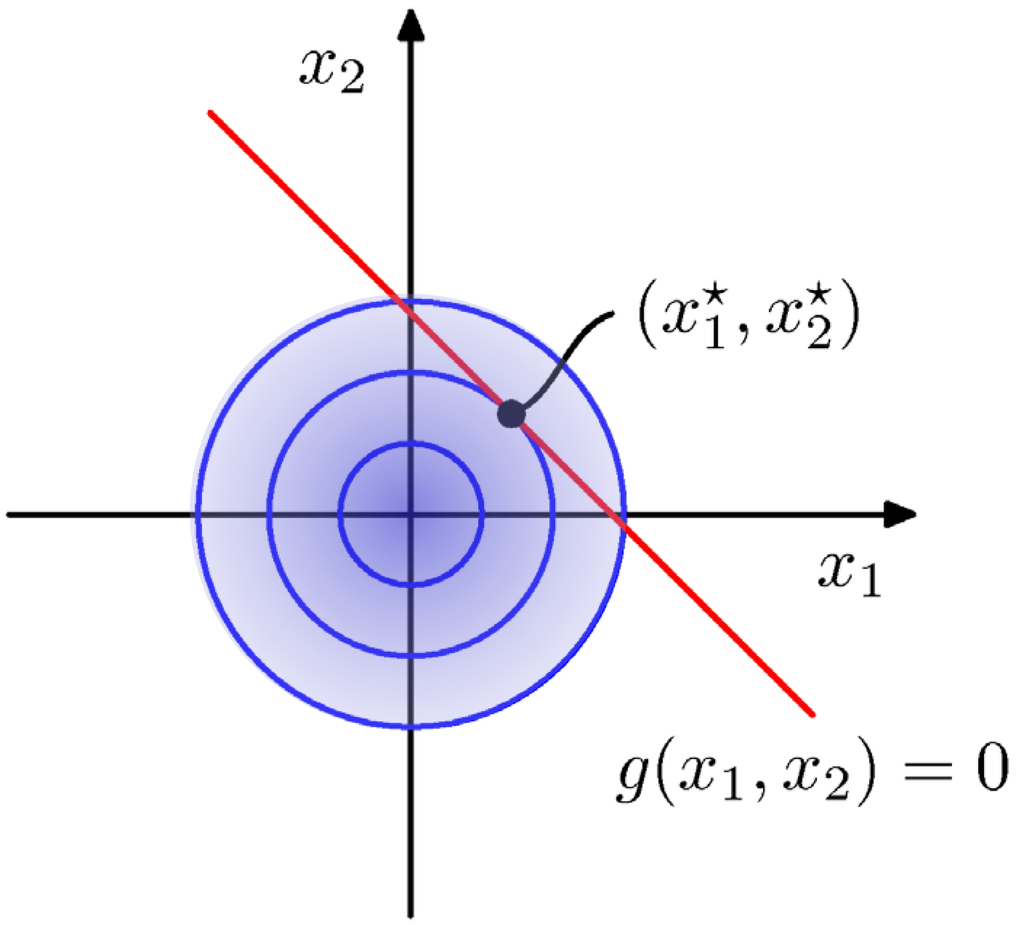
\includegraphics[width=0.7\linewidth]{fig8/lec826.jpg}
\end{center}
\end{frame}


% 27
\begin{frame}[c]
\frametitle{Gradients of $g$ and $f$ are orthogonal to surface at solution point}
\begin{center}
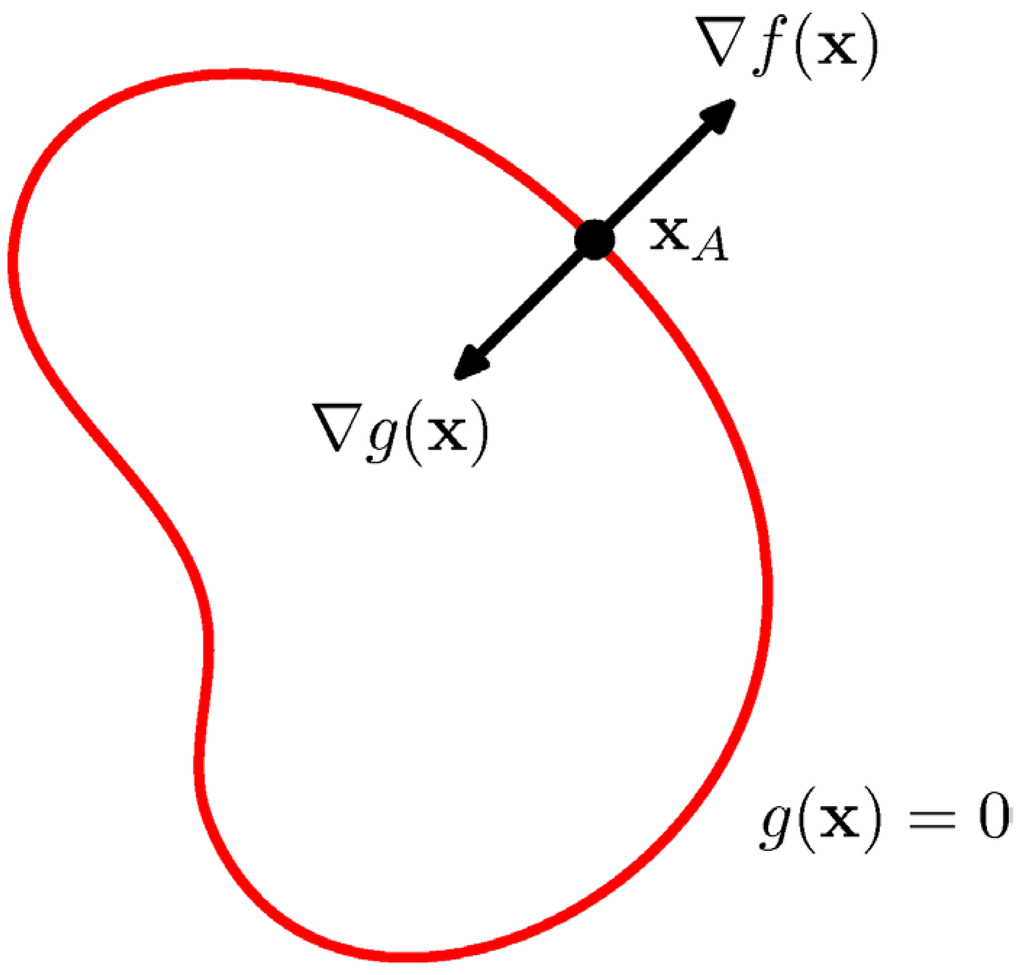
\includegraphics[width=0.65\linewidth]{fig8/lec827.jpg}
\end{center}
\end{frame}



% 28
\begin{frame}[c]
\frametitle{Gradients of $g$ and $f$ are orthogonal to surface at maximum of $f$}
\begin{itemize}
\item For $g$ because on all points on the surface $g(\bm{x})=0$
\item For $f$ because if it wasn't, you could move along the surface in the direction of the gradient to find a better maximum
\item Thus $\nabla f$ and $\nabla g$ are (anti-)parallel
\item And there must exist a scalar $\lambda$ such that
\[
\nabla f+\lambda \nabla g=0
\]
\end{itemize}
\end{frame}

% 29
\begin{frame}[c]
\frametitle{The Lagrangian function captures the constraints on 𝑥𝑥 and on the gradients}
\[
L(\bm{x},\lambda)=f(\bm{x})+\lambda g(\bm{x})
\]
\begin{itemize}
\item Setting gradient of $L$ with respect to $\bm{x}$ to 0 gives
\[
\nabla f+\lambda \nabla g=0
\]
\item Setting partial of $L$ with respect to $\lambda$ to 0 gives
\[
g(\bm{x})=0
\]
\item Thus stationary points of $L$ solve the constrained optimization problem
\end{itemize}
\end{frame}



% 30
\begin{frame}[c]
\frametitle{Example: Maximize $f(\bm{x})=1-x_1^2-x_2^2$ subject to $g(\bm{x})=x_1+x_2-1=0$}
\begin{center}
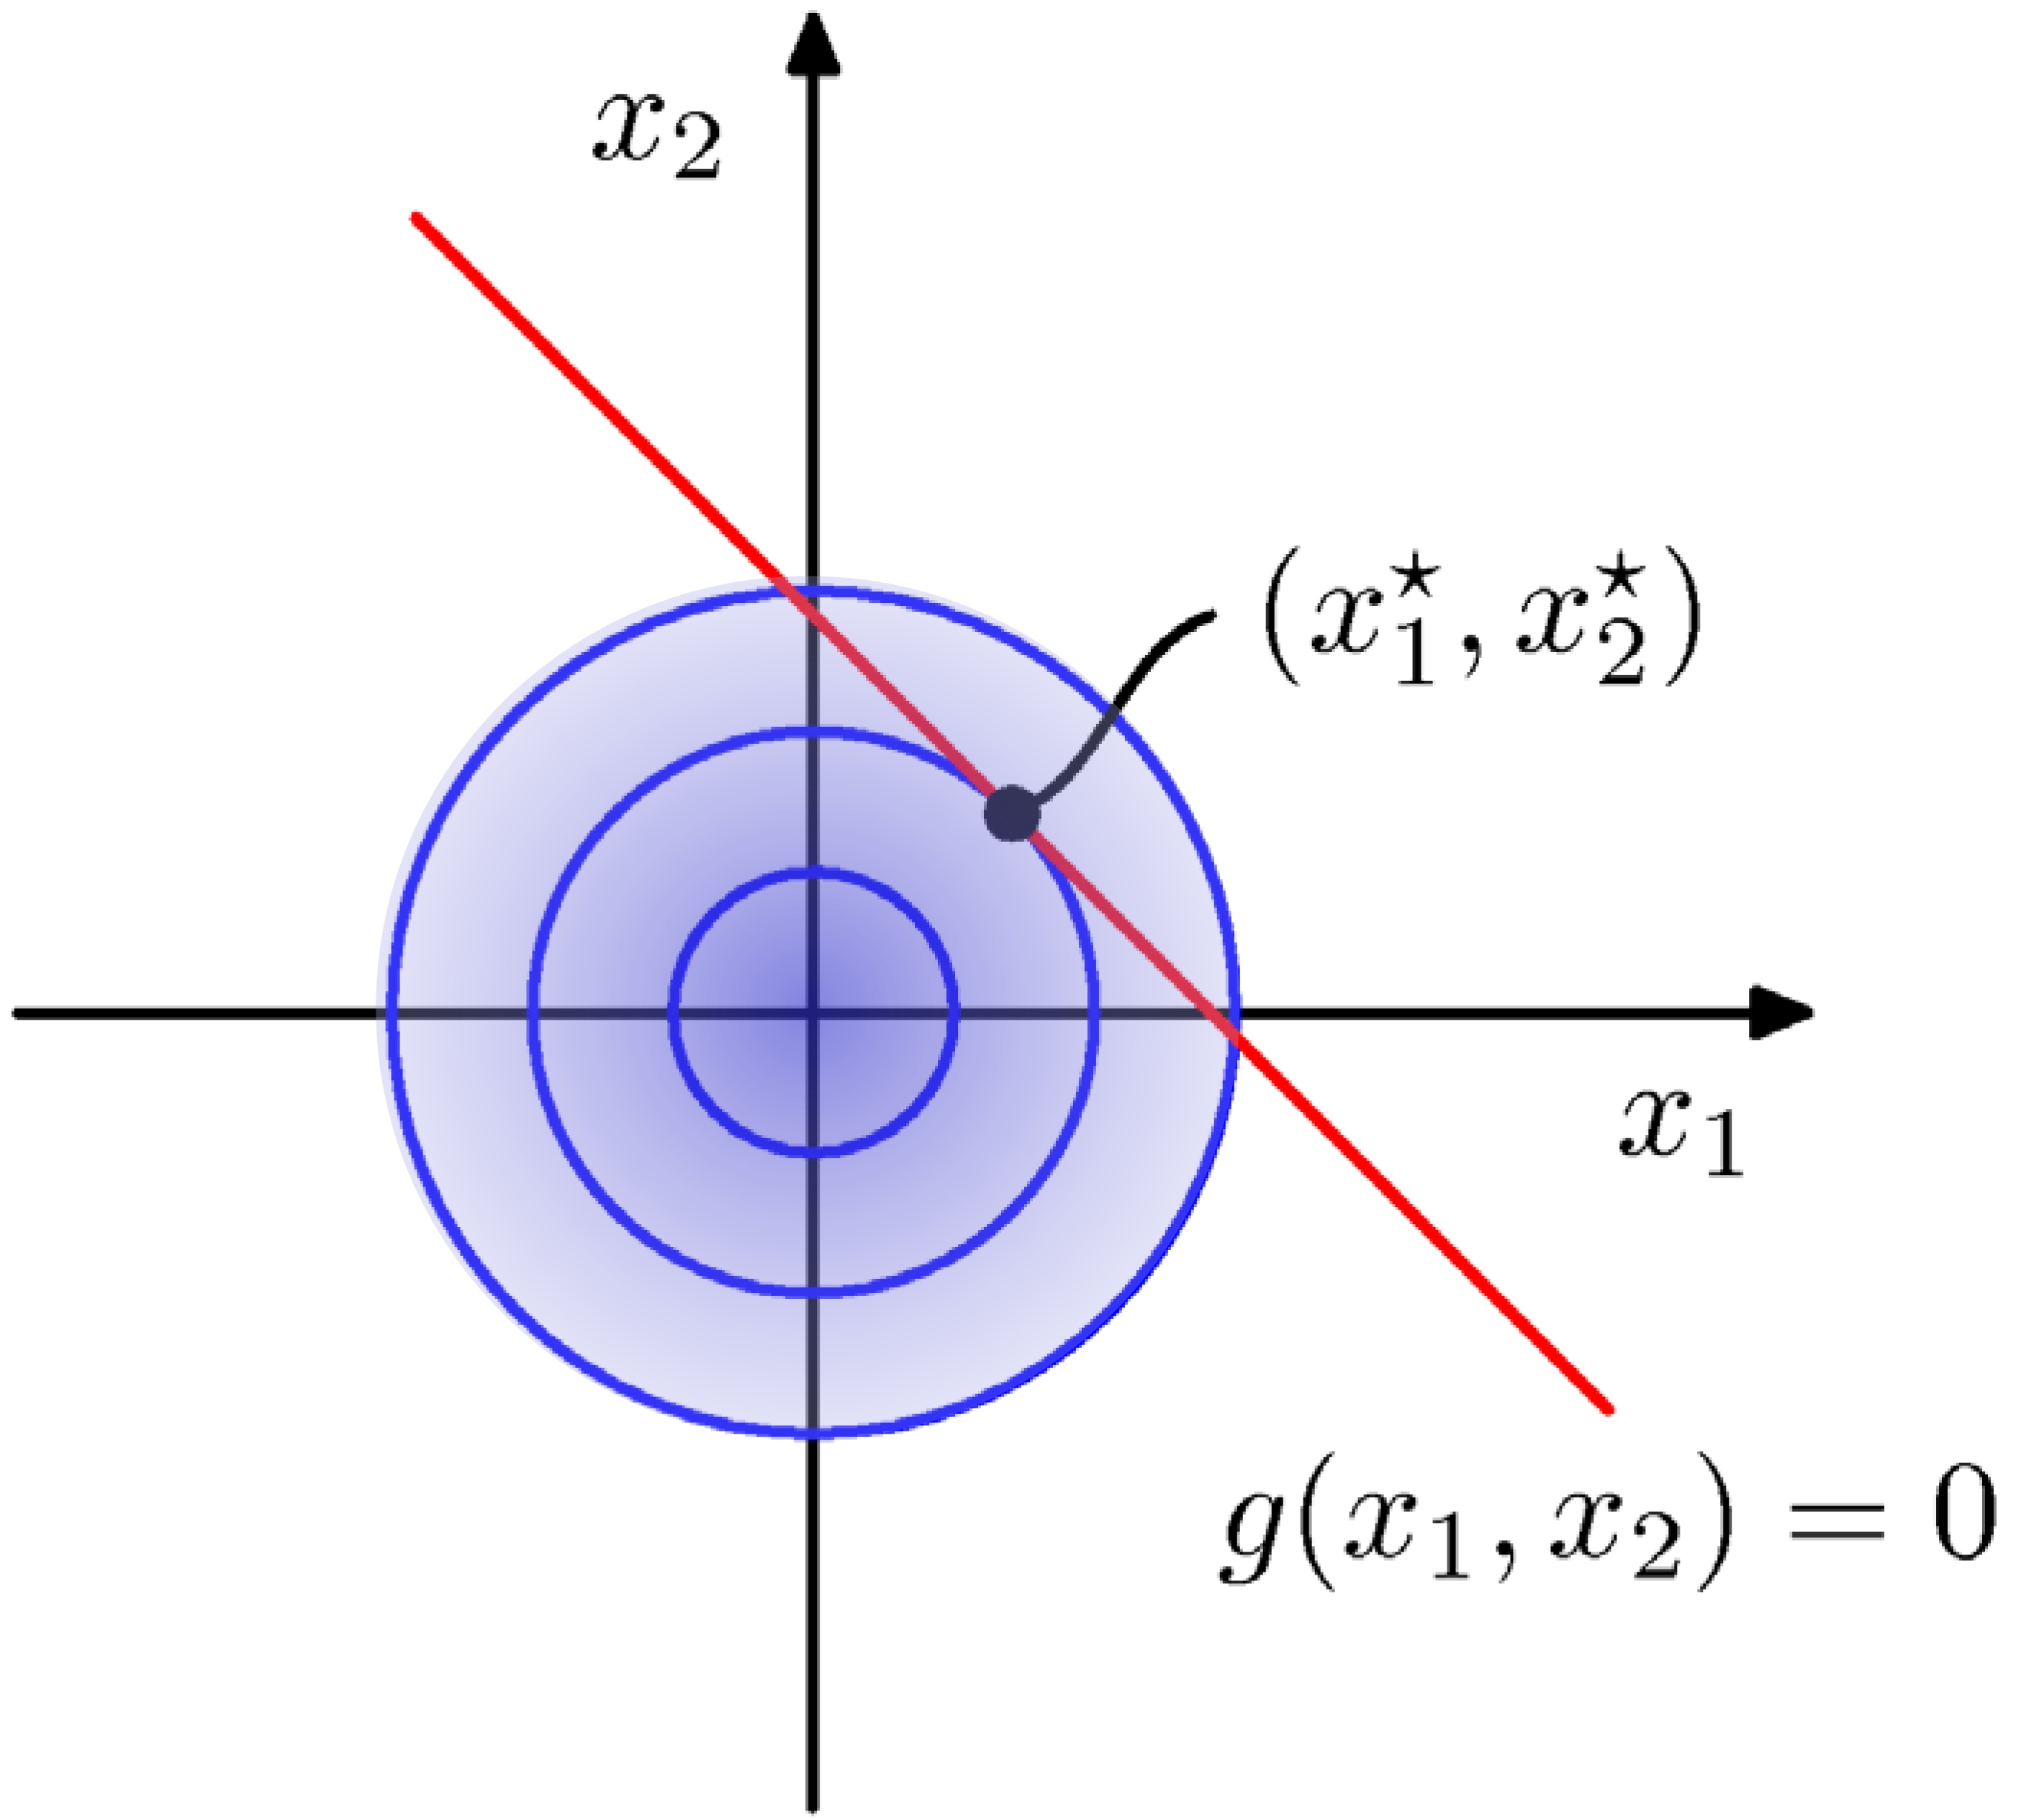
\includegraphics[width=0.65\linewidth]{fig8/lec830.jpg}
\end{center}
\end{frame}


% 31
\begin{frame}[c]
\frametitle{Example: Maximize $f(\bm{x})=1-x_1^2-x_2^2$ subject to $g(\bm{x})=x_1+x_2-1=0$}
\begin{itemize}
\item So the Lagrangian function is
\[
\begin{array}{r@{~}l}
L(\bm{x},\lambda)=&f(\bm{x})+\lambda g(\bm{x})\\
=&1-x_1^2-x_2^2+\lambda(x_1+x_2-1)
\end{array}
\]
\item The conditions for $L$ to be stationary are
\[
\begin{array}{r@{~}l}
\partial L/\partial x_1=-2x_1+\lambda=0\\
\partial L/\partial x_2=-2x_2+\lambda=0\\
\partial L/\partial \lambda=x_1+x_2-1=0\\
\end{array}
\]
\item Can solve to find $\lambda=1,x_1=x_2=\dfrac{1}{2}$
\end{itemize}
\end{frame}


% 32
\begin{frame}[c]
\frametitle{Lagrange multipliers can also be used with inequality constraints $g(\bm{x})\geqslant{}0$}
\begin{center}
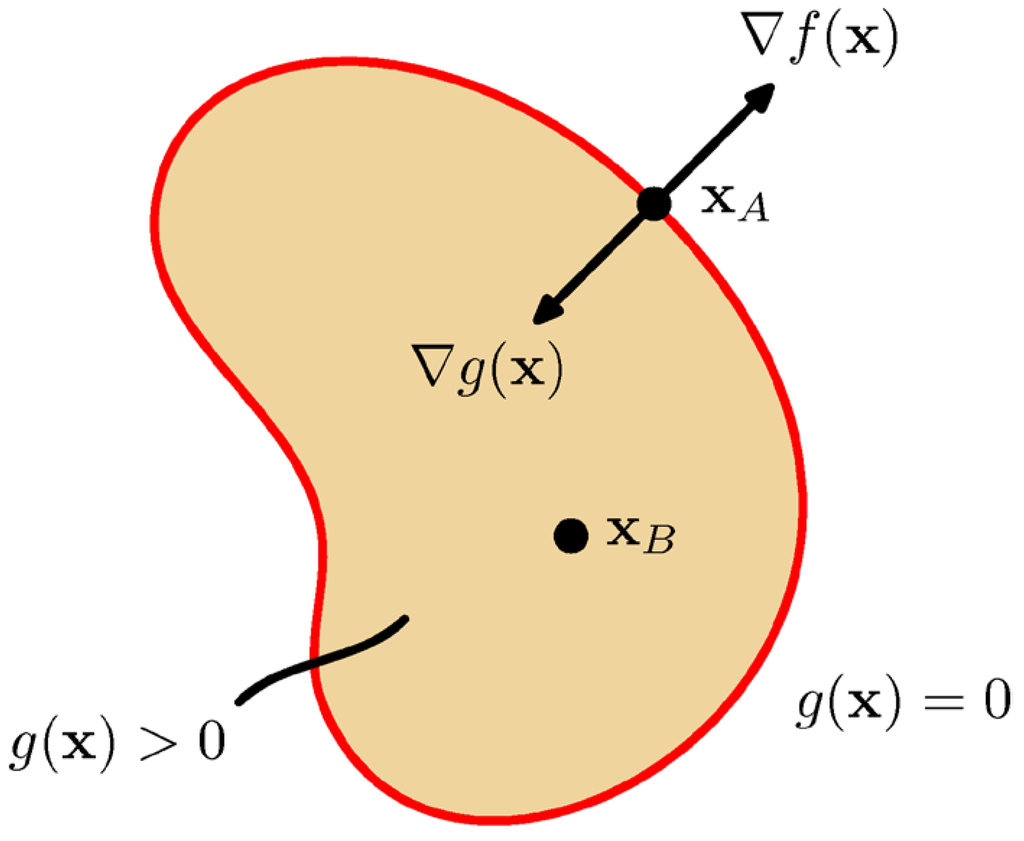
\includegraphics[width=0.65\linewidth]{fig8/lec832.jpg}
\end{center}
\end{frame}


% 33
\begin{frame}[c]
\frametitle{Lagrange multipliers can also be used with inequality constraints $g(\bm{x})\geqslant{}0$}
\begin{itemize}
\item Now two kinds of solutions:
\item If $g(\bm{x})> 0$, then the solution only depends on $f(\bm{x})$
\begin{itemize}
\item Inside constraint surface with $\nabla f= 0$
\item Stationary point of $L(\bm{x},𝜆\lambda)$ with $\lambda= 0$
\item Constraint $g(\bm{x})$ is said to be inactive
\end{itemize}
\item If $g(x)= 0$, then same as before (with equality constraint)
\begin{itemize}
\item On boundary of constraint surface with $\nabla f$ pointing out
\item Stationary point of $L(\bm{x},\lambda)$ with $\lambda> 0$
\item Constraint $g(\bm{x})$ is said to be active
\end{itemize}

\end{itemize}
\end{frame}


% 34
\begin{frame}[c]
\frametitle{Lagrange multipliers can also be used with inequality constraints $g(\bm{x})\geqslant{}0$}
\begin{itemize}
\item In either case, $\lambda g(\bm{x})=0$
\item Thus maximizing $f(\bm{x})$ subject to $g(\bm{x})\geqslant{}0$ is obtained by optimizing $L(\bm{x},\lambda)$ WRT $\bm{x}$ and $\lambda$ subject to
\[
\begin{array}{c}
g(\bm{x})\geqslant{}0\\
\lambda\geqslant{}0\\
\lambda g(\bm{x})=0
\end{array}
\]
\item These are known as the Karush-Kuhn-Tucker (KKT) conditions
\end{itemize}
\end{frame}


% 35
\begin{frame}[c]
\frametitle{Example: Maximize $f(\bm{x})=1-x_1^2-x_2^2$ subject to $g(\bm{x})=x_1+x_2-1\geqslant{}0$}
\begin{center}
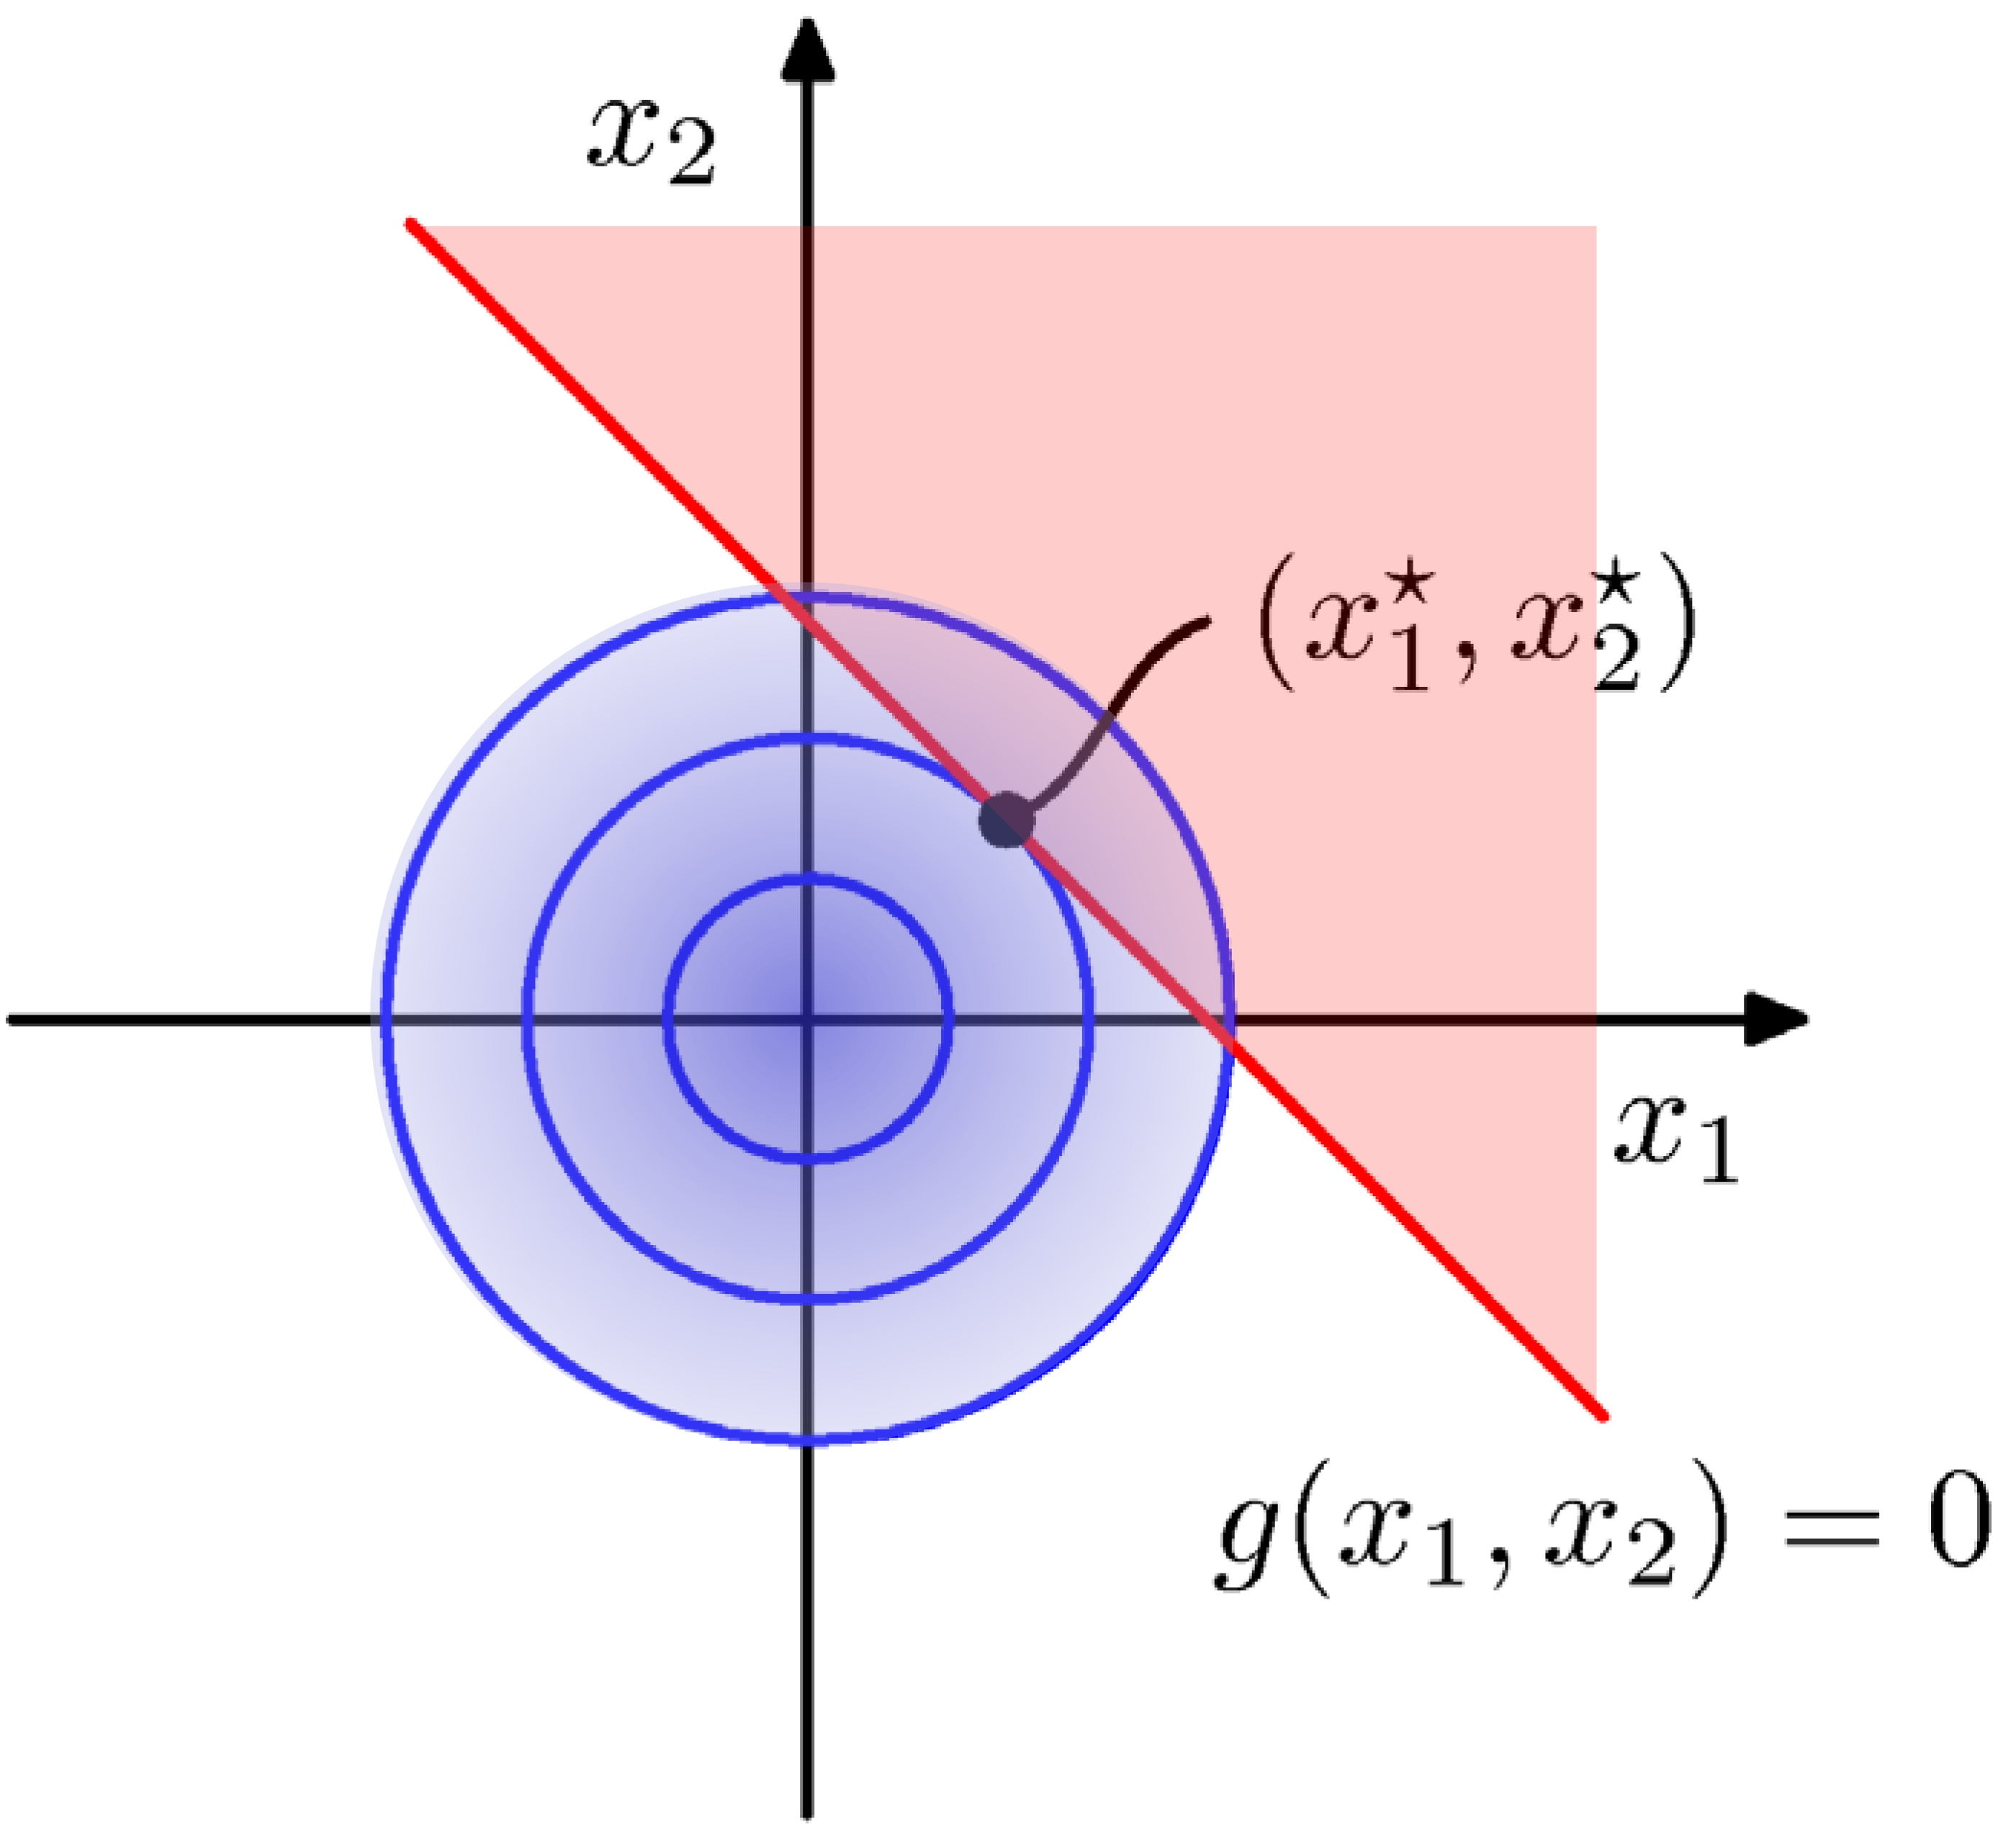
\includegraphics[width=0.65\linewidth]{fig8/lec835.jpg}
\end{center}
\end{frame}


% 36
\begin{frame}[c]
\frametitle{Example: Maximize $f(\bm{x})=1-x_1^2-x_2^2$ subject to $g(\bm{x})=x_1+x_2-1\geqslant{}0$}
\begin{itemize}
\item So the Lagrangian function is 
\[
L(\bm{x},\lambda)=1-x_1^2-x_2^2+\lambda(x_1+x_2-1)
\]
\item The conditions for $L$ to be stationary are 
\[
\begin{array}{r@{~}l}
\partial L/\partial x_1=-2x_1+\lambda=0\\
\partial L/\partial x_2=-2x_2+\lambda=0\\
\partial L/\partial \lambda=x_1+x_2-1=0\\
\end{array}
\]
\item Can solve to find $\lambda=1,x_1=x_2=\dfrac{1}{2}$
\begin{itemize}
\item Which still satisfies KKT conditions
\end{itemize}
\end{itemize}
\end{frame}


% 37
\begin{frame}[c]
\frametitle{Example: Maximize $f(\bm{x})=1-x_1^2-x_2^2$ subject to $g(\bm{x})=-x_1-x_2-1\geqslant{}0$}
\begin{center}
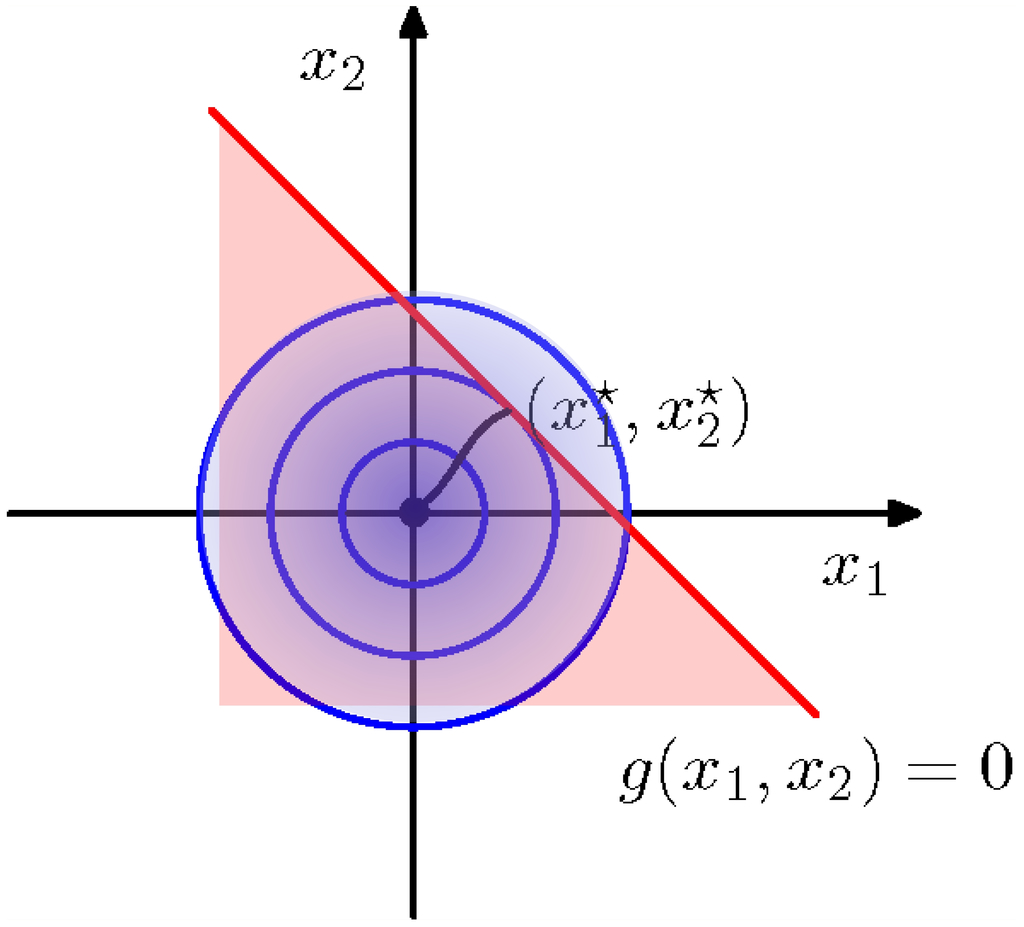
\includegraphics[width=0.65\linewidth]{fig8/lec837.jpg}
\end{center}
\end{frame}


% 38
\begin{frame}[c]
\frametitle{Example: Maximize $f(\bm{x})=1-x_1^2-x_2^2$ subject to $g(\bm{x})=-x_1-x_2-1\geqslant{}0$}
\begin{itemize}
\item So the Lagrangian function is 
\[
L(\bm{x},\lambda)=1-x_1^2-x_2^2+\lambda(-x_1-x_2+1)
\]
\item The conditions for $L$ to be stationary are 
\[
\begin{array}{r@{~}l}
\partial L/\partial x_1=-2x_1-\lambda=0\\
\partial L/\partial x_2=-2x_2-\lambda=0\\
\partial L/\partial \lambda=x_1+x_2-1=0\\
\end{array}
\]
\item Can solve to find $\lambda=-1$
\begin{itemize}
\item which does not satisfy KKT condition $\lambda \geqslant{}0$
\end{itemize}
\item Instead use unconstrained solution $x_1=x_2=0$
\begin{itemize}
\item which does satisfy KKT conditions
\end{itemize}
\end{itemize}
\end{frame}


% 39
\begin{frame}[c]
\frametitle{Multiple constraints each get their own Lagrange multiplier}
\begin{itemize}
\item Maximize $f(\bm{x})$ subject to $g_i(\bm{x})= 0$ and $h_j(x)\geqslant{}0$
\item Leads to the Lagrangian function
\[
L(\bm{x,\lambda,\mu})=f(\bm{x})+\sum_i \lambda_ig_i(\bm{x})+\sum_ju_jh_j(\bm{x})
\]
\item Still solve for $\nabla L(\bm{x,\lambda,\mu})= 0$
\item Trickier in general to figure out which $h_j(\bm{x})$ constraints should be active
\end{itemize}
\end{frame}



% 40
\begin{frame}[c]
\frametitle{Minimizing $f(\bm{x})$ with an inequality constraint requires a slightly different Lagrangi}
\begin{itemize}
\item Minimize WRT $\bm{x}$
\[
L(\bm{x},\lambda)=f(\bm{x})-\lambda g(\bm{x})
\]
\item Still subject to
\[
g(\bm{x})\geqslant{}0
\]
\end{itemize}
\end{frame}


% 41
\begin{frame}[c]
\frametitle{Summary of Lagrange multipliers with multiple inequality constraints}
\begin{itemize}
\item Goal: maximize $f(\bm{x})$ subject to $g_i(\bm{x})\geqslant{} 0$
\item Write down Lagrangian function
\[
L(\bm{x},\lambda)=f(x)+\sum_i\lambda_ig_i(\bm{x})
\]
\item Find points where $\nabla L(\bm{x},\lambda)= 0$
\item Keep points that satisfy constraints $g_x(\bm{x})\geqslant{}0$
\item Figure out which KKT conditions should be active
\begin{itemize}
\item Don't need to try all $2^I$ combinations for SVMs
\item Because $f(\bm{x})$ and $g(\bm{x})$ form a ``quadratic program''
\end{itemize}
\end{itemize}
\end{frame}

% 42
\begin{frame}[c]
\frametitle{Back to SVMs: Maximum margin solution is a fixed point of the Lagrangian function}
\begin{itemize}
\item Recall, the maximum margin hyperplane is

argmin$_{\bm{w},b} \dfrac{1}{2}||\bm{w}||^2$ subject to $d_p(\bm{w}^T \bm{x}_p+b)\geqslant{}1$
\begin{itemize}
\item Minimization of a quadratic function subject to multiple linear inequality constraints
\end{itemize}
\item Will use Lagrange multipliers, $a_p$, to write Lagrangian function

$L(\bm{w},b,\bm{a})=\dfrac{1}{2}||\bm{w}||^2-\sum\limits_pa_p(d_p(\bm{w}^T\bm{x}_p+b)-1)$
\item Note that $\bm{x}_p$ and $d_p$ are fixed for the optimization
\end{itemize}
\end{frame}











% % 9
% \begin{frame}[c]
% \frametitle{Example orthogonal complete basis: Chebyshev polynomials}
% \begin{equation*}
% \begin{array}{c}
% T_0(x)=1\qquad
% T_1(x)=1\qquad
% T_{n+1}(x)=2xT_n(x)-T_{n-1}(x)\\[2mm]
% {\rm Complete~on~the~interval}~[0,1]\\[2mm]
% T_2(x)=2x^2-1\qquad
% T_3(x)=4x^3-3x\quad {\rm etc.}
% \end{array}
% \end{equation*}
% \begin{center}
% 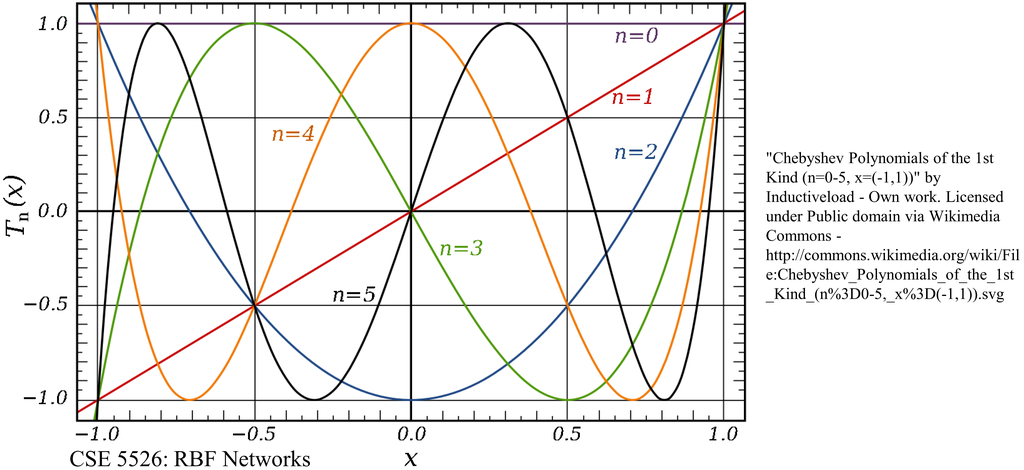
\includegraphics[width=0.85\linewidth]{fig/lec79.jpg}
% \end{center}
% \end{frame}

% % 10
% \begin{frame}[c]
% \frametitle{Radial basis functions}
% \begin{itemize}
% \item 𝑖A radial basis function (RBF) is a basis function of the form $\varphi_j(\mathbf{x})=\varphi(||\mathbf{x}-\mathbf{\mu}_j||)$
% 𝑤𝑤
		% \begin{itemize}
		% \item Where $\varphi(r)$ is positive w/monotonic derivative for $r> 0$
		% \end{itemize}
% \item Consider a Gaussian RBF
% \[
% \varphi_j(\mathbf{x})=\exp\left(-\dfrac{1}{2\sigma^2}||\mathbf{x}-\mathbf{x}_j||^2\right)=G(||\mathbf{x}-\mathbf{x}_j||)
% \]
% \item A \textit{local} basis function, falling off from the center
% \begin{center}
% 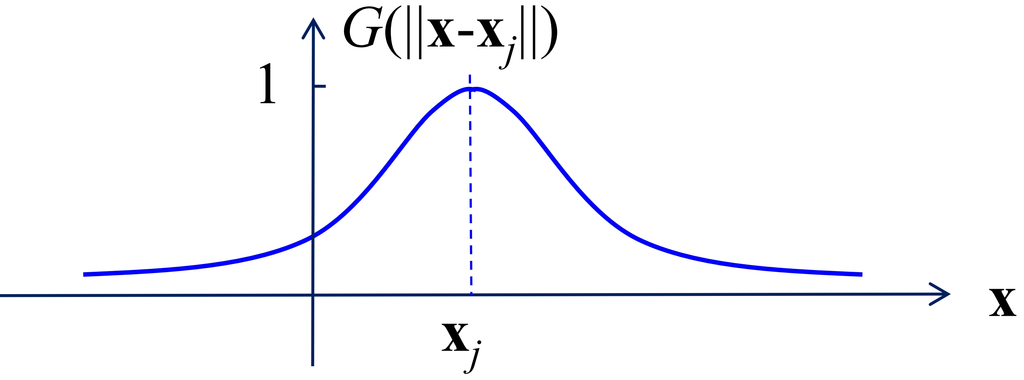
\includegraphics[width=0.85\linewidth]{fig/lec710.jpg}
% \end{center}
% \end{itemize}
% \end{frame}

% % 11
% \begin{frame}[c]
% \frametitle{Radial basis functions (cont.)}
% \begin{itemize}
% \item Thus approximation by Gaussian RBF becomes
% \[
% F(\mathbf{x})=\sum_jw_jG(||\mathbf{x}-\mathbf{x}_j||)
% \]
% \item Gaussians are universal approximators
		% \begin{itemize}
		% \item I.e., they form a complete basis
		% \end{itemize}
% \end{itemize}
% \begin{center}
% 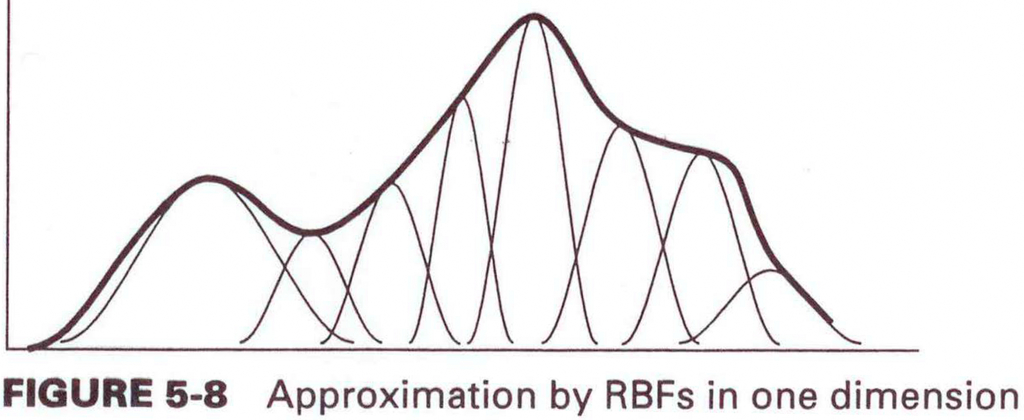
\includegraphics[width=0.99\linewidth]{fig/lec711.jpg}
% \end{center}
% \end{frame}

% % 12
% \begin{frame}[c]
% \frametitle{RBF net illustration}
% \begin{center}
% 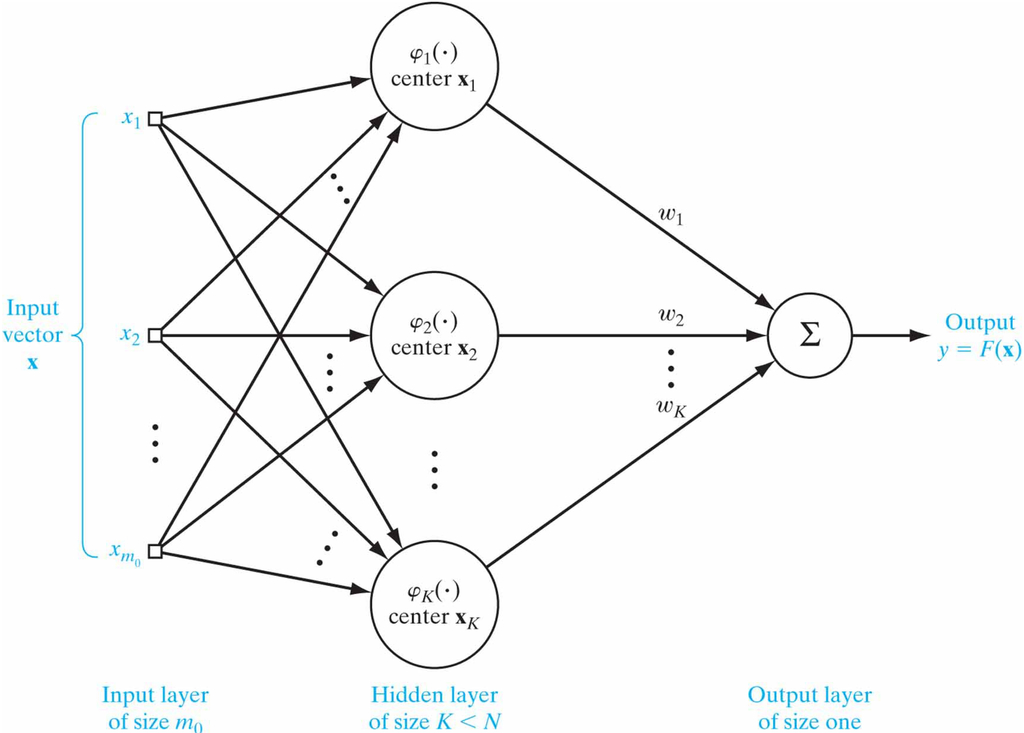
\includegraphics[width=0.99\linewidth]{fig/lec712.jpg}
% \end{center}
% \end{frame}

% % 13
% \begin{frame}[c]
% \frametitle{Remarks (cont.)}
% \begin{itemize}
% \item Other RBFs exist, but we won’t be using them
% \item Multiquadrics
% \[
% \varphi(x)=\sqrt{x^2+c^2}
% \]
% \item Inverse multiquadrics
% \[
% \varphi(x)=\frac{1}{\sqrt{x^2+c^2}}
% \]
% \item Micchelli's theorem (1986)
		% \begin{itemize}
		% \item Let $\{x_i\}$ be a set of 𝑁𝑁 distinct points, $\varphi(\cdot)$ be an RBF
		% \item Then the matrix $\phi_{ij}=\varphi(||\mathbf{x}_i-\mathbf{x}_j||)$ is non-singular
		% \end{itemize}
% \end{itemize}
% \end{frame}

% % 14
% \begin{frame}[c]
% \frametitle{Four questions to answer for RBF nets}
% \begin{itemize}
% \item If we want to use Gaussian RBFs to approximate a function specified by training data
		% \begin{enumerate}
		% \item How do we choose the Gaussian centers?
		% \item How do we determine the Gaussian widths?
		% \item How do we determine the weights $w_j$?
		% \item How do we select the number of bases?
		% \end{enumerate}
% \end{itemize}
% \end{frame}


% % 15
% \begin{frame}[c]
% \frametitle{1. How do we choose the Gaussian centers?}
% \begin{itemize}
% \item Easy way: select K data points at random
% \item Potentially better way: unsupervised clustering, e.g. using the K-means algorithm
% \end{itemize}
% \end{frame}

% % 16
% \begin{frame}[c]
% \frametitle{K-means algorithm}
% \begin{itemize}
% \item 𝛿Goal: Divide $N$ input patterns into $K$ clusters with minimum total variance In other words, partition patterns into $K$ clusters 𝐶𝐶
% \item In other words, partition patterns into $K$ clusters $C_j$ to minimize the following cost function
% \[
% J=\sum_{j=1}^K\sum_{i\in C_j} ||\mathbf{x}_i-\mathbf{u}_j||^2
% \]
% where $\mathbf{u}_j=\dfrac{1}{||C_j||}\sum_{i\in C_j}\mathbf{x}_i$ is  the mean (center) of cluster $j$
% \end{itemize}
% \end{frame}

% % 17
% \begin{frame}[c]
% \frametitle{K-means algorithm}
		% \begin{enumerate}
		% \item Choose a set of $K$ cluster centers randomly from the input patterns
		% \item Assign the $N$ input patterns to the $K$ clusters using the squared Euclidean distance rule:

% $x$ is assigned to $C_j$ if $||\mathbf{x}-\mathbf{u}_j||^2\le ||\mathbf{x}-\mathbf{u}_j||^2$ for all $i\neq j$
% \item Update cluster centers
% \[
% \mathbf{u}_j=\frac{1}{|C_j|}\sum_{i\in C_j}\mathbf{x}_i
% \]
% \item If any cluster center changes, go to step 2; else stop
% \end{enumerate}
% \end{frame}



% % 18
% \begin{frame}[c]
% \frametitle{K-means illustration}
% \begin{center}
% 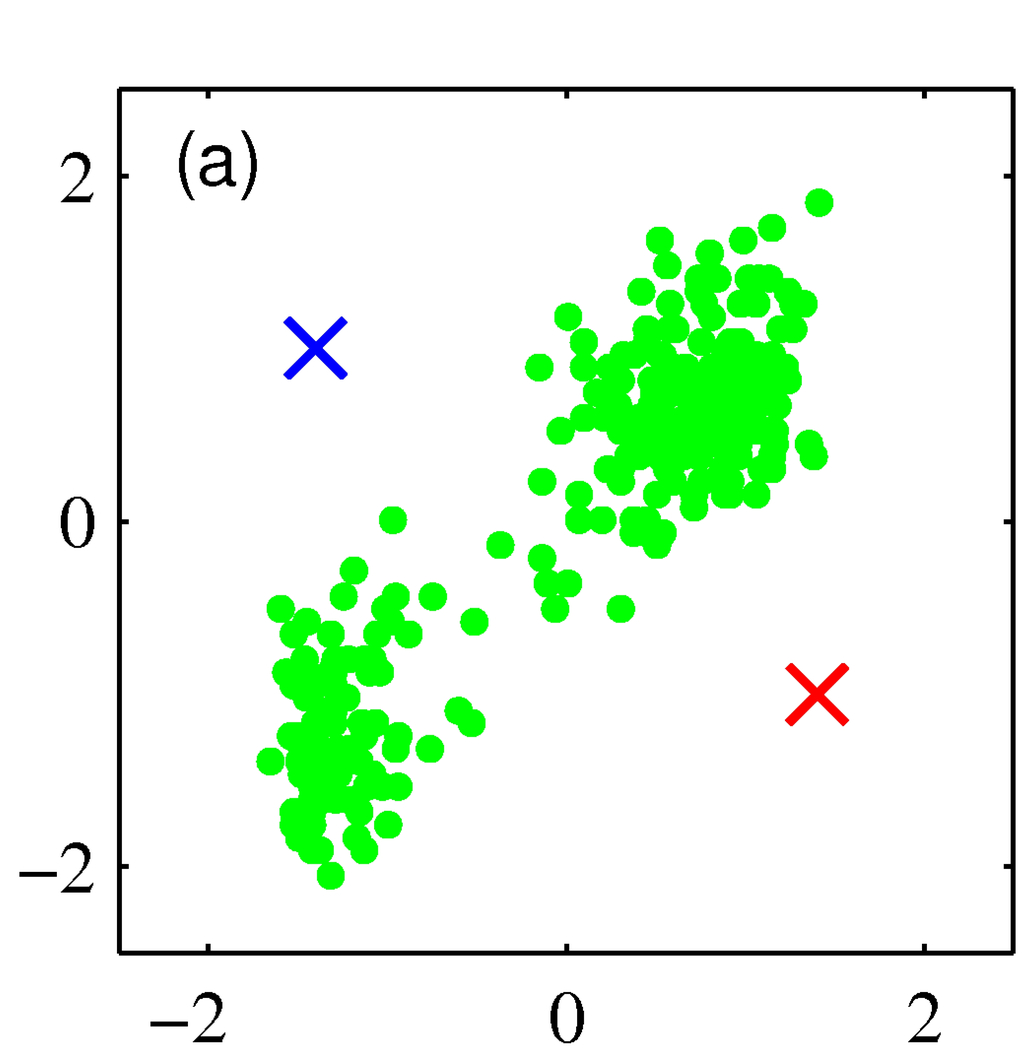
\includegraphics[width=0.65\textwidth]{fig/lec718.jpg}
% \end{center}
% \end{frame}


% % 19
% \begin{frame}[c]
% \frametitle{K-means illustration}
% \begin{center}
% 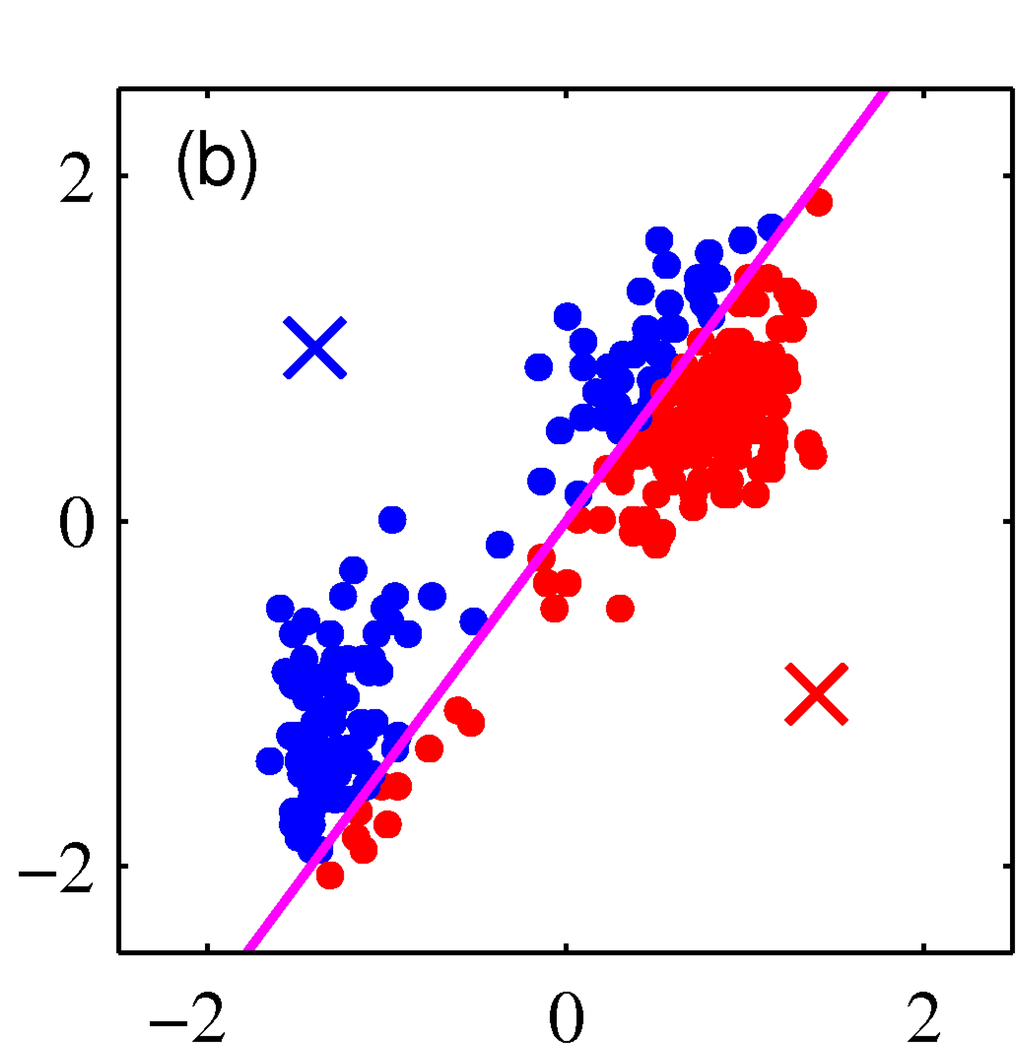
\includegraphics[width=0.65\textwidth]{fig/lec719.jpg}
% \end{center}
% \end{frame}
% % 20
% \begin{frame}[c]
% \frametitle{K-means illustration}
% \begin{center}
% 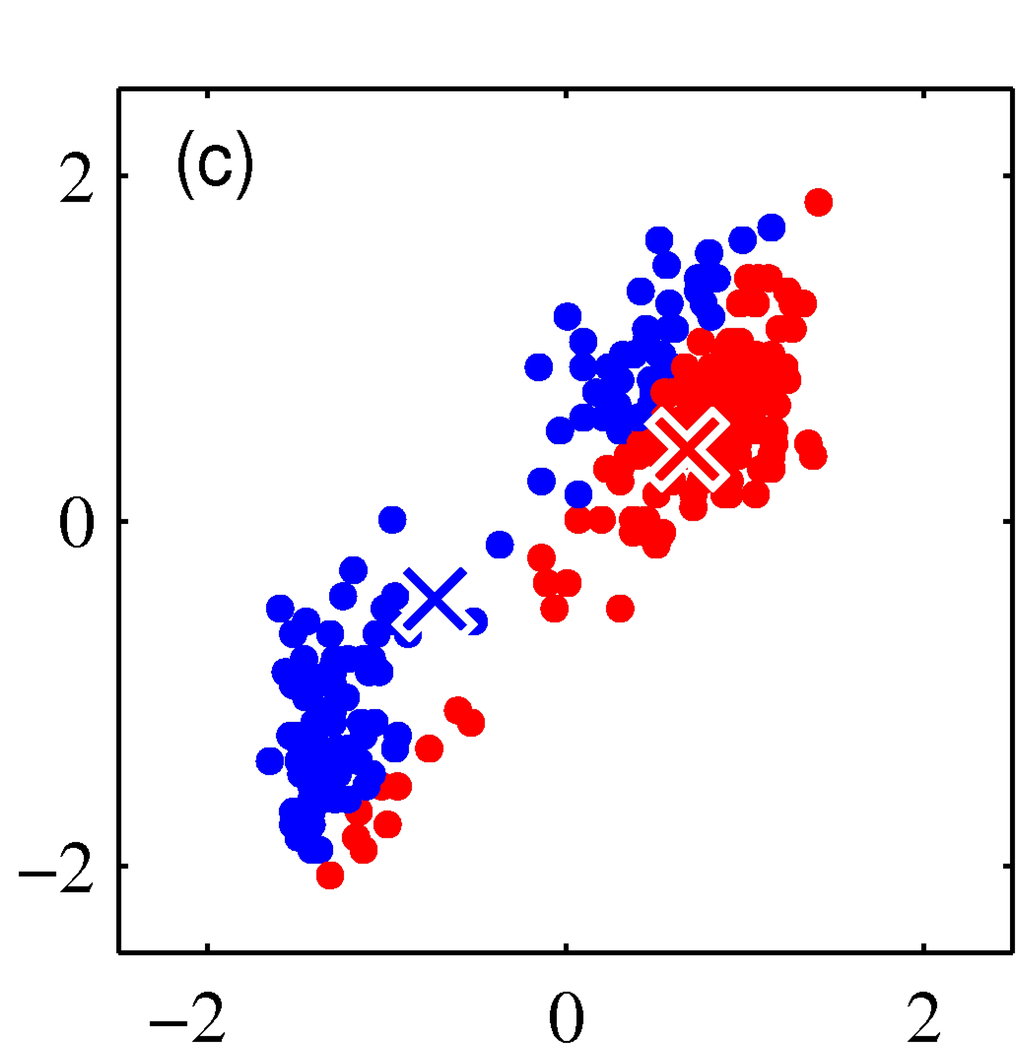
\includegraphics[width=0.65\textwidth]{fig/lec720.jpg}
% \end{center}
% \end{frame}
% % 21
% \begin{frame}[c]
% \frametitle{K-means illustration}
% \begin{center}
% 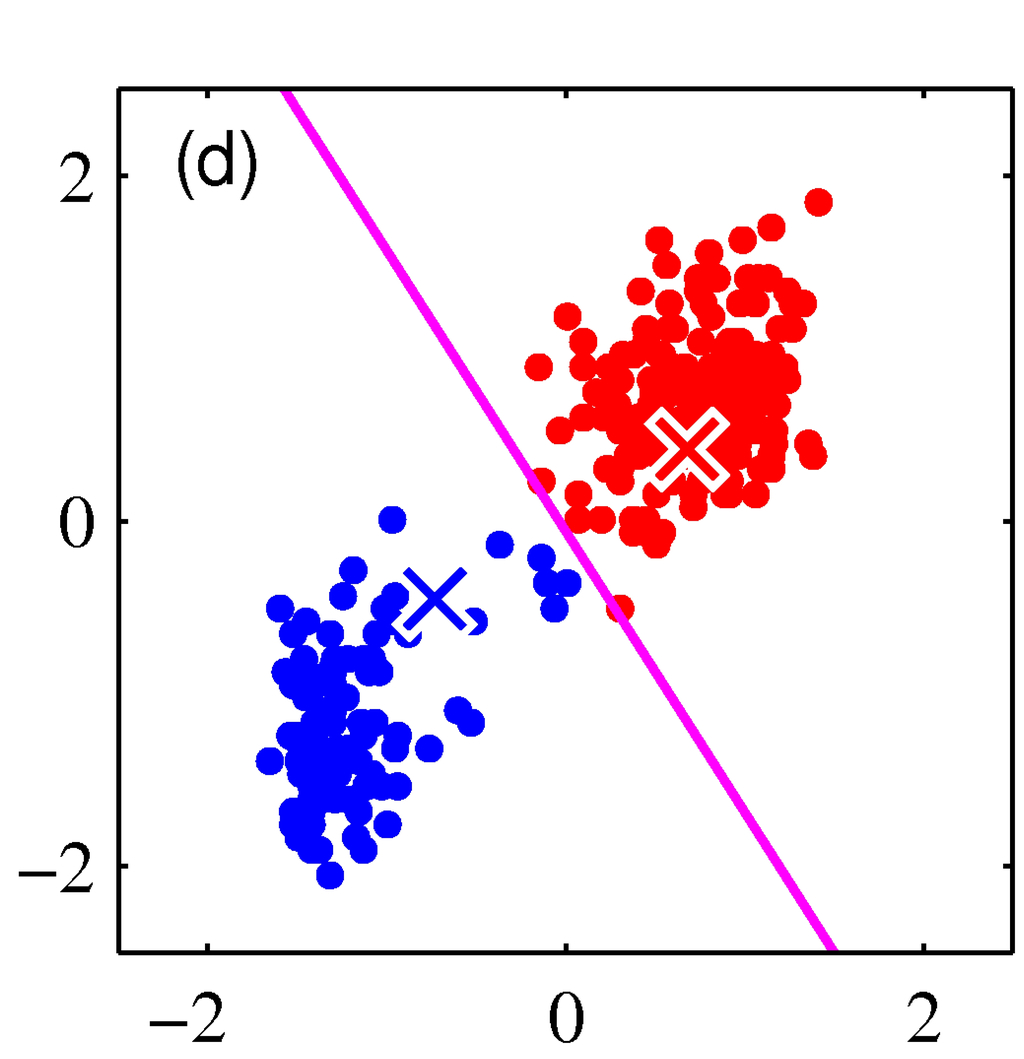
\includegraphics[width=0.65\textwidth]{fig/lec721.jpg}
% \end{center}
% \end{frame}

% % 22
% \begin{frame}[c]
% \frametitle{K-means illustration}
% \begin{center}
% 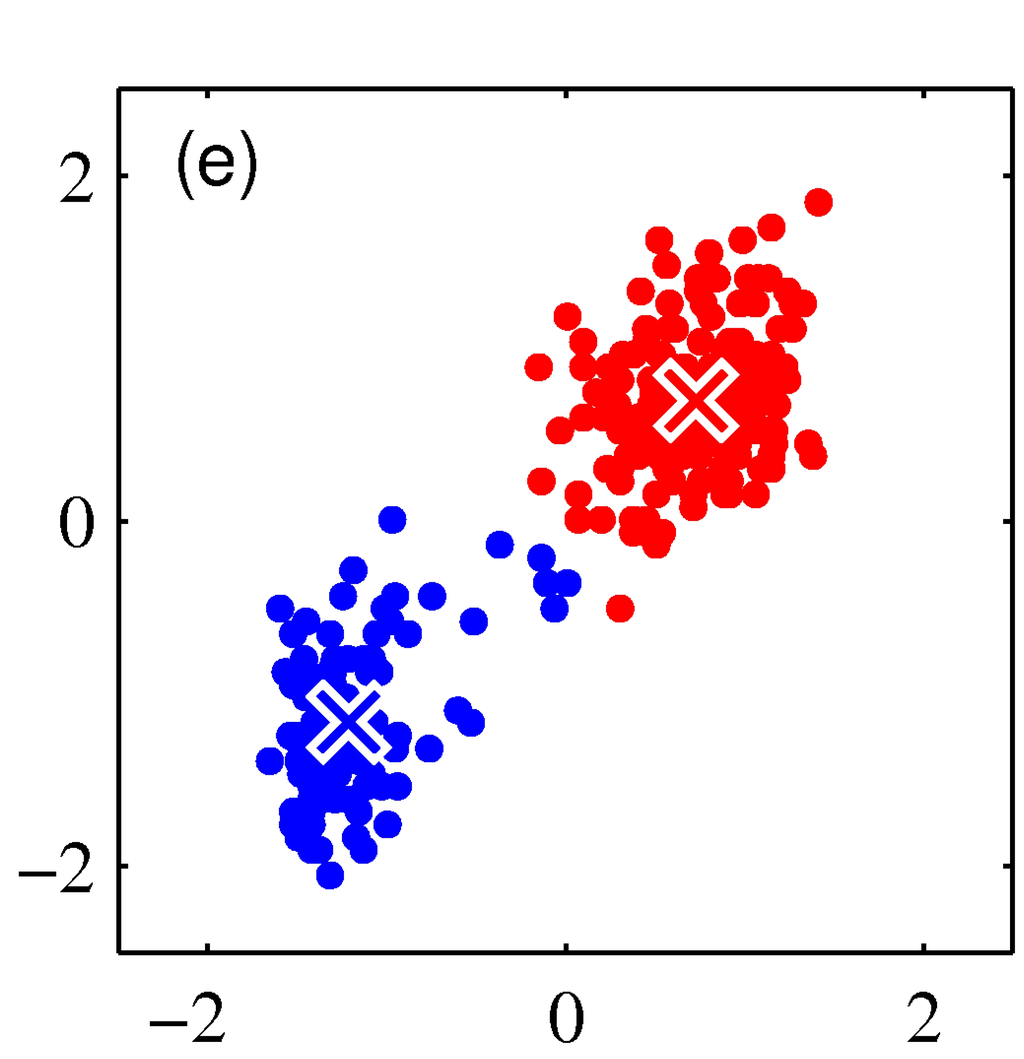
\includegraphics[width=0.65\textwidth]{fig/lec722.jpg}
% \end{center}
% \end{frame}

% % 23
% \begin{frame}[c]
% \frametitle{K-means illustration}
% \begin{center}
% 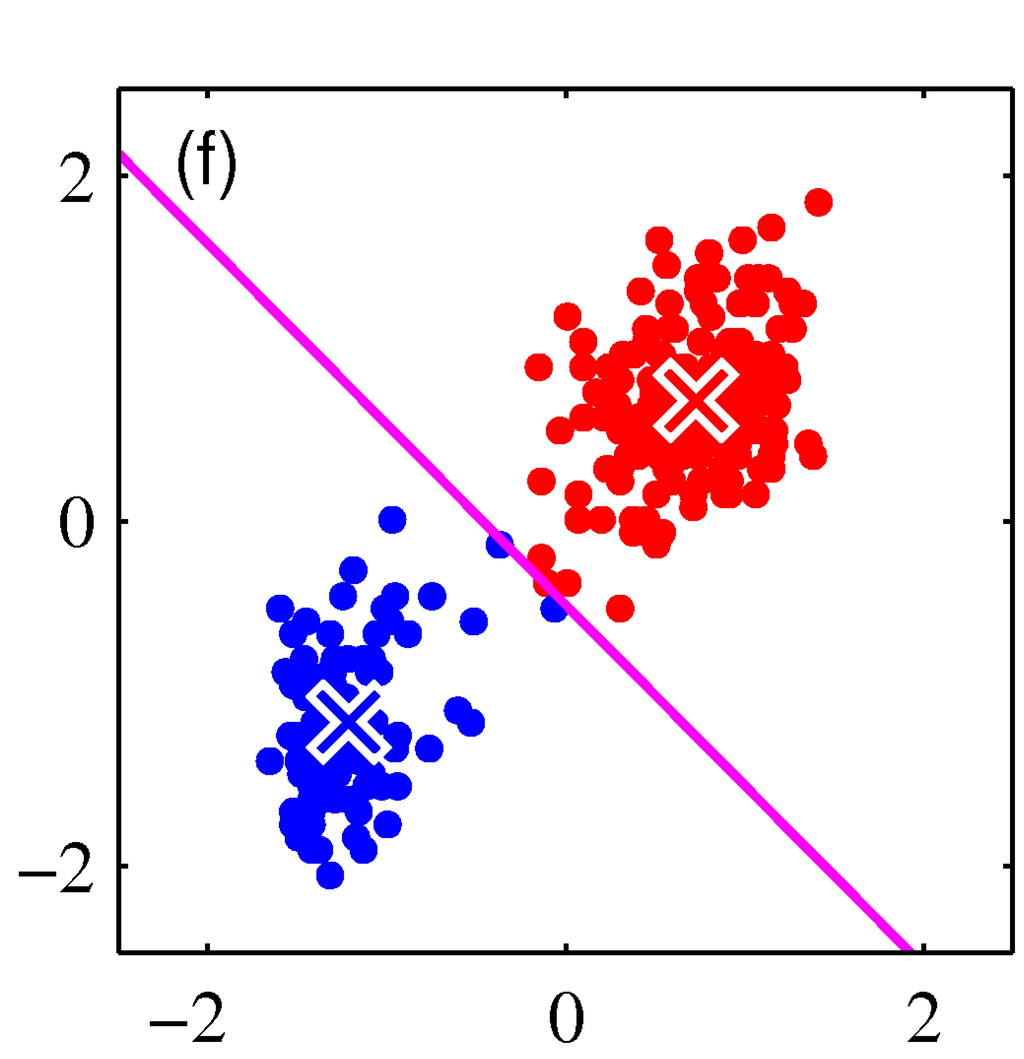
\includegraphics[width=0.65\textwidth]{fig/lec723.jpg}
% \end{center}
% \end{frame}

% % 24
% \begin{frame}[c]
% \frametitle{K-means illustration}
% \begin{center}
% 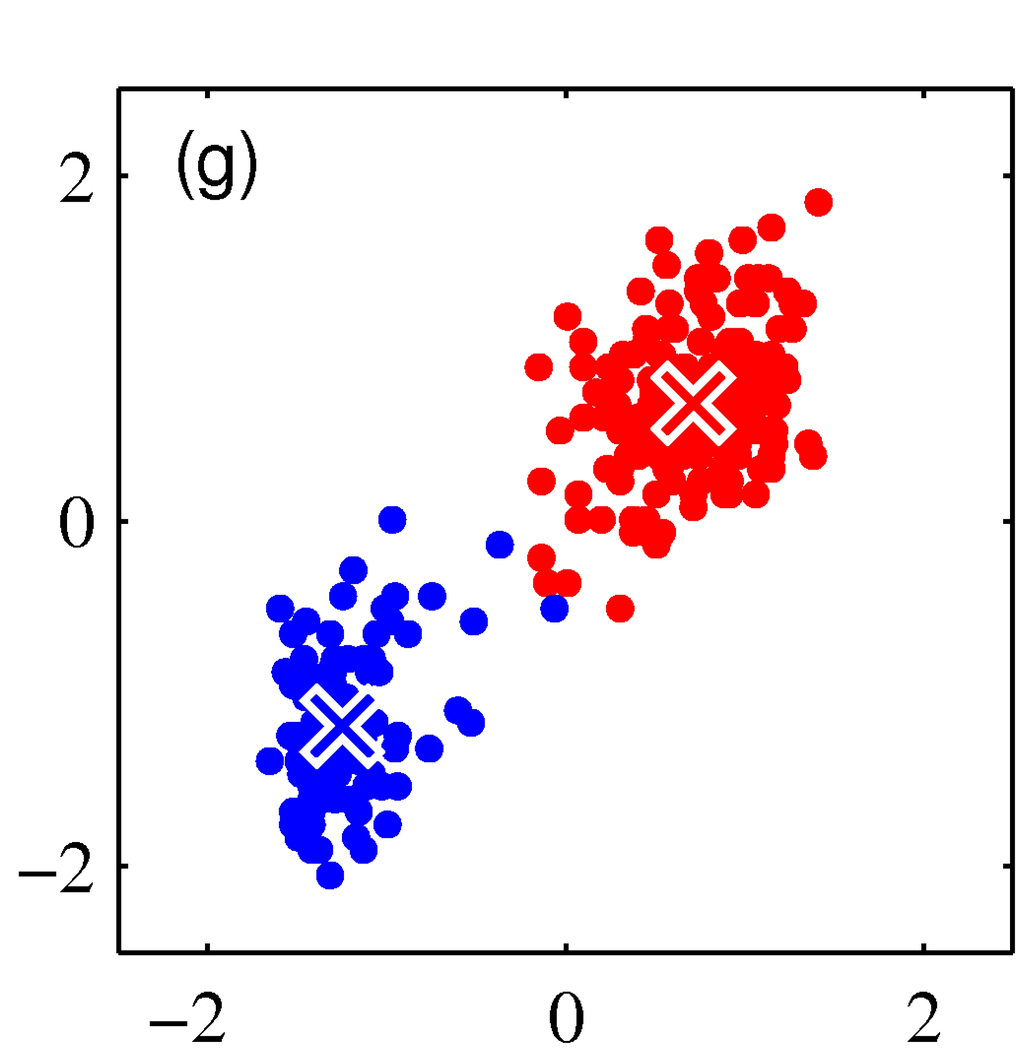
\includegraphics[width=0.65\textwidth]{fig/lec724.jpg}
% \end{center}
% \end{frame}

% % 25
% \begin{frame}[c]
% \frametitle{K-means illustration}
% \begin{center}
% 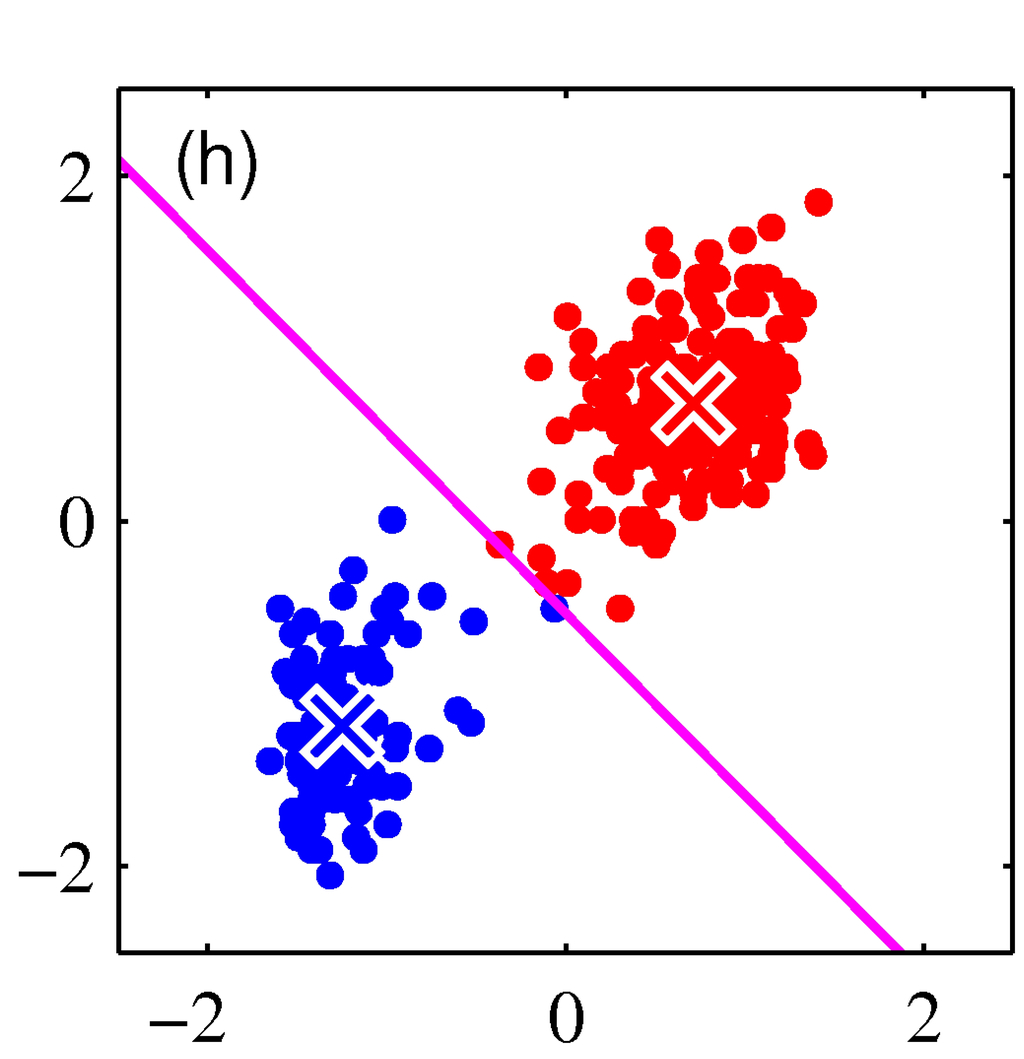
\includegraphics[width=0.65\textwidth]{fig/lec725.jpg}
% \end{center}
% \end{frame}
% % 26
% \begin{frame}[c]
% \frametitle{K-means illustration}
% \begin{center}
% 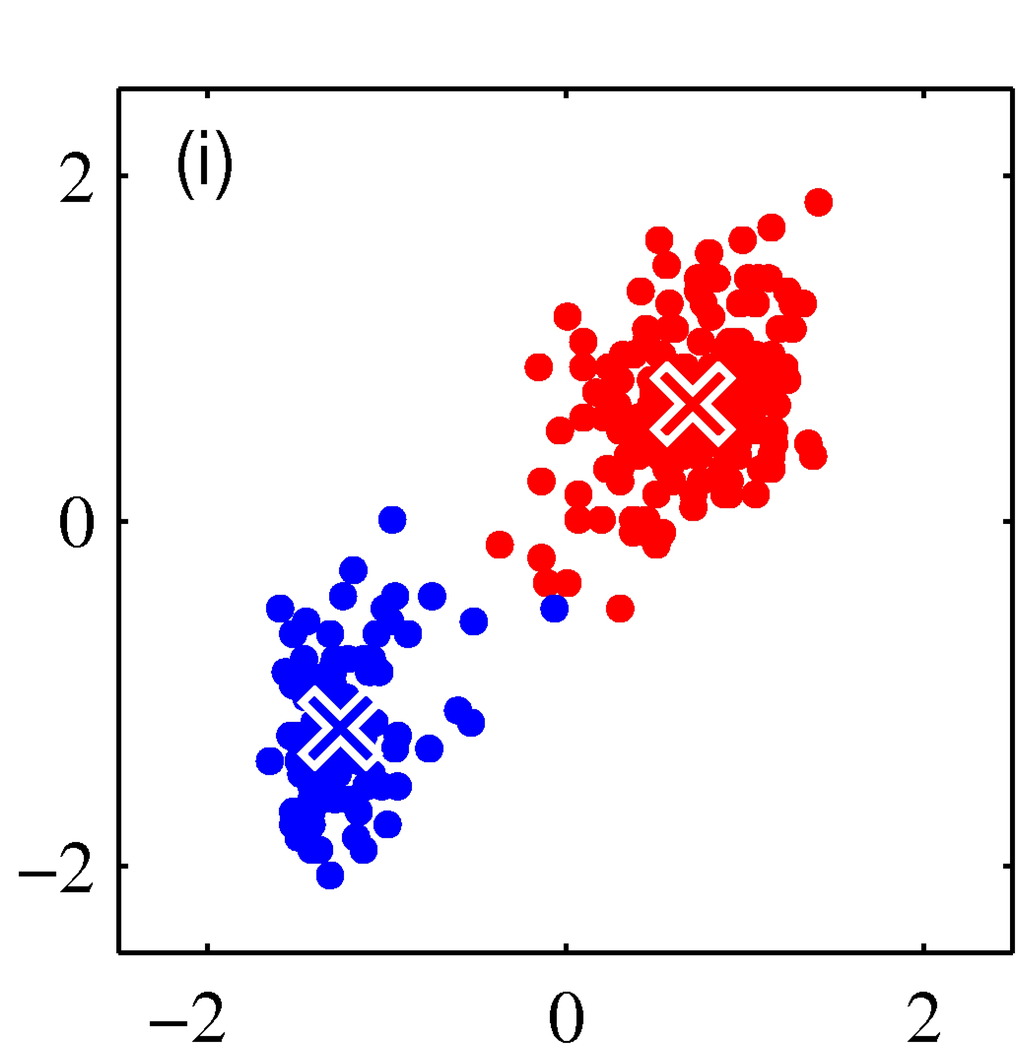
\includegraphics[width=0.65\textwidth]{fig/lec726.jpg}
% \end{center}
% \end{frame}
% % 27
% \begin{frame}[c]
% \frametitle{K-means cost function}
% \begin{center}
% 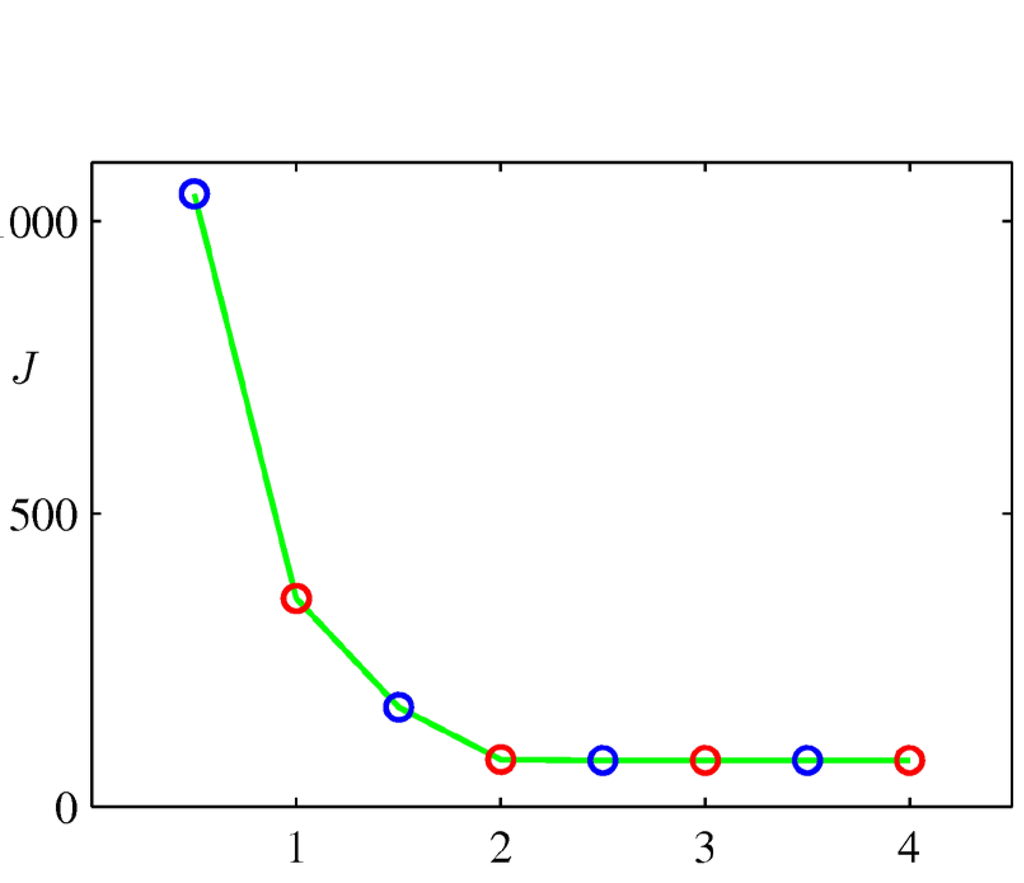
\includegraphics[width=0.65\textwidth]{fig/lec727.jpg}
% \end{center}
% \end{frame}

% % 28
% \begin{frame}[c]
% \frametitle{K-means algorithm remarks}
		% \begin{itemize}
		% \item The K-means algorithm always converges, but only to a local minimum
		% \end{itemize}
% \end{frame}


% % 29
% \begin{frame}[c]
% \frametitle{2. How to determine the Gaussian widths?}
		% \begin{itemize}
		% \item Once cluster centers are determined, the variance within each cluster can be set to
		% \[
		% \sigma_j^2=\frac{1}{C_j}\sum_{i\in C_j}||\mathbf{u}_j-\mathbf{x}_i||^2
		% \]
		% \begin{itemize}
		% \item {\bf Remark:} to simplify the RBF net design, all clusters can assume the same Gaussian width:
% \[
% \sigma=\frac{d_{\max}}{\sqrt{2K}}
% \]
% where $d_{\max}$ is the maximum distance between the $K$ cluster centers
		% \end{itemize}
		% \end{itemize}
% \end{frame}

% % 30
% \begin{frame}[c]
% \frametitle{3. How do we determine the weights $w_j$?}
		% \begin{itemize}
		% \item With the hidden layer decided, weight training can be treated as a linear regression problem 
		% \[
		% \Phi_\mathbf{w}=\mathbf{d}
		% \]
		% \item Can solve using the LMS algorithm
		% \item The textbook discusses recursive least squares (RLS) solutions
		% \item Can also solve in one shot using the pseudo-inverse
		% \[
		% \mathbf{w}=\Phi^+\mathbf{d}=(\Phi^T\Phi)^{-1}\Phi^T\mathbf{d}
		% \]
		% \item Note that a bias term needs to be included in ${\Phi}$
		% \end{itemize}
% \end{frame}



% % 31
% \begin{frame}[c]
% \frametitle{4. How do we select the number of bases?}
		% \begin{itemize}
		% \item The same problem as that of selecting the size of an MLP for classification
		% \item The short answer: (cross-)validation
		% \item The long answer: by balancing bias and variance
		% \end{itemize}
% \end{frame}



% % 32
% \begin{frame}[c]
% \frametitle{Bias and variance}
		% \begin{itemize}
		% \item Bias: training error
		% \begin{itemize}
		% \item Difference between desired output and actual output for a particular training sample
		% \end{itemize}
		% \item Variance: generalization error
		% \begin{itemize}
		% \item  difference between the learned function from a particular training sample and the function derived from all training samples
		% \end{itemize}
		% \item Two extreme cases: zero bias and zero variance
		% \item A good-sized model is one where both bias and variance are low
		% \end{itemize}
% \end{frame}


% % 33
% \begin{frame}[c]
% \frametitle{RBF net training summary}
		% \begin{itemize}
		% \item To train
		% \begin{enumerate}
		% \item Choose the Gaussian centers using K-means, etc.
		% \item Determine the Gaussian widths as the variance of each cluster, or using $d_{\max}$ 
		% \item Determine the weights $w_j$ using linear regression
		% \end{enumerate}
		% \item Select the number of bases using (cross-)validation
		% \end{itemize}
% \end{frame}


% % 34
% \begin{frame}[c]
% \frametitle{RBF net illustration}
% \begin{center}
% 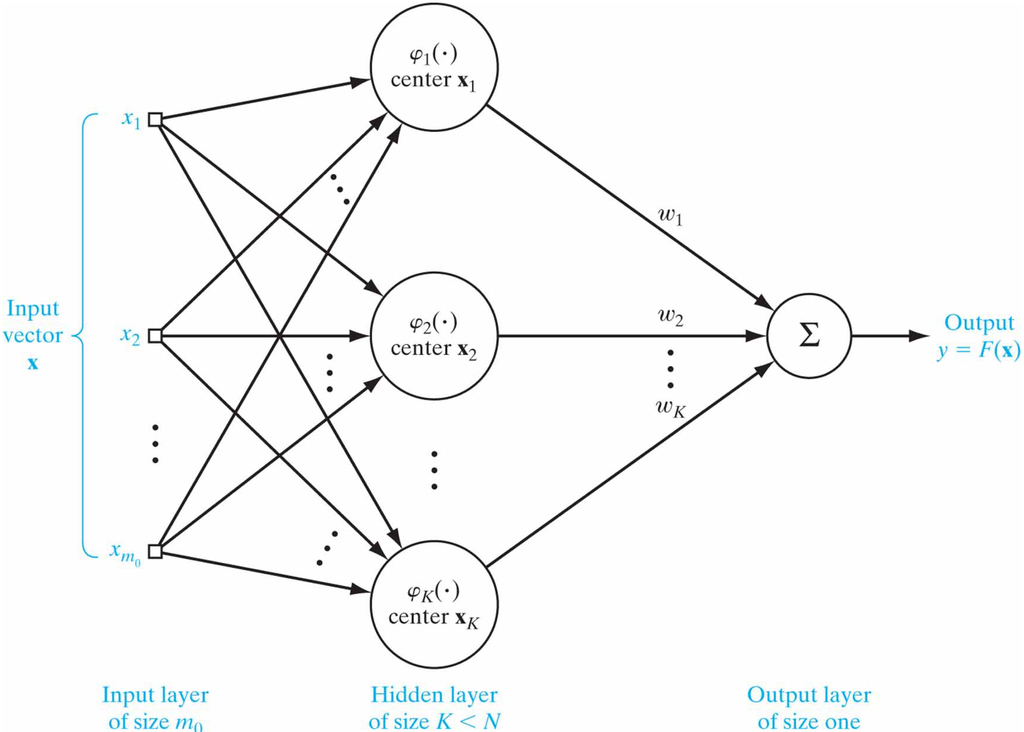
\includegraphics[width=0.99\linewidth]{fig/lec734.jpg}
% \end{center}
% \end{frame}



% % 35
% \begin{frame}[c]
% \frametitle{Comparison between RBF net and MLP}
		% \begin{itemize}
		% \item For RBF nets, bases are local, while for MLP, ``bases'' are global
		% \item Generally, more bases are needed for an RBF net than hidden units for an MLP
		% \item Training is more efficient for RBF nets
		% \end{itemize}
% \end{frame}

% % 36
% \begin{frame}[t]
% \frametitle{XOR problem, again}
% \begin{columns}
% \column{.5\textwidth}

		% \begin{itemize}
		% \item RBF nets can also be applied to pattern classification problems
		% \begin{itemize}
		% \item XOR problem revisited
		% \end{itemize}
		% \end{itemize}
% \column{.5\textwidth}
% \begin{center}
% 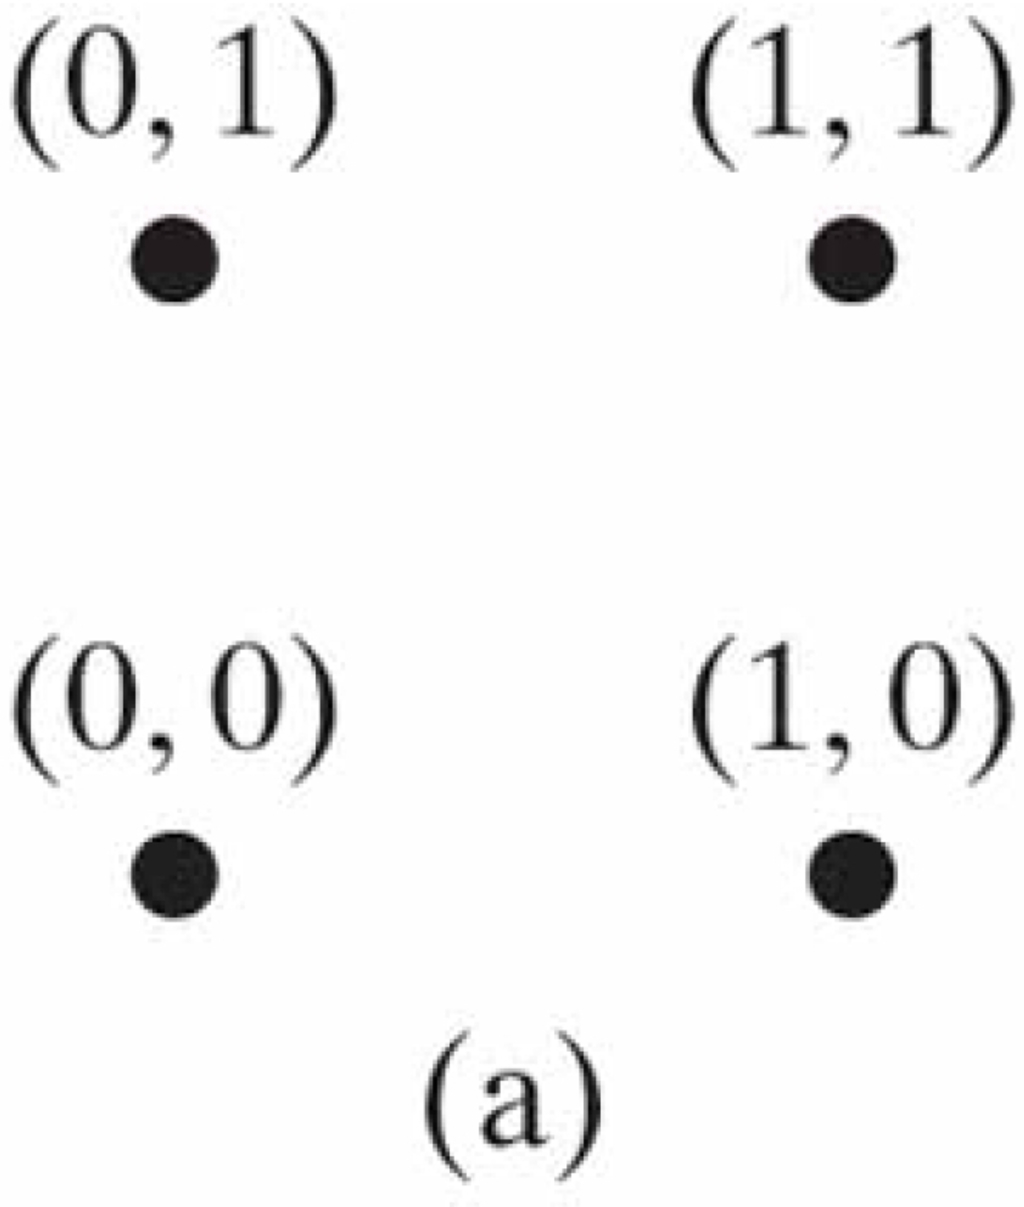
\includegraphics[width=0.3\linewidth]{fig/lec736.jpg}
% \end{center}
% Let 

% $\phi_1(x)=\exp (-||x-t_1||)^2$

% $\phi_2(x)=\exp (-||x-t_2||)^2$

% where
% \[\begin{array}{c}
% t_1=[1,1]^T\\
% t_2=[0,0]^T
% \end{array}\]
% \end{columns}
% \end{frame}


% % 37
% \begin{frame}[c]
% \frametitle{XOR problem (cont.)}
% \begin{center}
% 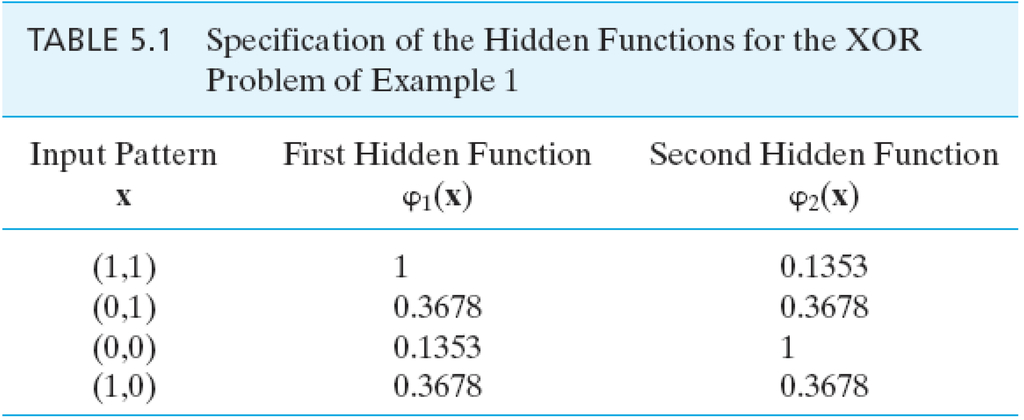
\includegraphics[width=0.95\linewidth]{fig/lec737.jpg}
% \end{center}
% \end{frame}


% % 38
% \begin{frame}
% \frametitle{XOR problem, again}
% \begin{columns}
% \column{.5\textwidth}
		% \begin{itemize}
		% \item RBF nets can also be applied to pattern classification problems
		% \begin{itemize}
		% \item XOR problem revisited
		% \end{itemize}
		% \end{itemize}
% \column{.5\textwidth}
% \begin{center}\hspace*{-5mm}
% 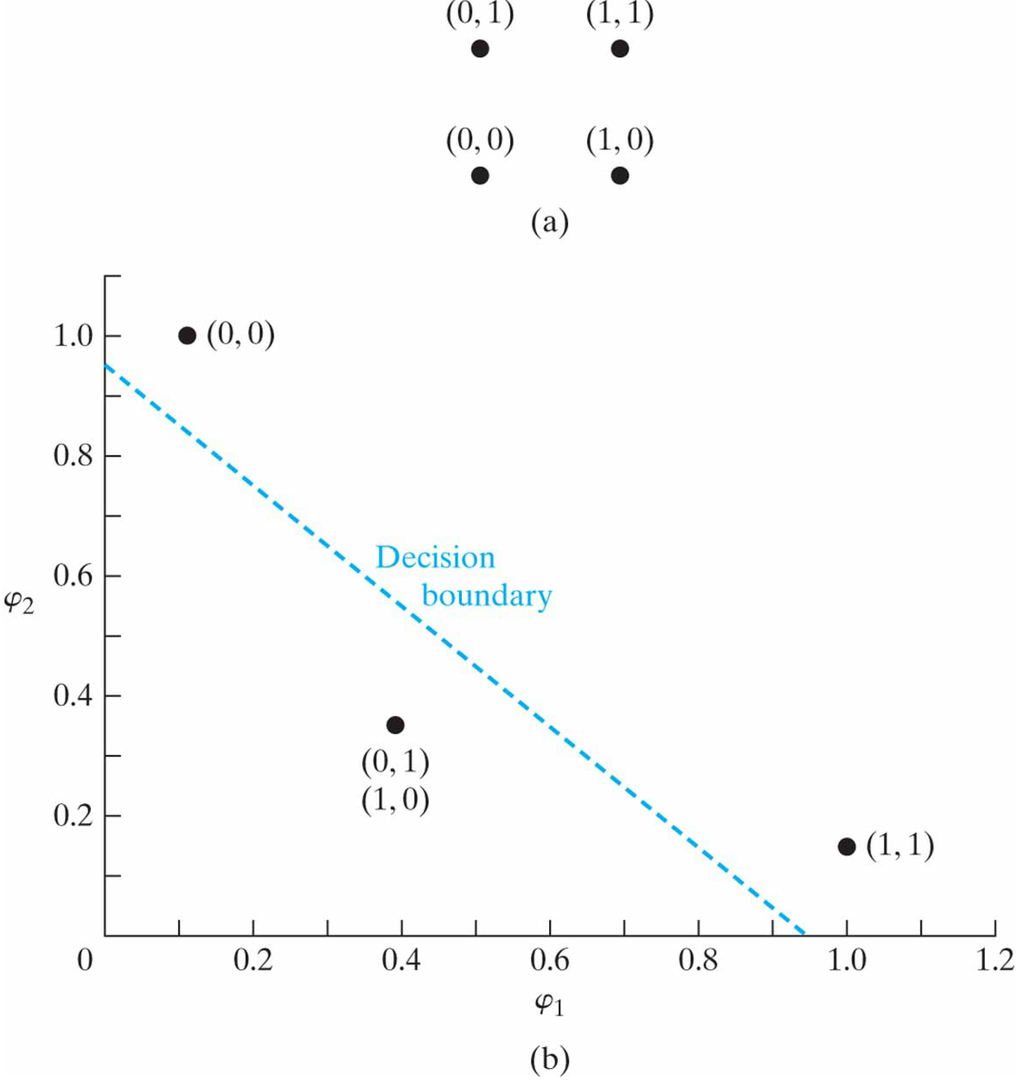
\includegraphics[width=1.15\linewidth]{fig/lec738.jpg}
% \end{center}
% \end{columns}
% \end{frame}


% % 39
% \begin{frame}
% \frametitle{RBF net on double moon data, $d=-5$}
% \begin{center}
% 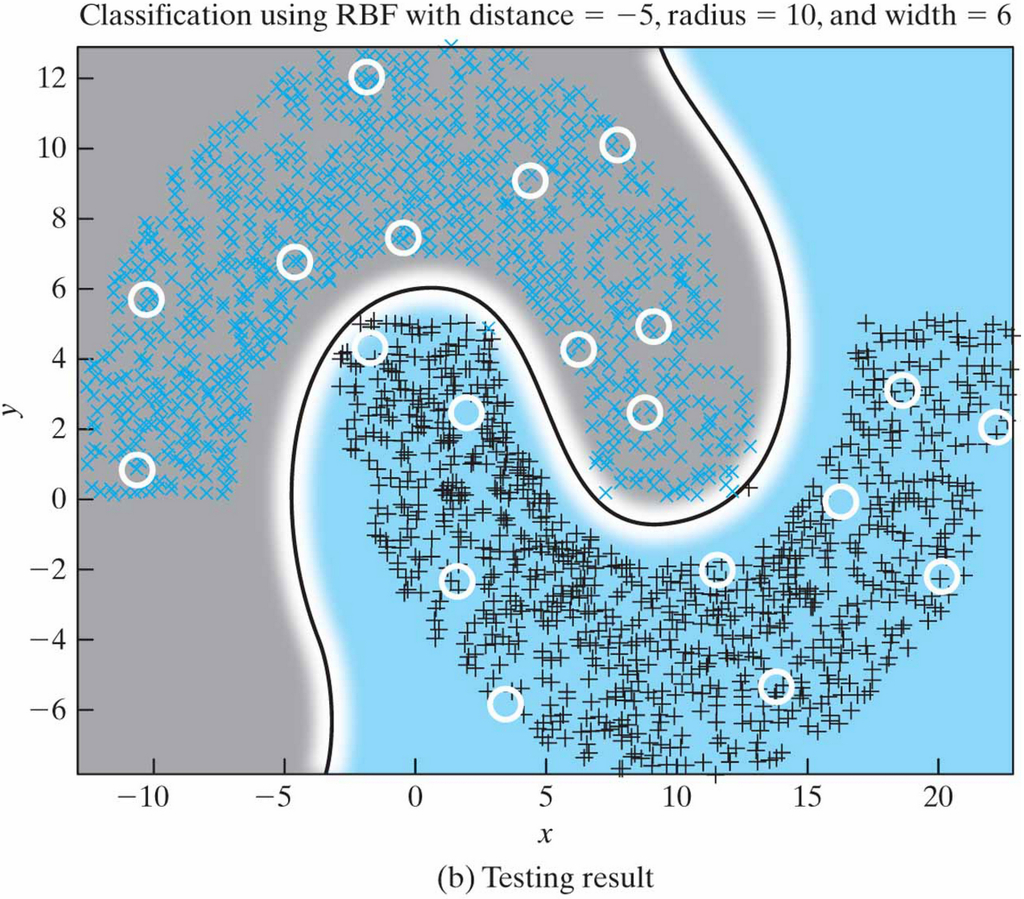
\includegraphics[width=0.8\linewidth]{fig/lec739.jpg}
% \end{center}
% \end{frame}


% % 40
% \begin{frame}
% \frametitle{RBF net on double moon data, $d=-5$}
% \begin{center}
% 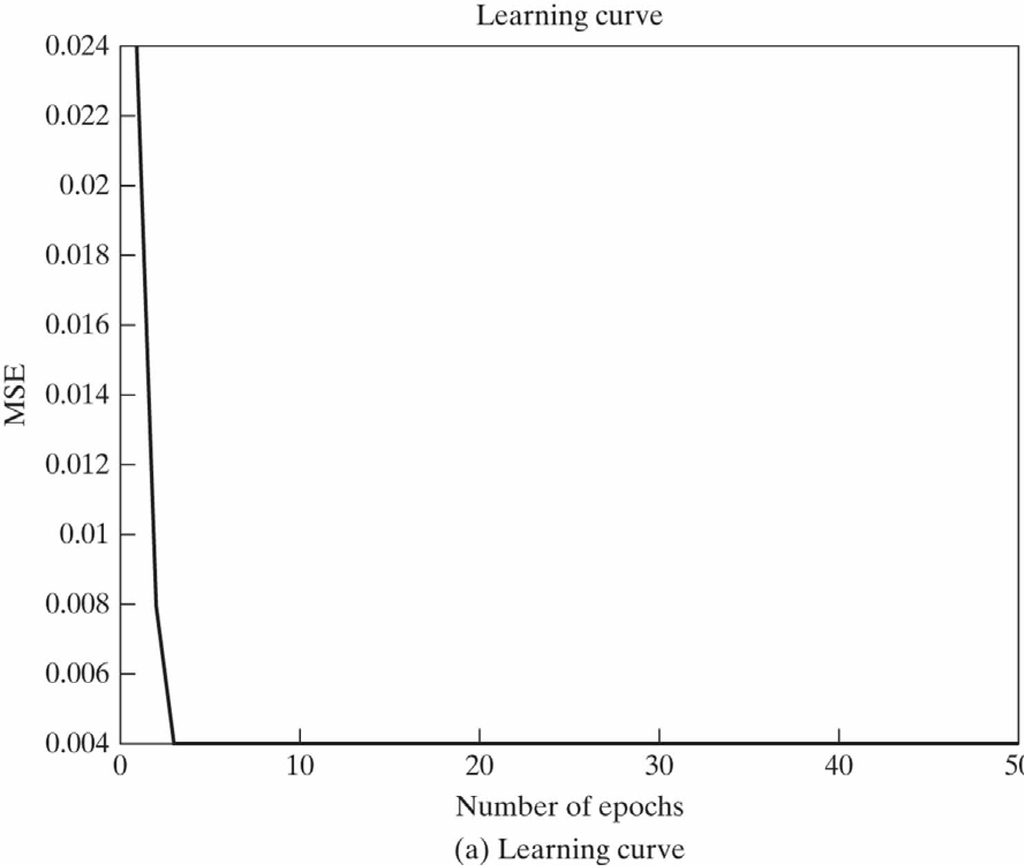
\includegraphics[width=0.8\linewidth]{fig/lec740.jpg}
% \end{center}
% \end{frame}

% % 41
% \begin{frame}
% \frametitle{RBF net on double moon data, $d=-6$}
% \begin{center}
% 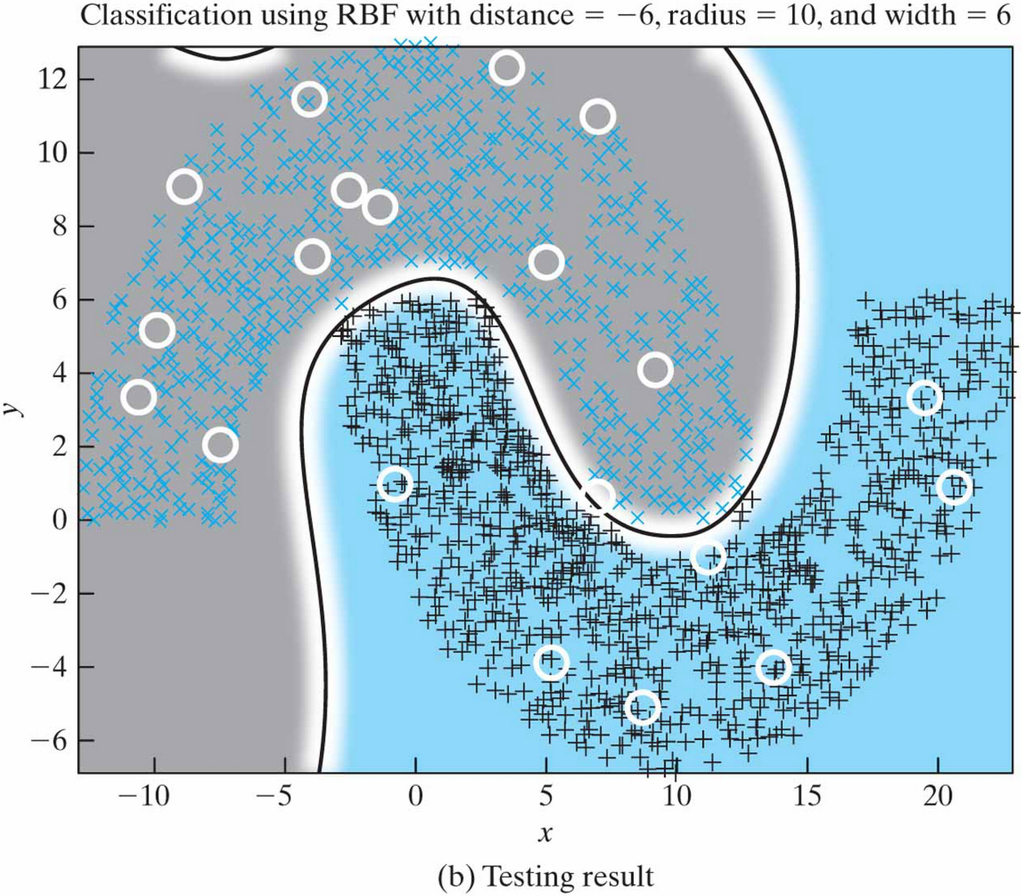
\includegraphics[width=0.8\linewidth]{fig/lec741.jpg}
% \end{center}
% \end{frame}

% % 42
% \begin{frame}
% \frametitle{RBF net on double moon data, $d=-6$}
% \begin{center}
% 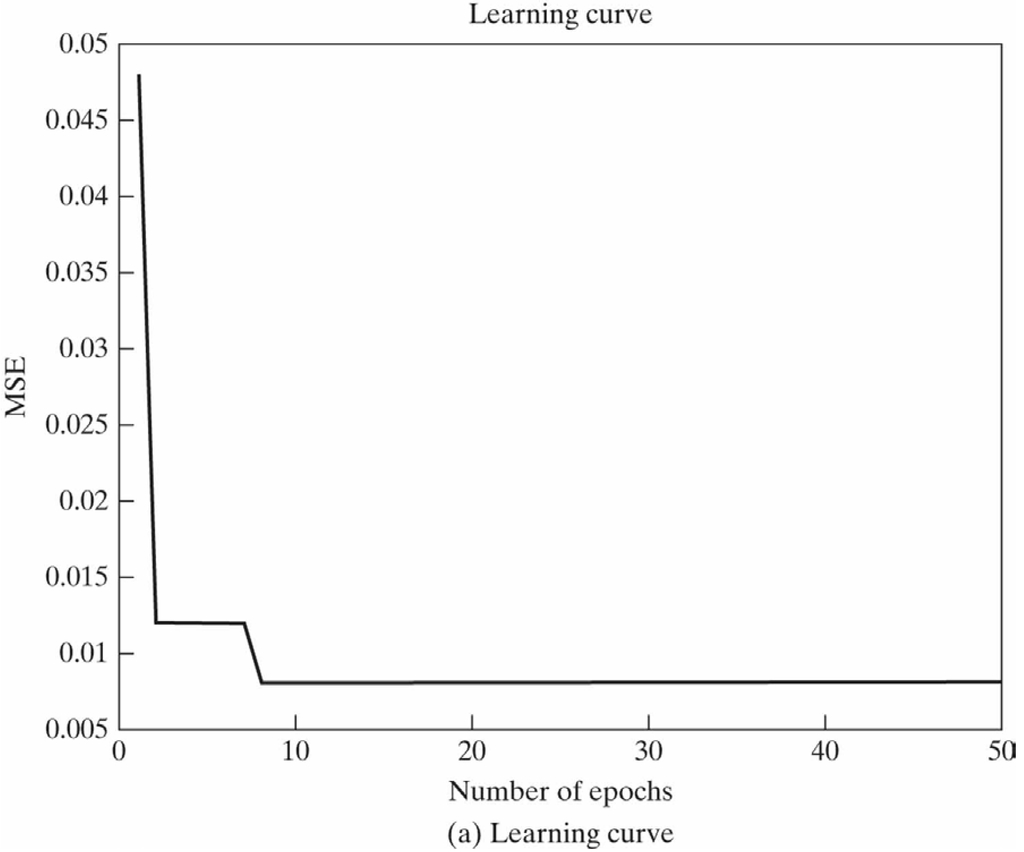
\includegraphics[width=0.8\linewidth]{fig/lec742.jpg}
% \end{center}
% \end{frame}






\begin{frame}
\begin{center}
\chuhao Thank you! %\fontspec{LHANDW.TTF}
\end{center}
\end{frame}
\end{document}
